% Options for packages loaded elsewhere
\PassOptionsToPackage{unicode}{hyperref}
\PassOptionsToPackage{hyphens}{url}
%
\documentclass[
]{book}
\usepackage{lmodern}
\usepackage{amssymb,amsmath}
\usepackage{ifxetex,ifluatex}
\ifnum 0\ifxetex 1\fi\ifluatex 1\fi=0 % if pdftex
  \usepackage[T1]{fontenc}
  \usepackage[utf8]{inputenc}
  \usepackage{textcomp} % provide euro and other symbols
\else % if luatex or xetex
  \usepackage{unicode-math}
  \defaultfontfeatures{Scale=MatchLowercase}
  \defaultfontfeatures[\rmfamily]{Ligatures=TeX,Scale=1}
\fi
% Use upquote if available, for straight quotes in verbatim environments
\IfFileExists{upquote.sty}{\usepackage{upquote}}{}
\IfFileExists{microtype.sty}{% use microtype if available
  \usepackage[]{microtype}
  \UseMicrotypeSet[protrusion]{basicmath} % disable protrusion for tt fonts
}{}
\makeatletter
\@ifundefined{KOMAClassName}{% if non-KOMA class
  \IfFileExists{parskip.sty}{%
    \usepackage{parskip}
  }{% else
    \setlength{\parindent}{0pt}
    \setlength{\parskip}{6pt plus 2pt minus 1pt}}
}{% if KOMA class
  \KOMAoptions{parskip=half}}
\makeatother
\usepackage{xcolor}
\IfFileExists{xurl.sty}{\usepackage{xurl}}{} % add URL line breaks if available
\IfFileExists{bookmark.sty}{\usepackage{bookmark}}{\usepackage{hyperref}}
\hypersetup{
  pdftitle={Introduction to Theoretical Ecology},
  pdfauthor={Instructor: Po-Ju Ke \textasciitilde\textasciitilde\textasciitilde\textasciitilde\textasciitilde{} Teaching Assistant: Ching-Lin Huang (Andy)},
  hidelinks,
  pdfcreator={LaTeX via pandoc}}
\urlstyle{same} % disable monospaced font for URLs
\usepackage{color}
\usepackage{fancyvrb}
\newcommand{\VerbBar}{|}
\newcommand{\VERB}{\Verb[commandchars=\\\{\}]}
\DefineVerbatimEnvironment{Highlighting}{Verbatim}{commandchars=\\\{\}}
% Add ',fontsize=\small' for more characters per line
\usepackage{framed}
\definecolor{shadecolor}{RGB}{248,248,248}
\newenvironment{Shaded}{\begin{snugshade}}{\end{snugshade}}
\newcommand{\AlertTok}[1]{\textcolor[rgb]{0.94,0.16,0.16}{#1}}
\newcommand{\AnnotationTok}[1]{\textcolor[rgb]{0.56,0.35,0.01}{\textbf{\textit{#1}}}}
\newcommand{\AttributeTok}[1]{\textcolor[rgb]{0.77,0.63,0.00}{#1}}
\newcommand{\BaseNTok}[1]{\textcolor[rgb]{0.00,0.00,0.81}{#1}}
\newcommand{\BuiltInTok}[1]{#1}
\newcommand{\CharTok}[1]{\textcolor[rgb]{0.31,0.60,0.02}{#1}}
\newcommand{\CommentTok}[1]{\textcolor[rgb]{0.56,0.35,0.01}{\textit{#1}}}
\newcommand{\CommentVarTok}[1]{\textcolor[rgb]{0.56,0.35,0.01}{\textbf{\textit{#1}}}}
\newcommand{\ConstantTok}[1]{\textcolor[rgb]{0.00,0.00,0.00}{#1}}
\newcommand{\ControlFlowTok}[1]{\textcolor[rgb]{0.13,0.29,0.53}{\textbf{#1}}}
\newcommand{\DataTypeTok}[1]{\textcolor[rgb]{0.13,0.29,0.53}{#1}}
\newcommand{\DecValTok}[1]{\textcolor[rgb]{0.00,0.00,0.81}{#1}}
\newcommand{\DocumentationTok}[1]{\textcolor[rgb]{0.56,0.35,0.01}{\textbf{\textit{#1}}}}
\newcommand{\ErrorTok}[1]{\textcolor[rgb]{0.64,0.00,0.00}{\textbf{#1}}}
\newcommand{\ExtensionTok}[1]{#1}
\newcommand{\FloatTok}[1]{\textcolor[rgb]{0.00,0.00,0.81}{#1}}
\newcommand{\FunctionTok}[1]{\textcolor[rgb]{0.00,0.00,0.00}{#1}}
\newcommand{\ImportTok}[1]{#1}
\newcommand{\InformationTok}[1]{\textcolor[rgb]{0.56,0.35,0.01}{\textbf{\textit{#1}}}}
\newcommand{\KeywordTok}[1]{\textcolor[rgb]{0.13,0.29,0.53}{\textbf{#1}}}
\newcommand{\NormalTok}[1]{#1}
\newcommand{\OperatorTok}[1]{\textcolor[rgb]{0.81,0.36,0.00}{\textbf{#1}}}
\newcommand{\OtherTok}[1]{\textcolor[rgb]{0.56,0.35,0.01}{#1}}
\newcommand{\PreprocessorTok}[1]{\textcolor[rgb]{0.56,0.35,0.01}{\textit{#1}}}
\newcommand{\RegionMarkerTok}[1]{#1}
\newcommand{\SpecialCharTok}[1]{\textcolor[rgb]{0.00,0.00,0.00}{#1}}
\newcommand{\SpecialStringTok}[1]{\textcolor[rgb]{0.31,0.60,0.02}{#1}}
\newcommand{\StringTok}[1]{\textcolor[rgb]{0.31,0.60,0.02}{#1}}
\newcommand{\VariableTok}[1]{\textcolor[rgb]{0.00,0.00,0.00}{#1}}
\newcommand{\VerbatimStringTok}[1]{\textcolor[rgb]{0.31,0.60,0.02}{#1}}
\newcommand{\WarningTok}[1]{\textcolor[rgb]{0.56,0.35,0.01}{\textbf{\textit{#1}}}}
\usepackage{longtable,booktabs}
% Correct order of tables after \paragraph or \subparagraph
\usepackage{etoolbox}
\makeatletter
\patchcmd\longtable{\par}{\if@noskipsec\mbox{}\fi\par}{}{}
\makeatother
% Allow footnotes in longtable head/foot
\IfFileExists{footnotehyper.sty}{\usepackage{footnotehyper}}{\usepackage{footnote}}
\makesavenoteenv{longtable}
\usepackage{graphicx,grffile}
\makeatletter
\def\maxwidth{\ifdim\Gin@nat@width>\linewidth\linewidth\else\Gin@nat@width\fi}
\def\maxheight{\ifdim\Gin@nat@height>\textheight\textheight\else\Gin@nat@height\fi}
\makeatother
% Scale images if necessary, so that they will not overflow the page
% margins by default, and it is still possible to overwrite the defaults
% using explicit options in \includegraphics[width, height, ...]{}
\setkeys{Gin}{width=\maxwidth,height=\maxheight,keepaspectratio}
% Set default figure placement to htbp
\makeatletter
\def\fps@figure{htbp}
\makeatother
\setlength{\emergencystretch}{3em} % prevent overfull lines
\providecommand{\tightlist}{%
  \setlength{\itemsep}{0pt}\setlength{\parskip}{0pt}}
\setcounter{secnumdepth}{5}
\usepackage{booktabs}
\usepackage{amsthm}
\makeatletter
\def\thm@space@setup{%
  \thm@preskip=8pt plus 2pt minus 4pt
  \thm@postskip=\thm@preskip
}
\makeatother
\usepackage{booktabs}
\usepackage{longtable}
\usepackage{array}
\usepackage{multirow}
\usepackage{wrapfig}
\usepackage{float}
\usepackage{colortbl}
\usepackage{pdflscape}
\usepackage{tabu}
\usepackage{threeparttable}
\usepackage{threeparttablex}
\usepackage[normalem]{ulem}
\usepackage{makecell}
\usepackage{xcolor}
\usepackage[]{natbib}
\bibliographystyle{apalike}

\title{Introduction to Theoretical Ecology}
\author{Instructor: Po-Ju Ke \(~~~~~\) Teaching Assistant: Ching-Lin Huang (Andy)}
\date{2022 Fall at National Taiwan Univeristy \includegraphics{./bifurcation.gif}}

\begin{document}
\maketitle

{
\setcounter{tocdepth}{1}
\tableofcontents
}
\hypertarget{course-information}{%
\chapter*{Course information}\label{course-information}}
\addcontentsline{toc}{chapter}{Course information}

\textbf{Description}

The development of theory plays an important role in advancing ecology as a scientific field. This three-unit course is for students at the graduate or advanced undergraduate level. The course will cover classic theoretical topics in ecology, starting from single-species dynamics and gradually build up to multi-species models. The course will primarily focus on population and community ecology, but we will also briefly discuss models in epidemiology and ecosystem ecology. Emphasis will be on theoretical concepts and corresponding mathematical approaches.

This course is designed as a two-hour lecture followed by a one-hour hands-on practice module. In the lecture, we will analyze dynamical models and derive general theories in ecology. In the hands-on practice section, we will use a combination of analytical problem sets, interactive applications, and numerical simulations to gain a general understanding of the dynamics and behavior of different models.

\textbf{Objective}

By the end of the course, students are expected to be familiar with the basic building blocks of ecological models and would be able to formulate and analyze simple models of their own. The hands-on practice component should allow students to link their ecological intuition with the underlying mathematical model, helping them to better understand the primary literature of theoretical ecology.

\textbf{Requirement}

Students are expected to have a basic understanding of \textbf{Calculus} (e.g., freshman introductory course) and \textbf{Ecology}.

\textbf{Format}

Tuesday 6,7,8 (1:20 pm \textasciitilde{} 4:20 pm) at 共207

\textbf{Grading}

The final grade consists of:

\begin{enumerate}
\def\labelenumi{(\arabic{enumi})}
\tightlist
\item
  Assignment problem sets (60\%)
\item
  Midterm exam (15\%)
\item
  Final exam (15\%)
\item
  Course participation (10\%)
\end{enumerate}

\textbf{Course materials}

We will be using a combination of textbooks and literature articles on theoretical ecology in this course. Textbook chapters and additional reading materials will be provided (see \href{https://chinglinhuang.github.io/2022_Fall_TheoEcol/syllabus.html}{\textbf{Syllabus}} for more details).

Below are the textbook references:

\begin{enumerate}
\def\labelenumi{(\arabic{enumi})}
\tightlist
\item
  \emph{A Primer of Ecology 4\textsuperscript{th} edition. Nicholas Gotelli}, 2008.
\item
  \emph{An Illustrated Guide to Theoretical Ecology}. Ted Case, 2000.
\item
  \emph{A Biologist's Guide to Mathematical Modeling in Ecology and Evolution}. Sarah Otto \& Troy Day, 2011.
\item
  \emph{Mathematical Ecology of Populations and Ecosystems}. John Pastor, 2008.
\end{enumerate}

\textbf{Contacts}

\textbf{Instructor}: Po-Ju Ke

\begin{itemize}
\tightlist
\item
  Office: Life Science Building R635
\item
  Email: \href{mailto:pojuke@ntu.edu.tw}{\nolinkurl{pojuke@ntu.edu.tw}}
\item
  Office hours: by appointment
\end{itemize}

\textbf{Teaching assistant}: Ching-Lin Huang (Andy)

\begin{itemize}
\tightlist
\item
  Office: Life Science Building R635
\item
  Email: \href{mailto:r09b44010@ntu.edu.tw}{\nolinkurl{r09b44010@ntu.edu.tw}}
\item
  Office hours: 14:00 \textasciitilde{} 15:00 on Thursday
\end{itemize}

\hypertarget{syllabus}{%
\chapter*{Syllabus}\label{syllabus}}
\addcontentsline{toc}{chapter}{Syllabus}

\begingroup\fontsize{17}{19}\selectfont

\begin{tabu} to \linewidth {>{\centering}X>{\centering}X>{\centering}X>{\raggedright}X}
\hline
\begingroup\fontsize{20}{22}\selectfont \textcolor{black}{\textbf{Date}}\endgroup & \begingroup\fontsize{20}{22}\selectfont \textcolor{black}{\textbf{Lecture topic}}\endgroup & \begingroup\fontsize{20}{22}\selectfont \textcolor{black}{\textbf{Lab}}\endgroup & \begingroup\fontsize{20}{22}\selectfont \textcolor{black}{\textbf{Readings}}\endgroup\\
\hline
**Week 1** <span style='vertical-align:-30%'> </span>
           <br> 9/6 & Introduction: what is theoretical ecology? & \- & Grainger et al., 2021\\
\hline
**Week 2** <span style='vertical-align:-30%'> </span>
           <br> 9/13 & Exponential population growth & Solving exponential growth equation using "deSolve" & Visualization & \-\\
\hline
**Week 3** <span style='vertical-align:-30%'> </span>
           <br> 9/20 & Logistic population growth and stability analysis & Shinny App for logistic population growth & \-\\
\hline
**Week 4** <span style='vertical-align:-30%'> </span>
           <br> 9/27 & Discrete population models & Discrete logistic population growth model and bifurcation & \-\\
\hline
**Week 5** <span style='vertical-align:-30%'> </span>
           <br> 10/4 & Age-structured population models & Age-structured population model & \-\\
\hline
**Week 6** <span style='vertical-align:-30%'> </span>
           <br> 10/11 & Metapopulations and patch occupancy models & Metapopulations and patch occupancy models & \-\\
\hline
**Week 7** <span style='vertical-align:-30%'> </span>
           <br> 10/18 & Lotka-Volterra model of competition: graphical analysis & Lotka-Volterra competition model - Population dynamics & \-\\
\hline
**Week 8** <span style='vertical-align:-30%'> </span>
           <br> 10/25 & Midterm exam & \- & \-\\
\hline
**Week 9** <span style='vertical-align:-30%'> </span>
           <br> 11/1 & Lotka-Volterra model of competition: invasion analysis and linear stability analysis & Lotka-Volterra competition model - Visualization of dynamics with complex eigenvalues & \-\\
\hline
**Week 10** <span style='vertical-align:-30%'> </span>
           <br> 11/8 & Predator-prey interactions (I) and time scale separation & Lotka-Volterra model of predator-prey interactions and time-scale separation & \-\\
\hline
**Week 11** <span style='vertical-align:-30%'> </span>
           <br> 11/15 & No class due to NTU anniversary & \- & \-\\
\hline
**Week 12** <span style='vertical-align:-30%'> </span>
           <br> 11/22 & Predator-prey interactions (II) and complexity-stability relationship & Rosenzweig-MacArthur predator-prey model and May's complexity-stability relationship & \-\\
\hline
**Week 13** <span style='vertical-align:-30%'> </span>
           <br> 11/29 & Multispecies models of competition: consumer-resource dynamics & Parameter space for apparent competition model & \-\\
\hline
**Week 14** <span style='vertical-align:-30%'> </span>
           <br> 12/6 & Multispecies models of predation: apparent competition & Resource competition & \-\\
\hline
**Week 15** <span style='vertical-align:-30%'> </span>
           <br> 12/13 & Research applcations: plant-soil feedback as an example & \- & \-\\
\hline
**Week 16** <span style='vertical-align:-30%'> </span>
           <br> 12/20 & Final exam & \- & \-\\
\hline
\end{tabu}
\endgroup{}

\hypertarget{week-2---exponential-population-growth}{%
\chapter*{Week 2 - Exponential population growth}\label{week-2---exponential-population-growth}}
\addcontentsline{toc}{chapter}{Week 2 - Exponential population growth}

In part 1, we will solve the differential equation for exponential population growth and visualize how the population sizes change over time.

\textbf{Part 1 - Numerical solution using the package ``deSolve''}

Two main phases:

\begin{enumerate}
\def\labelenumi{(\arabic{enumi})}
\item
  Model specification: specify the structure of differential equation model
\item
  Model application: set the time steps, initial population size and model parameters (e.g., intrinsic population growth rate \emph{r}), and then solve the equation model
\end{enumerate}

Consider the model
\[
\frac{dN}{dt} = rN
\]
where \(N\) is population size and \(r\) is the intrinsic growth rate.

\begin{Shaded}
\begin{Highlighting}[]
\CommentTok{###### part 1 ######}
\CommentTok{# install.packages("deSolve")}
\KeywordTok{library}\NormalTok{(deSolve)}

\CommentTok{### (1) Model specification}
\NormalTok{exponential_model <-}\StringTok{ }\ControlFlowTok{function}\NormalTok{(times, state, parms) \{}
  \KeywordTok{with}\NormalTok{(}\KeywordTok{as.list}\NormalTok{(}\KeywordTok{c}\NormalTok{(state, parms)), \{}
\NormalTok{    dN_dt =}\StringTok{ }\NormalTok{r}\OperatorTok{*}\NormalTok{N  }\CommentTok{# exponential growth equation}
    \KeywordTok{return}\NormalTok{(}\KeywordTok{list}\NormalTok{(}\KeywordTok{c}\NormalTok{(dN_dt)))  }\CommentTok{# return the results}
\NormalTok{  \})}
\NormalTok{\}}
\end{Highlighting}
\end{Shaded}

Set the time steps, initial population size and model parameters.

\begin{Shaded}
\begin{Highlighting}[]
\CommentTok{### (2) Model application}
\NormalTok{times <-}\StringTok{ }\KeywordTok{seq}\NormalTok{(}\DecValTok{0}\NormalTok{, }\DecValTok{10}\NormalTok{, }\DataTypeTok{by =} \FloatTok{0.1}\NormalTok{)  }\CommentTok{# time steps to integrate over}
\NormalTok{state <-}\StringTok{ }\KeywordTok{c}\NormalTok{(}\DataTypeTok{N =} \DecValTok{10}\NormalTok{)  }\CommentTok{# initial population size}
\NormalTok{parms <-}\StringTok{ }\KeywordTok{c}\NormalTok{(}\DataTypeTok{r =} \FloatTok{1.5}\NormalTok{)  }\CommentTok{# intrinsic growth rate}
\end{Highlighting}
\end{Shaded}

Solve the equation by \texttt{ode()} numerically.

\begin{Shaded}
\begin{Highlighting}[]
\CommentTok{# run the ode solver}
\NormalTok{pop_size <-}\StringTok{ }\KeywordTok{ode}\NormalTok{(}\DataTypeTok{func =}\NormalTok{ exponential_model, }\DataTypeTok{times =}\NormalTok{ times, }\DataTypeTok{y =}\NormalTok{ state, }\DataTypeTok{parms =}\NormalTok{ parms)}

\CommentTok{# take a look at the results}
\KeywordTok{head}\NormalTok{(pop_size)}
\end{Highlighting}
\end{Shaded}

\begin{verbatim}
##      time        N
## [1,]  0.0 10.00000
## [2,]  0.1 11.61834
## [3,]  0.2 13.49860
## [4,]  0.3 15.68313
## [5,]  0.4 18.22120
## [6,]  0.5 21.17002
\end{verbatim}

Visualization

\begin{Shaded}
\begin{Highlighting}[]
\KeywordTok{plot}\NormalTok{(N }\OperatorTok{~}\StringTok{ }\NormalTok{time, }\DataTypeTok{data =}\NormalTok{ pop_size)}
\end{Highlighting}
\end{Shaded}

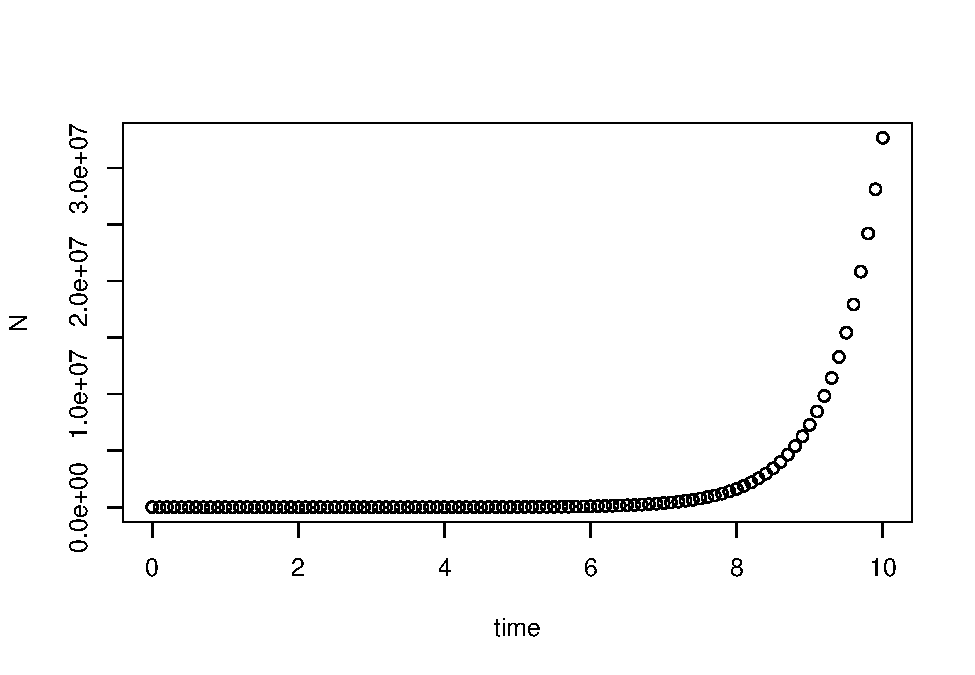
\includegraphics{bookdown-demo_files/figure-latex/unnamed-chunk-5-1.pdf}

\begin{Shaded}
\begin{Highlighting}[]
\KeywordTok{plot}\NormalTok{(N }\OperatorTok{~}\StringTok{ }\NormalTok{time, }\DataTypeTok{data =}\NormalTok{ pop_size, }\DataTypeTok{log =} \StringTok{"y"}\NormalTok{)}
\end{Highlighting}
\end{Shaded}

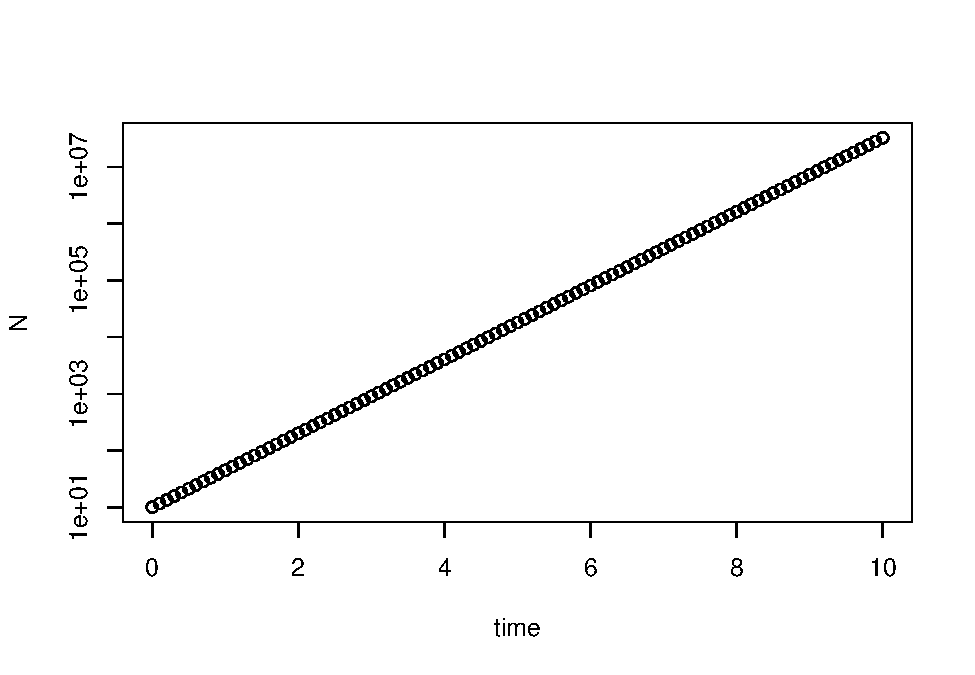
\includegraphics{bookdown-demo_files/figure-latex/unnamed-chunk-5-2.pdf}

\textbf{Part 2 - Comparing different ode solvers}
In default of \texttt{ode()}, the equations are solved by LSODA method. We can change the method by modifying the argument \texttt{method} in \texttt{ode()}.

\begin{Shaded}
\begin{Highlighting}[]
\CommentTok{###### part 2 ######}
\CommentTok{# original setting}
\NormalTok{times <-}\StringTok{ }\KeywordTok{seq}\NormalTok{(}\DecValTok{0}\NormalTok{, }\DecValTok{10}\NormalTok{, }\DataTypeTok{by =} \FloatTok{0.1}\NormalTok{)  }\CommentTok{# time steps to integrate over}
\NormalTok{state <-}\StringTok{ }\KeywordTok{c}\NormalTok{(}\DataTypeTok{N =} \DecValTok{10}\NormalTok{)  }\CommentTok{# initial population size}
\NormalTok{parms <-}\StringTok{ }\KeywordTok{c}\NormalTok{(}\DataTypeTok{r =} \FloatTok{1.5}\NormalTok{)  }\CommentTok{# intrinsic growth rate}
\CommentTok{# default: LSODA}
\NormalTok{pop_size <-}\StringTok{ }\KeywordTok{ode}\NormalTok{(}\DataTypeTok{func =}\NormalTok{ exponential_model, }\DataTypeTok{times =}\NormalTok{ times, }\DataTypeTok{y =}\NormalTok{ state, }\DataTypeTok{parms =}\NormalTok{ parms)}

\CommentTok{# Euler's method}
\NormalTok{pop_size_}\DecValTok{1}\NormalTok{ <-}\StringTok{ }\KeywordTok{ode}\NormalTok{(}\DataTypeTok{func =}\NormalTok{ exponential_model, }\DataTypeTok{times =}\NormalTok{ times, }\DataTypeTok{y =}\NormalTok{ state, }\DataTypeTok{parms =}\NormalTok{ parms, }\DataTypeTok{method =} \StringTok{"euler"}\NormalTok{)}

\CommentTok{# compare different method}
\KeywordTok{par}\NormalTok{(}\DataTypeTok{mfrow =} \KeywordTok{c}\NormalTok{(}\DecValTok{1}\NormalTok{,}\DecValTok{2}\NormalTok{))}
\KeywordTok{plot}\NormalTok{(N }\OperatorTok{~}\StringTok{ }\NormalTok{time, }\DataTypeTok{data =}\NormalTok{ pop_size, }\DataTypeTok{main =} \StringTok{"LSODA"}\NormalTok{)}
\KeywordTok{curve}\NormalTok{(state[}\DecValTok{1}\NormalTok{]}\OperatorTok{*}\KeywordTok{exp}\NormalTok{(parms[}\DecValTok{1}\NormalTok{]}\OperatorTok{*}\NormalTok{x), times[}\DecValTok{1}\NormalTok{], times[}\KeywordTok{length}\NormalTok{(times)], }\DataTypeTok{col =} \StringTok{"red"}\NormalTok{, }\DataTypeTok{add =}\NormalTok{ T) }\CommentTok{# correct curve}
\KeywordTok{plot}\NormalTok{(N }\OperatorTok{~}\StringTok{ }\NormalTok{time, }\DataTypeTok{data =}\NormalTok{ pop_size_}\DecValTok{1}\NormalTok{, }\DataTypeTok{main =} \StringTok{"Euler"}\NormalTok{)}
\KeywordTok{curve}\NormalTok{(state[}\DecValTok{1}\NormalTok{]}\OperatorTok{*}\KeywordTok{exp}\NormalTok{(parms[}\DecValTok{1}\NormalTok{]}\OperatorTok{*}\NormalTok{x), times[}\DecValTok{1}\NormalTok{], times[}\KeywordTok{length}\NormalTok{(times)], }\DataTypeTok{col =} \StringTok{"red"}\NormalTok{, }\DataTypeTok{add =}\NormalTok{ T) }\CommentTok{# correct curve}
\end{Highlighting}
\end{Shaded}

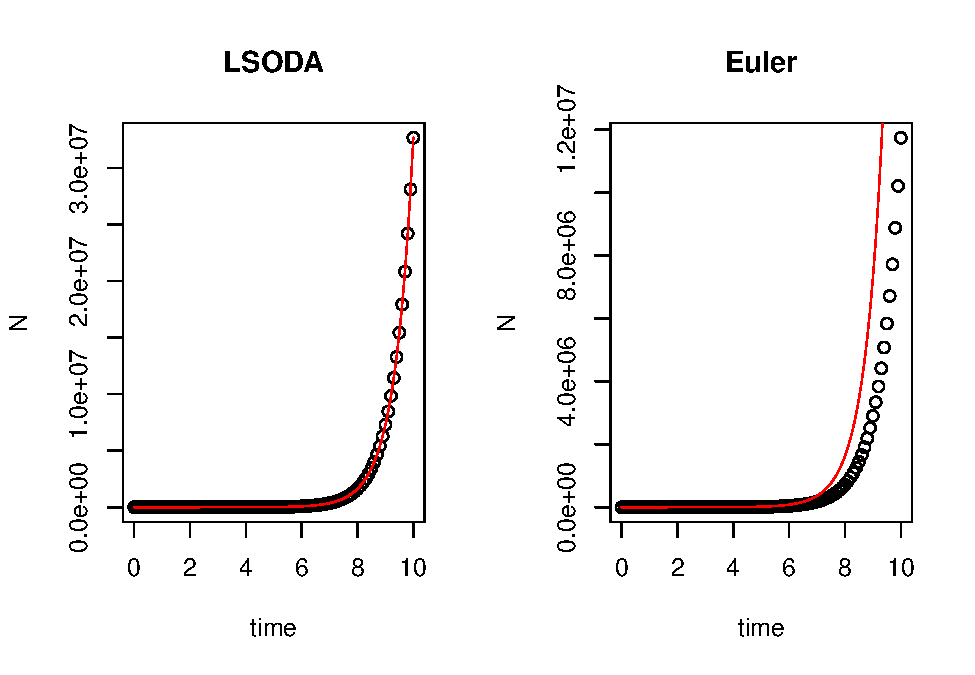
\includegraphics{bookdown-demo_files/figure-latex/unnamed-chunk-6-1.pdf}

\begin{Shaded}
\begin{Highlighting}[]
\CommentTok{# minimize the time step}
\NormalTok{times <-}\StringTok{ }\KeywordTok{seq}\NormalTok{(}\DecValTok{0}\NormalTok{, }\DecValTok{10}\NormalTok{, }\DataTypeTok{by =} \FloatTok{0.01}\NormalTok{)  }\CommentTok{# time steps to integrate over}
\NormalTok{state <-}\StringTok{ }\KeywordTok{c}\NormalTok{(}\DataTypeTok{N =} \DecValTok{10}\NormalTok{)  }\CommentTok{# initial population size}
\NormalTok{parms <-}\StringTok{ }\KeywordTok{c}\NormalTok{(}\DataTypeTok{r =} \FloatTok{1.5}\NormalTok{)  }\CommentTok{# intrinsic growth rate}
\CommentTok{# default: LSODA}
\NormalTok{pop_size <-}\StringTok{ }\KeywordTok{ode}\NormalTok{(}\DataTypeTok{func =}\NormalTok{ exponential_model, }\DataTypeTok{times =}\NormalTok{ times, }\DataTypeTok{y =}\NormalTok{ state, }\DataTypeTok{parms =}\NormalTok{ parms)}

\CommentTok{# Euler's method}
\NormalTok{pop_size_}\DecValTok{1}\NormalTok{ <-}\StringTok{ }\KeywordTok{ode}\NormalTok{(}\DataTypeTok{func =}\NormalTok{ exponential_model, }\DataTypeTok{times =}\NormalTok{ times, }\DataTypeTok{y =}\NormalTok{ state, }\DataTypeTok{parms =}\NormalTok{ parms, }\DataTypeTok{method =} \StringTok{"euler"}\NormalTok{)}

\CommentTok{# compare different method}
\KeywordTok{par}\NormalTok{(}\DataTypeTok{mfrow =} \KeywordTok{c}\NormalTok{(}\DecValTok{1}\NormalTok{,}\DecValTok{2}\NormalTok{))}
\KeywordTok{plot}\NormalTok{(N }\OperatorTok{~}\StringTok{ }\NormalTok{time, }\DataTypeTok{data =}\NormalTok{ pop_size, }\DataTypeTok{main =} \StringTok{"LSODA"}\NormalTok{)}
\KeywordTok{curve}\NormalTok{(state[}\DecValTok{1}\NormalTok{]}\OperatorTok{*}\KeywordTok{exp}\NormalTok{(parms[}\DecValTok{1}\NormalTok{]}\OperatorTok{*}\NormalTok{x), times[}\DecValTok{1}\NormalTok{], times[}\KeywordTok{length}\NormalTok{(times)], }\DataTypeTok{col =} \StringTok{"red"}\NormalTok{, }\DataTypeTok{add =}\NormalTok{ T) }\CommentTok{# correct curve}
\KeywordTok{plot}\NormalTok{(N }\OperatorTok{~}\StringTok{ }\NormalTok{time, }\DataTypeTok{data =}\NormalTok{ pop_size_}\DecValTok{1}\NormalTok{, }\DataTypeTok{main =} \StringTok{"Euler"}\NormalTok{)}
\KeywordTok{curve}\NormalTok{(state[}\DecValTok{1}\NormalTok{]}\OperatorTok{*}\KeywordTok{exp}\NormalTok{(parms[}\DecValTok{1}\NormalTok{]}\OperatorTok{*}\NormalTok{x), times[}\DecValTok{1}\NormalTok{], times[}\KeywordTok{length}\NormalTok{(times)], }\DataTypeTok{col =} \StringTok{"red"}\NormalTok{, }\DataTypeTok{add =}\NormalTok{ T) }\CommentTok{# correct curve}
\end{Highlighting}
\end{Shaded}

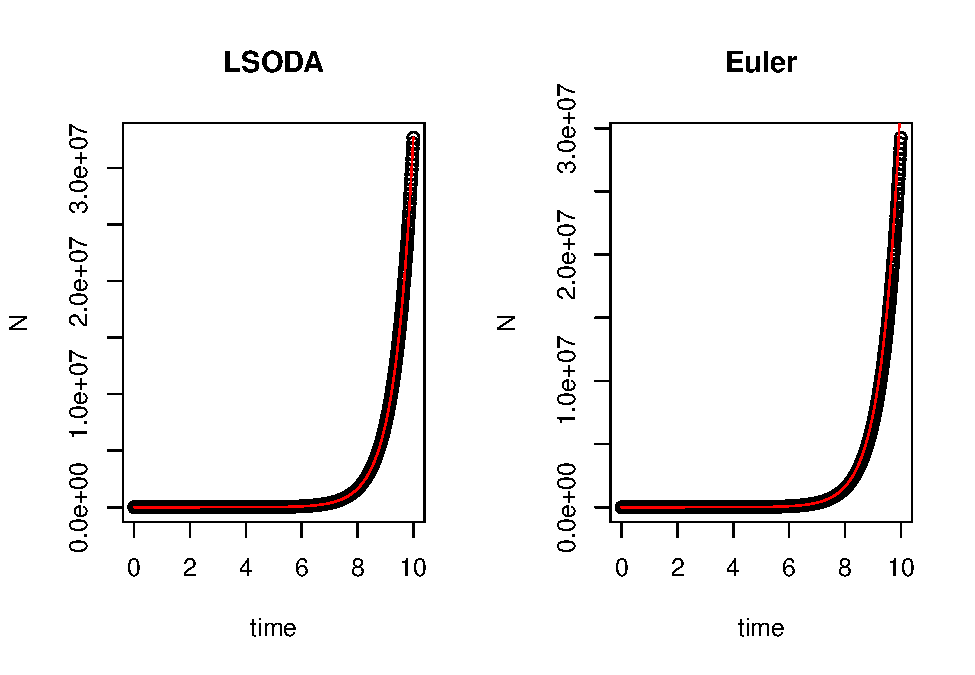
\includegraphics{bookdown-demo_files/figure-latex/unnamed-chunk-6-2.pdf}

\textbf{Part 3 - Solving exponential growth model with fluctuating growth rate}
Consider the model
\[
\frac{dN}{dt} = r(t)N \ \text{, } r(t) = \overline{r} + \sigma\sin(\omega t)
\]
where \(\overline{r}\) and \(\omega\) are constants.
The analytical solution of the ode model is
\[
N(t) = N_0\exp\{\overline{r}t - \frac{\sigma}{\omega}[\cos(\omega t) - 1]\}
\]

\begin{Shaded}
\begin{Highlighting}[]
\CommentTok{###### part 3 ######}
\CommentTok{### Model specification}
\NormalTok{exponential_model_fluc <-}\StringTok{ }\ControlFlowTok{function}\NormalTok{(times, state, parms) \{}
  \KeywordTok{with}\NormalTok{(}\KeywordTok{as.list}\NormalTok{(}\KeywordTok{c}\NormalTok{(state, parms)), \{}
\NormalTok{    dN_dt =}\StringTok{ }\NormalTok{(r_bar }\OperatorTok{+}\StringTok{ }\NormalTok{sigma}\OperatorTok{*}\KeywordTok{sin}\NormalTok{(omega}\OperatorTok{*}\NormalTok{times))}\OperatorTok{*}\NormalTok{N  }\CommentTok{# exponential growth equation}
    \KeywordTok{return}\NormalTok{(}\KeywordTok{list}\NormalTok{(}\KeywordTok{c}\NormalTok{(dN_dt)))  }\CommentTok{# return the results}
\NormalTok{  \})}
\NormalTok{\}}
\end{Highlighting}
\end{Shaded}

\begin{Shaded}
\begin{Highlighting}[]
\CommentTok{### Parameters}
\NormalTok{times <-}\StringTok{ }\KeywordTok{seq}\NormalTok{(}\DecValTok{0}\NormalTok{, }\DecValTok{10}\NormalTok{, }\DataTypeTok{by =} \FloatTok{0.1}\NormalTok{)  }\CommentTok{# time steps to integrate over}
\NormalTok{state <-}\StringTok{ }\KeywordTok{c}\NormalTok{(}\DataTypeTok{N =} \DecValTok{10}\NormalTok{)  }\CommentTok{# initial population size}
\NormalTok{parms <-}\StringTok{ }\KeywordTok{c}\NormalTok{(}\DataTypeTok{r_bar =} \FloatTok{1.5}\NormalTok{, }\DataTypeTok{sigma =} \DecValTok{5}\NormalTok{, }\DataTypeTok{omega =} \DecValTok{2}\OperatorTok{*}\NormalTok{pi)  }\CommentTok{# intrinsic growth rate}
\end{Highlighting}
\end{Shaded}

Plot \(r(t)\)

\begin{Shaded}
\begin{Highlighting}[]
\CommentTok{### Fluctuating growth rate}
\NormalTok{r =}\StringTok{ }\NormalTok{parms[}\DecValTok{1}\NormalTok{] }\OperatorTok{+}\StringTok{ }\NormalTok{parms[}\DecValTok{2}\NormalTok{]}\OperatorTok{*}\KeywordTok{sin}\NormalTok{(parms[}\DecValTok{3}\NormalTok{]}\OperatorTok{*}\NormalTok{times)}
\KeywordTok{plot}\NormalTok{(r }\OperatorTok{~}\StringTok{ }\NormalTok{times, }\DataTypeTok{type =} \StringTok{"l"}\NormalTok{)}
\end{Highlighting}
\end{Shaded}

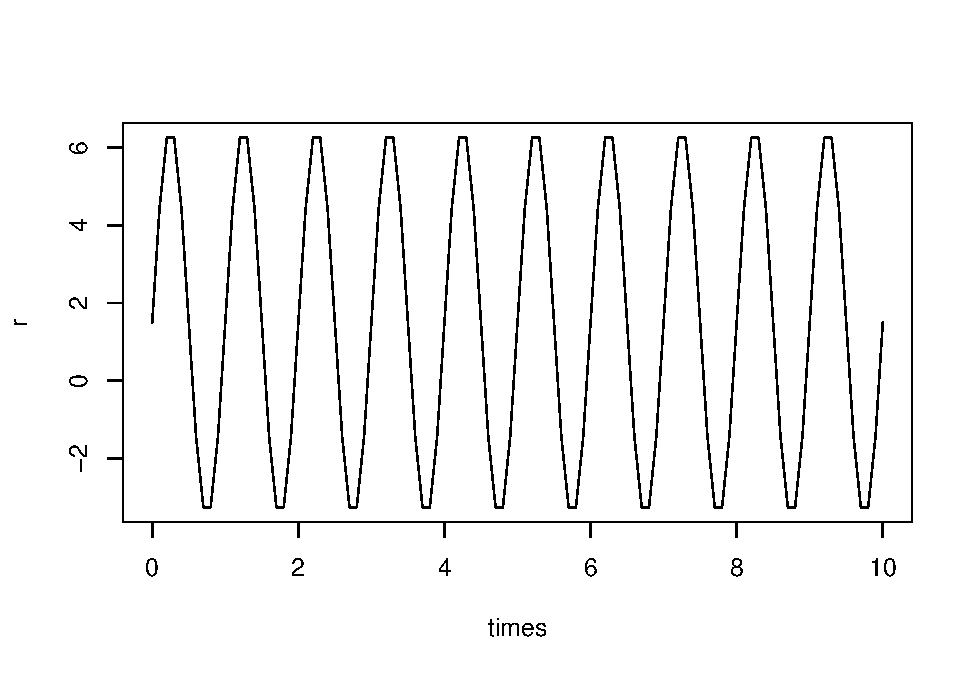
\includegraphics{bookdown-demo_files/figure-latex/unnamed-chunk-9-1.pdf}

\begin{Shaded}
\begin{Highlighting}[]
\CommentTok{### Solving model}
\NormalTok{pop_size <-}\StringTok{ }\KeywordTok{ode}\NormalTok{(}\DataTypeTok{func =}\NormalTok{ exponential_model_fluc, }\DataTypeTok{times =}\NormalTok{ times, }\DataTypeTok{y =}\NormalTok{ state, }\DataTypeTok{parms =}\NormalTok{ parms)}

\CommentTok{### Plotting}
\KeywordTok{plot}\NormalTok{(N }\OperatorTok{~}\StringTok{ }\NormalTok{times, }\DataTypeTok{data =}\NormalTok{ pop_size)}
\KeywordTok{curve}\NormalTok{(state[}\DecValTok{1}\NormalTok{]}\OperatorTok{*}\KeywordTok{exp}\NormalTok{(parms[}\DecValTok{1}\NormalTok{]}\OperatorTok{*}\NormalTok{x }\OperatorTok{-}\StringTok{ }\NormalTok{parms[}\DecValTok{2}\NormalTok{]}\OperatorTok{/}\NormalTok{parms[}\DecValTok{3}\NormalTok{]}\OperatorTok{*}\NormalTok{(}\KeywordTok{cos}\NormalTok{(parms[}\DecValTok{3}\NormalTok{]}\OperatorTok{*}\NormalTok{x) }\OperatorTok{-}\StringTok{ }\DecValTok{1}\NormalTok{)), }\DataTypeTok{add =}\NormalTok{ T, }\DataTypeTok{col =} \StringTok{"red"}\NormalTok{) }\CommentTok{# correct curve}
\end{Highlighting}
\end{Shaded}

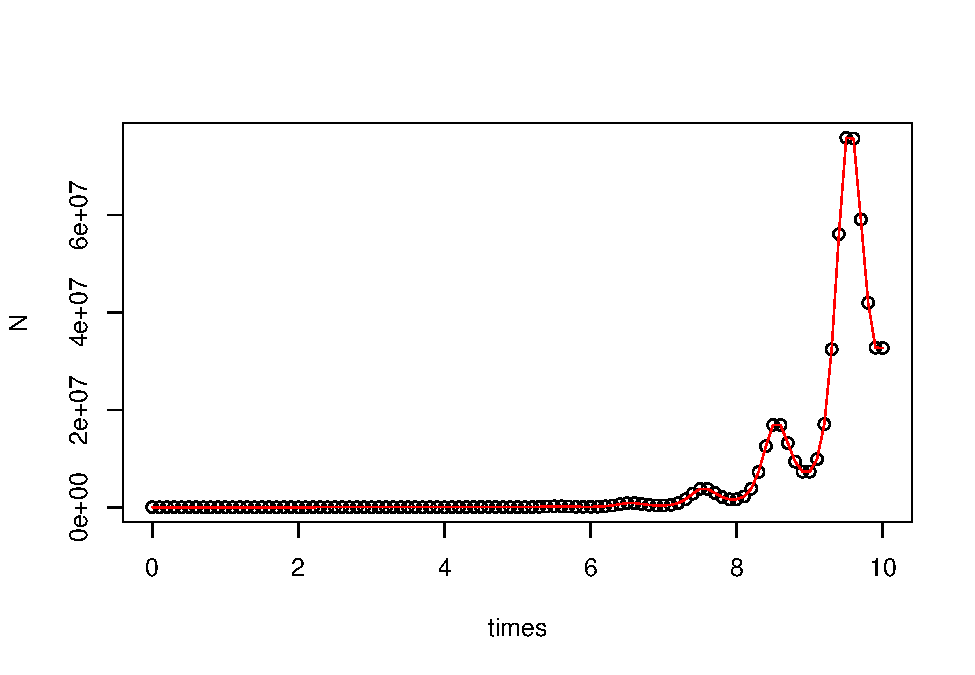
\includegraphics{bookdown-demo_files/figure-latex/unnamed-chunk-10-1.pdf}

\begin{Shaded}
\begin{Highlighting}[]
\KeywordTok{plot}\NormalTok{(N }\OperatorTok{~}\StringTok{ }\NormalTok{times, }\DataTypeTok{data =}\NormalTok{ pop_size, }\DataTypeTok{log =} \StringTok{"y"}\NormalTok{)}
\KeywordTok{curve}\NormalTok{(state[}\DecValTok{1}\NormalTok{]}\OperatorTok{*}\KeywordTok{exp}\NormalTok{(parms[}\DecValTok{1}\NormalTok{]}\OperatorTok{*}\NormalTok{x }\OperatorTok{-}\StringTok{ }\NormalTok{parms[}\DecValTok{2}\NormalTok{]}\OperatorTok{/}\NormalTok{parms[}\DecValTok{3}\NormalTok{]}\OperatorTok{*}\NormalTok{(}\KeywordTok{cos}\NormalTok{(parms[}\DecValTok{3}\NormalTok{]}\OperatorTok{*}\NormalTok{x) }\OperatorTok{-}\StringTok{ }\DecValTok{1}\NormalTok{)), }\DataTypeTok{add =}\NormalTok{ T, }\DataTypeTok{col =} \StringTok{"red"}\NormalTok{) }\CommentTok{# correct curve}
\end{Highlighting}
\end{Shaded}

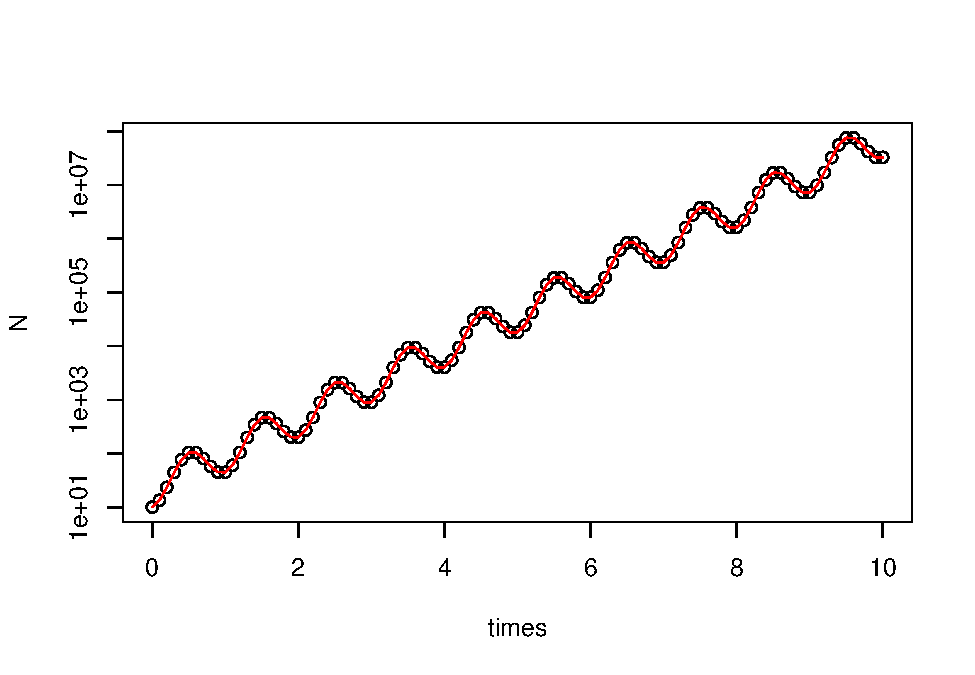
\includegraphics{bookdown-demo_files/figure-latex/unnamed-chunk-10-2.pdf}

Adjust \(\overline{r}\)

\begin{Shaded}
\begin{Highlighting}[]
\CommentTok{### Parameters}
\NormalTok{times <-}\StringTok{ }\KeywordTok{seq}\NormalTok{(}\DecValTok{0}\NormalTok{, }\DecValTok{10}\NormalTok{, }\DataTypeTok{by =} \FloatTok{0.1}\NormalTok{)  }\CommentTok{# time steps to integrate over}
\NormalTok{state <-}\StringTok{ }\KeywordTok{c}\NormalTok{(}\DataTypeTok{N =} \DecValTok{10}\NormalTok{)  }\CommentTok{# initial population size}
\NormalTok{parms <-}\StringTok{ }\KeywordTok{c}\NormalTok{(}\DataTypeTok{r_bar =} \FloatTok{0.1}\NormalTok{, }\DataTypeTok{sigma =} \DecValTok{5}\NormalTok{, }\DataTypeTok{omega =} \DecValTok{2}\OperatorTok{*}\NormalTok{pi)  }\CommentTok{# intrinsic growth rate}

\CommentTok{### Fluctuating growth rate}
\NormalTok{r =}\StringTok{ }\NormalTok{parms[}\DecValTok{1}\NormalTok{] }\OperatorTok{+}\StringTok{ }\NormalTok{parms[}\DecValTok{2}\NormalTok{]}\OperatorTok{*}\KeywordTok{sin}\NormalTok{(parms[}\DecValTok{3}\NormalTok{]}\OperatorTok{*}\NormalTok{times)}
\KeywordTok{plot}\NormalTok{(r }\OperatorTok{~}\StringTok{ }\NormalTok{times, }\DataTypeTok{type =} \StringTok{"l"}\NormalTok{)}
\end{Highlighting}
\end{Shaded}

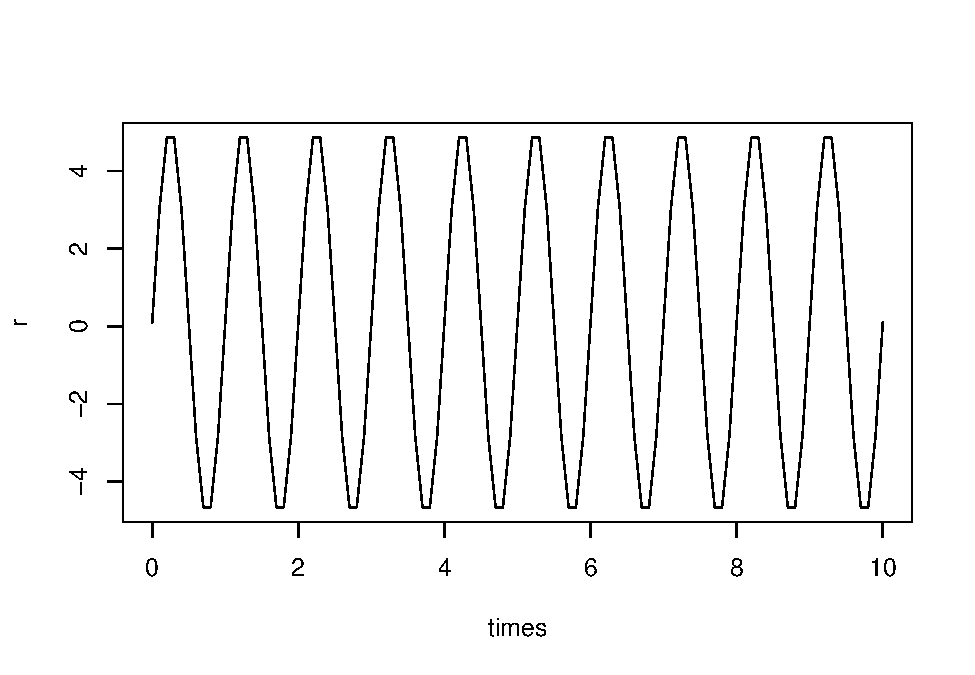
\includegraphics{bookdown-demo_files/figure-latex/unnamed-chunk-11-1.pdf}

\begin{Shaded}
\begin{Highlighting}[]
\CommentTok{### Solving model}
\NormalTok{pop_size <-}\StringTok{ }\KeywordTok{ode}\NormalTok{(}\DataTypeTok{func =}\NormalTok{ exponential_model_fluc, }\DataTypeTok{times =}\NormalTok{ times, }\DataTypeTok{y =}\NormalTok{ state, }\DataTypeTok{parms =}\NormalTok{ parms)}

\CommentTok{### Plotting}
\KeywordTok{plot}\NormalTok{(N }\OperatorTok{~}\StringTok{ }\NormalTok{times, }\DataTypeTok{data =}\NormalTok{ pop_size)}
\KeywordTok{curve}\NormalTok{(state[}\DecValTok{1}\NormalTok{]}\OperatorTok{*}\KeywordTok{exp}\NormalTok{(parms[}\DecValTok{1}\NormalTok{]}\OperatorTok{*}\NormalTok{x }\OperatorTok{-}\StringTok{ }\NormalTok{parms[}\DecValTok{2}\NormalTok{]}\OperatorTok{/}\NormalTok{parms[}\DecValTok{3}\NormalTok{]}\OperatorTok{*}\NormalTok{(}\KeywordTok{cos}\NormalTok{(parms[}\DecValTok{3}\NormalTok{]}\OperatorTok{*}\NormalTok{x) }\OperatorTok{-}\StringTok{ }\DecValTok{1}\NormalTok{)), }\DataTypeTok{add =}\NormalTok{ T, }\DataTypeTok{col =} \StringTok{"red"}\NormalTok{) }\CommentTok{# correct curve}
\end{Highlighting}
\end{Shaded}

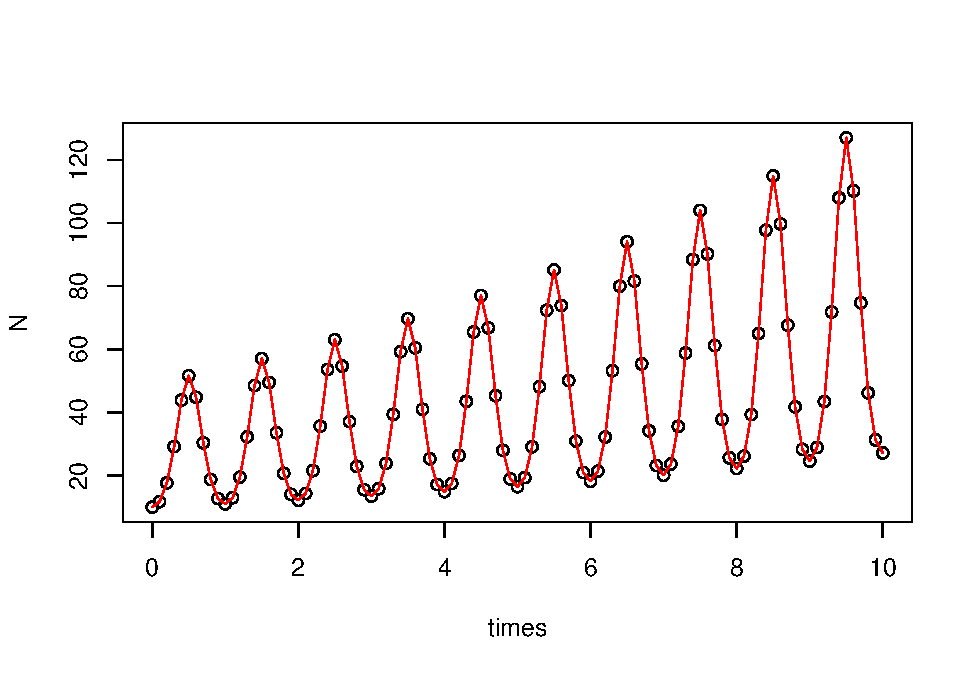
\includegraphics{bookdown-demo_files/figure-latex/unnamed-chunk-11-2.pdf}

\hypertarget{week-3---logistic-population-growth-and-stability-analysis}{%
\chapter*{Week 3 - Logistic population growth and stability analysis}\label{week-3---logistic-population-growth-and-stability-analysis}}
\addcontentsline{toc}{chapter}{Week 3 - Logistic population growth and stability analysis}

Credit to \href{https://genchanghsu.github.io/index.html}{Gen-Chang Hsu}

\hypertarget{week-4---discrete-exponential-and-logistic-models}{%
\chapter*{Week 4 - Discrete exponential and logistic models}\label{week-4---discrete-exponential-and-logistic-models}}
\addcontentsline{toc}{chapter}{Week 4 - Discrete exponential and logistic models}

\textbf{Part 1 - Model the discrete logistic population growth using for loops}
Model:
\[
N_{t+1} = N_t(1+r(1-\frac{N_t}{K}))
\]

\begin{Shaded}
\begin{Highlighting}[]
\CommentTok{### (1) Define the discrete logistic growth equation}
\NormalTok{log_fun <-}\StringTok{ }\ControlFlowTok{function}\NormalTok{(r, N, K)\{N }\OperatorTok{+}\StringTok{ }\NormalTok{r}\OperatorTok{*}\NormalTok{N}\OperatorTok{*}\NormalTok{(}\DecValTok{1}\OperatorTok{-}\NormalTok{N}\OperatorTok{/}\NormalTok{K)\}}
\end{Highlighting}
\end{Shaded}

You may modify \(r\) to see the change in stability of equilibrium \(K\).

\begin{Shaded}
\begin{Highlighting}[]
\CommentTok{### (2) Set the parameters}
\NormalTok{r <-}\StringTok{ }\FloatTok{1.8}
\NormalTok{K <-}\StringTok{ }\DecValTok{500}
\NormalTok{N0 <-}\StringTok{ }\DecValTok{10}
\NormalTok{time <-}\StringTok{ }\DecValTok{100}

\CommentTok{### (3) Use for loop to iterate over the time sequence}
\NormalTok{pop_size <-}\StringTok{ }\KeywordTok{data.frame}\NormalTok{(}\DataTypeTok{times =} \DecValTok{1}\OperatorTok{:}\NormalTok{time)}
\NormalTok{pop_size}\OperatorTok{$}\NormalTok{N[}\DecValTok{1}\NormalTok{] <-}\StringTok{ }\NormalTok{N0}
\KeywordTok{head}\NormalTok{(pop_size)}
\end{Highlighting}
\end{Shaded}

\begin{verbatim}
##   times  N
## 1     1 10
## 2     2 10
## 3     3 10
## 4     4 10
## 5     5 10
## 6     6 10
\end{verbatim}

\begin{Shaded}
\begin{Highlighting}[]
\ControlFlowTok{for}\NormalTok{(i }\ControlFlowTok{in} \DecValTok{2}\OperatorTok{:}\NormalTok{time)\{}
\NormalTok{  pop_size}\OperatorTok{$}\NormalTok{N[i] <-}\StringTok{ }\KeywordTok{log_fun}\NormalTok{(}\DataTypeTok{r =}\NormalTok{ r, }\DataTypeTok{N =}\NormalTok{ pop_size}\OperatorTok{$}\NormalTok{N[i }\OperatorTok{-}\StringTok{ }\DecValTok{1}\NormalTok{], }\DataTypeTok{K =}\NormalTok{ K)}
\NormalTok{\}}

\KeywordTok{head}\NormalTok{(pop_size)}
\end{Highlighting}
\end{Shaded}

\begin{verbatim}
##   times         N
## 1     1  10.00000
## 2     2  27.64000
## 3     3  74.64171
## 4     4 188.93980
## 5     5 400.51775
## 6     6 543.95762
\end{verbatim}

\begin{Shaded}
\begin{Highlighting}[]
\CommentTok{### (4) Population trajectory}
\KeywordTok{plot}\NormalTok{(N }\OperatorTok{~}\StringTok{ }\NormalTok{times, }\DataTypeTok{data =}\NormalTok{ pop_size, }\DataTypeTok{type =} \StringTok{"l"}\NormalTok{)}
\KeywordTok{abline}\NormalTok{(}\DataTypeTok{h =}\NormalTok{ K, }\DataTypeTok{col =} \StringTok{"red"}\NormalTok{)}
\KeywordTok{points}\NormalTok{(N }\OperatorTok{~}\StringTok{ }\NormalTok{times, }\DataTypeTok{data =}\NormalTok{ pop_size)}
\end{Highlighting}
\end{Shaded}

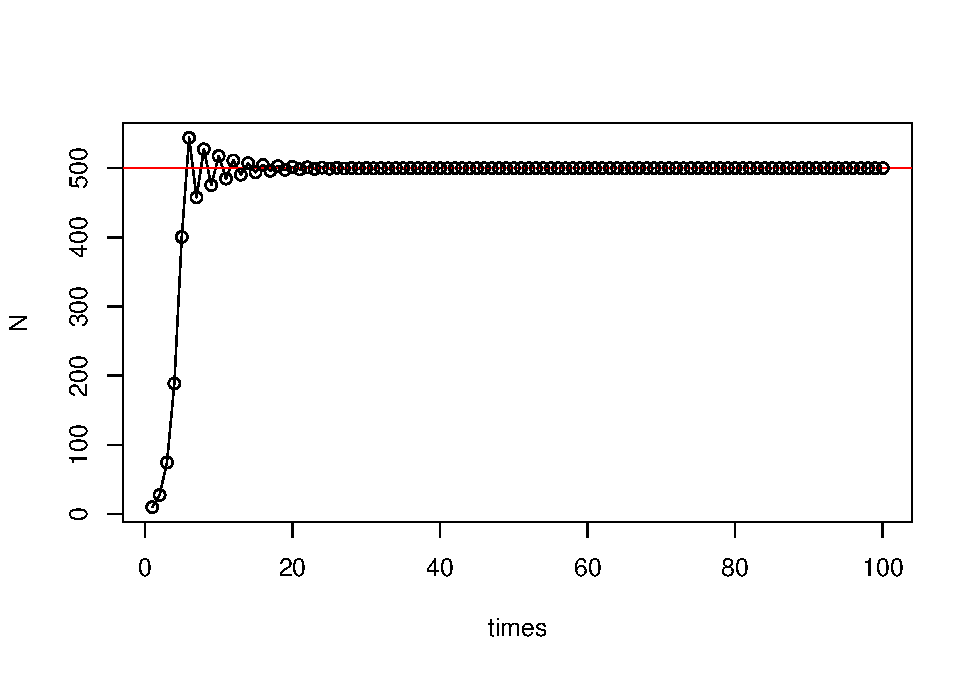
\includegraphics{bookdown-demo_files/figure-latex/unnamed-chunk-14-1.pdf}

Here is a shiny app for the discrete logistic growth model.

Credit to \href{https://genchanghsu.github.io/index.html}{Gen-Chang Hsu}

\textbf{Part 2 - Bifurcation}

\begin{Shaded}
\begin{Highlighting}[]
\CommentTok{###### Part 2: Bifurcation curve}
\CommentTok{### (1) data setting}
\CommentTok{# intrinsic growth rate sequence}
\NormalTok{r_seq <-}\StringTok{ }\KeywordTok{seq}\NormalTok{(}\DataTypeTok{from =} \FloatTok{1.8}\NormalTok{, }\DataTypeTok{to =} \DecValTok{3}\NormalTok{, }\DataTypeTok{by =} \FloatTok{0.01}\NormalTok{)}
\CommentTok{# number of sampling}
\NormalTok{N_rep <-}\StringTok{ }\DecValTok{200}

\CommentTok{# data }
\NormalTok{dat_plot <-}\StringTok{ }\KeywordTok{data.frame}\NormalTok{(}\DataTypeTok{r =} \KeywordTok{rep}\NormalTok{(r_seq, }\DataTypeTok{each =}\NormalTok{ N_rep), }\DataTypeTok{N =} \DecValTok{0}\NormalTok{)}
\KeywordTok{head}\NormalTok{(dat_plot)}
\end{Highlighting}
\end{Shaded}

\begin{verbatim}
##     r N
## 1 1.8 0
## 2 1.8 0
## 3 1.8 0
## 4 1.8 0
## 5 1.8 0
## 6 1.8 0
\end{verbatim}

\begin{Shaded}
\begin{Highlighting}[]
\CommentTok{### (2) Run the discrete logistic model}
\ControlFlowTok{for}\NormalTok{ (lo }\ControlFlowTok{in} \DecValTok{1}\OperatorTok{:}\KeywordTok{length}\NormalTok{(r_seq))\{}
\NormalTok{  log_fun <-}\StringTok{ }\ControlFlowTok{function}\NormalTok{(r, N, K)\{N }\OperatorTok{+}\StringTok{ }\NormalTok{r}\OperatorTok{*}\NormalTok{N}\OperatorTok{*}\NormalTok{(}\DecValTok{1}\OperatorTok{-}\NormalTok{N}\OperatorTok{/}\NormalTok{K)\}}

\NormalTok{  r <-}\StringTok{ }\NormalTok{r_seq[lo]}
\NormalTok{  K <-}\StringTok{ }\DecValTok{500}
\NormalTok{  N0 <-}\StringTok{ }\DecValTok{10}
\NormalTok{  time <-}\StringTok{ }\DecValTok{1000}

\NormalTok{  pop_size <-}\StringTok{ }\KeywordTok{data.frame}\NormalTok{(}\DataTypeTok{times =} \DecValTok{1}\OperatorTok{:}\NormalTok{time)}
\NormalTok{  pop_size}\OperatorTok{$}\NormalTok{N[}\DecValTok{1}\NormalTok{] <-}\StringTok{ }\NormalTok{N0}

  \ControlFlowTok{for}\NormalTok{(i }\ControlFlowTok{in} \DecValTok{2}\OperatorTok{:}\NormalTok{time)\{}
\NormalTok{    pop_size}\OperatorTok{$}\NormalTok{N[i] <-}\StringTok{ }\KeywordTok{log_fun}\NormalTok{(}\DataTypeTok{r =}\NormalTok{ r, }\DataTypeTok{N =}\NormalTok{ pop_size}\OperatorTok{$}\NormalTok{N[i }\OperatorTok{-}\StringTok{ }\DecValTok{1}\NormalTok{], }\DataTypeTok{K =}\NormalTok{ K)}
\NormalTok{  \}}

  \CommentTok{# save the data}
\NormalTok{  dat_plot}\OperatorTok{$}\NormalTok{N[(}\DecValTok{1} \OperatorTok{+}\StringTok{ }\NormalTok{(lo }\OperatorTok{-}\StringTok{ }\DecValTok{1}\NormalTok{)}\OperatorTok{*}\NormalTok{N_rep)}\OperatorTok{:}\NormalTok{(lo}\OperatorTok{*}\NormalTok{N_rep)] <-}\StringTok{ }\NormalTok{pop_size}\OperatorTok{$}\NormalTok{N[(}\KeywordTok{nrow}\NormalTok{(pop_size) }\OperatorTok{-}\StringTok{ }\NormalTok{N_rep }\OperatorTok{+}\StringTok{ }\DecValTok{1}\NormalTok{)}\OperatorTok{:}\KeywordTok{nrow}\NormalTok{(pop_size)]}
\NormalTok{\}}

\KeywordTok{plot}\NormalTok{(N }\OperatorTok{~}\StringTok{ }\NormalTok{r, }\DataTypeTok{data =}\NormalTok{ dat_plot, }\DataTypeTok{cex =} \FloatTok{0.7}\NormalTok{, }\DataTypeTok{pch =} \DecValTok{20}\NormalTok{)}
\end{Highlighting}
\end{Shaded}

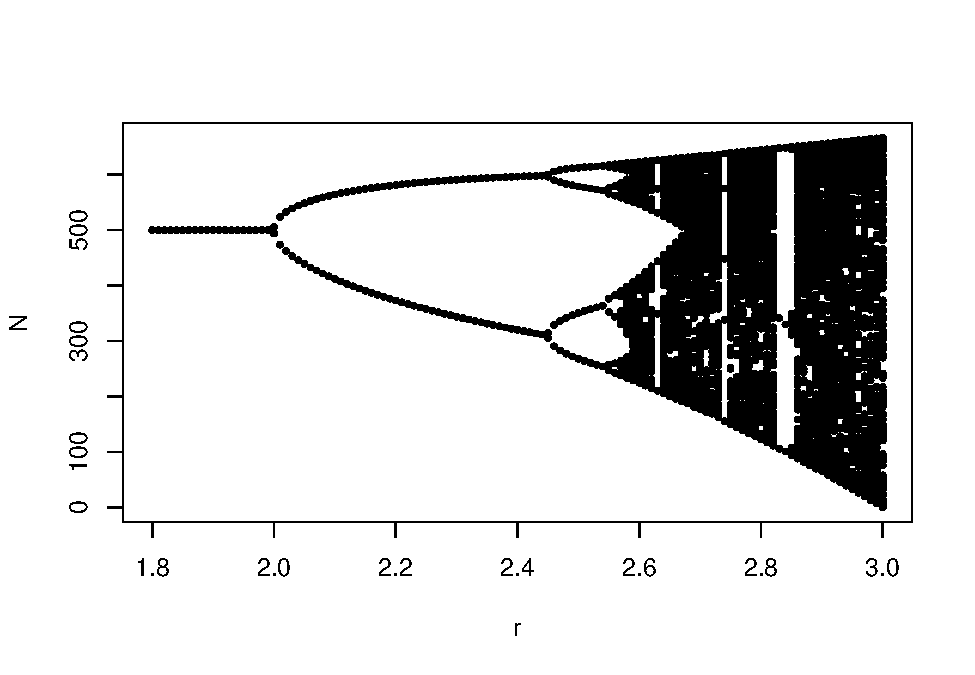
\includegraphics{bookdown-demo_files/figure-latex/unnamed-chunk-16-1.pdf}

\hypertarget{week-5---age-structure-population-model}{%
\chapter*{Week 5 - Age-structure population model}\label{week-5---age-structure-population-model}}
\addcontentsline{toc}{chapter}{Week 5 - Age-structure population model}

In this lab section, we will analyze a Leslie matrix using for loops and matrix algebra, compare the results with those obtained via eigen-analysis, and visualize the population dynamics and age distribution.

\textbf{Part 1 - Visualizing stable age distribution}

For any diagonalizable n-by-n matrix \(M\) with only one dominant eigenvalue, and for any n-by-1 vector \(v\), \(M^tv\) will shift to the same direction with the eigenvector of \(M\) corresponding to the dominant eigenvalue when \(t\) is large. Here, we visualize this fact numerically.

\begin{Shaded}
\begin{Highlighting}[]
\KeywordTok{library}\NormalTok{(ggplot2)}
\KeywordTok{set.seed}\NormalTok{(}\DecValTok{1234}\NormalTok{)}
\NormalTok{MAT <-}\StringTok{ }\KeywordTok{matrix}\NormalTok{(}\KeywordTok{rnorm}\NormalTok{(}\DecValTok{25}\NormalTok{), }\DataTypeTok{ncol =} \DecValTok{5}\NormalTok{, }\DataTypeTok{nrow =} \DecValTok{5}\NormalTok{)}
\KeywordTok{abs}\NormalTok{(}\KeywordTok{eigen}\NormalTok{(MAT)}\OperatorTok{$}\NormalTok{values) }\CommentTok{# check only one dominant eigenvalue}
\end{Highlighting}
\end{Shaded}

\begin{verbatim}
## [1] 2.2734833 1.6266143 0.6187862 0.6187862 0.3970850
\end{verbatim}

\begin{Shaded}
\begin{Highlighting}[]
\NormalTok{eig_vec1 <-}\StringTok{ }\KeywordTok{as.numeric}\NormalTok{(}\KeywordTok{eigen}\NormalTok{(MAT)}\OperatorTok{$}\NormalTok{vector[, }\DecValTok{1}\NormalTok{])}
\NormalTok{v <-}\StringTok{ }\KeywordTok{rnorm}\NormalTok{(}\DecValTok{5}\NormalTok{)}
\NormalTok{time <-}\StringTok{ }\DecValTok{15}

\NormalTok{dat_v <-}\StringTok{ }\KeywordTok{data.frame}\NormalTok{(}\KeywordTok{matrix}\NormalTok{(}\DataTypeTok{ncol =} \DecValTok{5}\NormalTok{, }\DataTypeTok{nrow =}\NormalTok{ time))}
\NormalTok{dat_v[}\DecValTok{1}\NormalTok{, ] <-}\StringTok{ }\NormalTok{v}
\ControlFlowTok{for}\NormalTok{(i }\ControlFlowTok{in} \DecValTok{2}\OperatorTok{:}\NormalTok{time)\{}
\NormalTok{  dat_v[i, ] <-}\StringTok{ }\NormalTok{MAT }\OperatorTok\StringTok{ }\KeywordTok{t}\NormalTok{(dat_v[i}\DecValTok{-1}\NormalTok{, ])}
\NormalTok{\}}

\CommentTok{# Remake data for gganimate}
\NormalTok{dat <-}\StringTok{ }\KeywordTok{data.frame}\NormalTok{(}\DataTypeTok{X1 =} \DecValTok{0}\NormalTok{, }\DataTypeTok{X2 =} \DecValTok{0}\NormalTok{, }\DataTypeTok{Time =} \DecValTok{1}\NormalTok{)}
\ControlFlowTok{for}\NormalTok{(i }\ControlFlowTok{in} \DecValTok{1}\OperatorTok{:}\NormalTok{time)\{}
\NormalTok{  dat <-}\StringTok{ }\KeywordTok{rbind}\NormalTok{(dat, }\KeywordTok{data.frame}\NormalTok{(dat_v[i,}\DecValTok{1}\OperatorTok{:}\DecValTok{2}\NormalTok{] }\OperatorTok{/}\StringTok{ }\KeywordTok{sqrt}\NormalTok{(}\KeywordTok{sum}\NormalTok{(dat_v[i,}\DecValTok{1}\OperatorTok{:}\DecValTok{2}\NormalTok{]}\OperatorTok{^}\DecValTok{2}\NormalTok{)) }\OperatorTok{*}\StringTok{ }\NormalTok{i, }\DataTypeTok{Time =}\NormalTok{ i))}
\NormalTok{  dat <-}\StringTok{ }\KeywordTok{rbind}\NormalTok{(dat, }\KeywordTok{c}\NormalTok{(}\DecValTok{0}\NormalTok{,}\DecValTok{0}\NormalTok{, i}\OperatorTok{+}\DecValTok{1}\NormalTok{))}
\NormalTok{\}}
\NormalTok{dat <-}\StringTok{ }\NormalTok{dat[}\OperatorTok{-}\KeywordTok{nrow}\NormalTok{(dat), ]}


\KeywordTok{ggplot}\NormalTok{(dat, }\KeywordTok{aes}\NormalTok{(X1, X2, }\DataTypeTok{color =}\NormalTok{ Time)) }\OperatorTok{+}
\StringTok{  }\KeywordTok{geom_path}\NormalTok{(}\DataTypeTok{arrow =} \KeywordTok{arrow}\NormalTok{(}\DataTypeTok{length =} \KeywordTok{unit}\NormalTok{(}\FloatTok{0.55}\NormalTok{, }\StringTok{"cm"}\NormalTok{))) }\OperatorTok{+}\StringTok{ }
\StringTok{  }\KeywordTok{geom_abline}\NormalTok{(}\DataTypeTok{intercept =} \DecValTok{0}\NormalTok{, }
              \DataTypeTok{slope =}\NormalTok{ eig_vec1[}\DecValTok{2}\NormalTok{]}\OperatorTok{/}\NormalTok{eig_vec1[}\DecValTok{1}\NormalTok{], }
              \DataTypeTok{color =} \StringTok{"red"}\NormalTok{, }
              \DataTypeTok{linetype =} \StringTok{"dashed"}\NormalTok{) }\CommentTok{# red dashed eigenvector}
\end{Highlighting}
\end{Shaded}

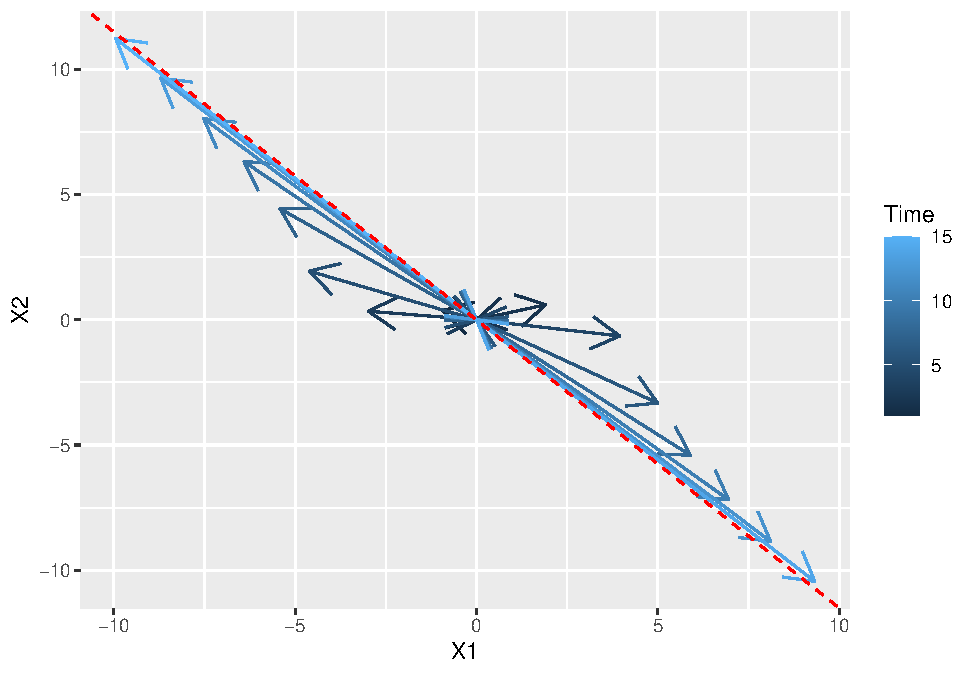
\includegraphics{bookdown-demo_files/figure-latex/unnamed-chunk-17-1.pdf}

\textbf{Part 2 - Analyzing Leslie matrix}

Consider an age-strutured population model
\[
n_{t} = L^tn_0
\]
where \(L\) is a Leslie matrix and \(n_t = (n_{1,t}, n_{2,t}, n_{3,t})\) is the population sizes with three different ages in time \(t\).

\begin{Shaded}
\begin{Highlighting}[]
\CommentTok{### Leslie matrix and initial age classes}
\NormalTok{leslie <-}\StringTok{ }\KeywordTok{matrix}\NormalTok{(}\DataTypeTok{data =} \KeywordTok{c}\NormalTok{(}\DecValTok{0}\NormalTok{, }\DecValTok{1}\NormalTok{, }\DecValTok{5}\NormalTok{,}
                          \FloatTok{0.5}\NormalTok{, }\DecValTok{0}\NormalTok{, }\DecValTok{0}\NormalTok{,}
                          \DecValTok{0}\NormalTok{, }\FloatTok{0.3}\NormalTok{, }\DecValTok{0}\NormalTok{),}
                      \DataTypeTok{nrow =} \DecValTok{3}\NormalTok{,}
                      \DataTypeTok{ncol =} \DecValTok{3}\NormalTok{,}
                      \DataTypeTok{byrow =}\NormalTok{ T)}

\NormalTok{N0 <-}\StringTok{ }\KeywordTok{c}\NormalTok{(}\DecValTok{10}\NormalTok{, }\DecValTok{0}\NormalTok{, }\DecValTok{0}\NormalTok{)}

\CommentTok{### for loop and matrix algebra}
\NormalTok{time <-}\StringTok{ }\DecValTok{50}
\NormalTok{pop_size <-}\StringTok{ }\KeywordTok{data.frame}\NormalTok{(}\DataTypeTok{Age1 =} \DecValTok{0}\NormalTok{,}
                       \DataTypeTok{Age2 =} \DecValTok{0}\NormalTok{,}
                       \DataTypeTok{Age3 =} \DecValTok{0}\NormalTok{)}
\NormalTok{pop_size[}\DecValTok{1}\NormalTok{, ] <-}\StringTok{ }\NormalTok{N0}

\ControlFlowTok{for}\NormalTok{ (i }\ControlFlowTok{in} \DecValTok{2}\OperatorTok{:}\NormalTok{time) \{}
  \CommentTok{# Matrix multiplication}
\NormalTok{  pop_size[i, ] <-}\StringTok{ }\NormalTok{leslie }\OperatorTok\StringTok{ }\KeywordTok{t}\NormalTok{(pop_size[i}\DecValTok{-1}\NormalTok{, ])}
\NormalTok{\}}

\CommentTok{# Total abundance}
\NormalTok{pop_size}\OperatorTok{$}\NormalTok{N <-}\StringTok{ }\KeywordTok{rowSums}\NormalTok{(pop_size)}

\KeywordTok{head}\NormalTok{(pop_size)}
\end{Highlighting}
\end{Shaded}

\begin{verbatim}
##   Age1 Age2  Age3      N
## 1 10.0 0.00 0.000 10.000
## 2  0.0 5.00 0.000  5.000
## 3  5.0 0.00 1.500  6.500
## 4  7.5 2.50 0.000 10.000
## 5  2.5 3.75 0.750  7.000
## 6  7.5 1.25 1.125  9.875
\end{verbatim}

\begin{Shaded}
\begin{Highlighting}[]
\KeywordTok{plot}\NormalTok{(}\KeywordTok{c}\NormalTok{(}\DecValTok{1}\NormalTok{,time), }\KeywordTok{c}\NormalTok{(}\DecValTok{0}\NormalTok{,}\DecValTok{265}\NormalTok{), }\DataTypeTok{type =} \StringTok{"n"}\NormalTok{, }\DataTypeTok{xlab =} \StringTok{"time"}\NormalTok{, }\DataTypeTok{ylab =} \StringTok{"pop_size"}\NormalTok{)}
\KeywordTok{lines}\NormalTok{(}\DecValTok{1}\OperatorTok{:}\NormalTok{time , pop_size}\OperatorTok{$}\NormalTok{Age1, }\DataTypeTok{col =} \StringTok{"red"}\NormalTok{)}
\KeywordTok{lines}\NormalTok{(}\DecValTok{1}\OperatorTok{:}\NormalTok{time , pop_size}\OperatorTok{$}\NormalTok{Age2, }\DataTypeTok{col =} \StringTok{"blue"}\NormalTok{)}
\KeywordTok{lines}\NormalTok{(}\DecValTok{1}\OperatorTok{:}\NormalTok{time , pop_size}\OperatorTok{$}\NormalTok{Age3, }\DataTypeTok{col =} \StringTok{"green"}\NormalTok{)}
\KeywordTok{legend}\NormalTok{(}\StringTok{"topleft"}\NormalTok{,}
       \DataTypeTok{legend =} \KeywordTok{c}\NormalTok{(}\StringTok{"Age1"}\NormalTok{, }\StringTok{"Age2"}\NormalTok{, }\StringTok{"Age3"}\NormalTok{),}
       \DataTypeTok{col =} \KeywordTok{c}\NormalTok{(}\StringTok{"red"}\NormalTok{, }\StringTok{"blue"}\NormalTok{, }\StringTok{"green"}\NormalTok{),}
       \DataTypeTok{lty =} \DecValTok{1}\NormalTok{)}
\end{Highlighting}
\end{Shaded}

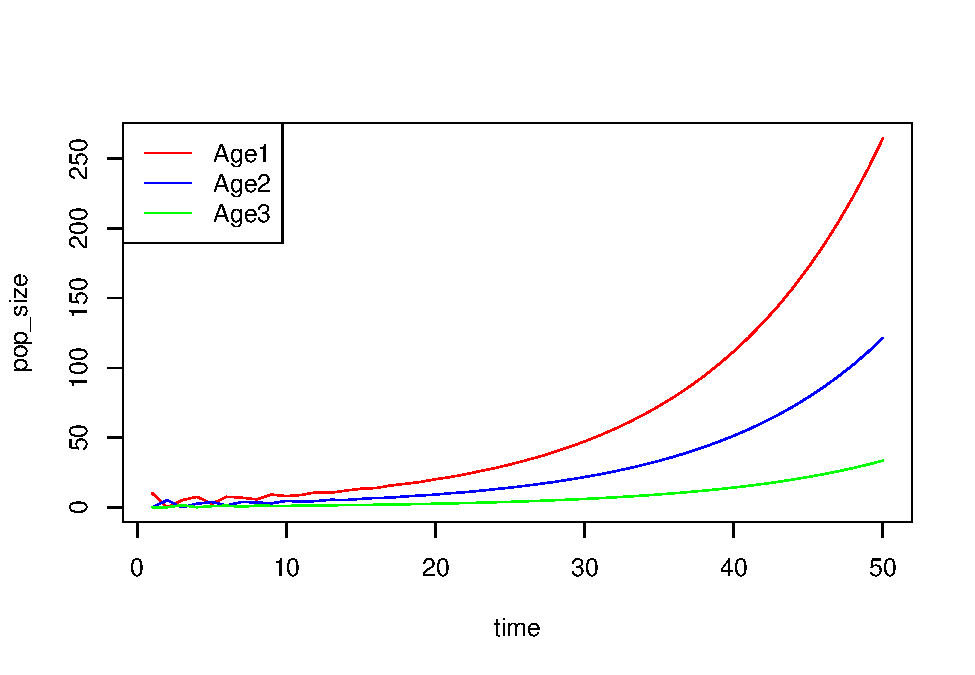
\includegraphics{bookdown-demo_files/figure-latex/unnamed-chunk-18-1.pdf}

By the derivation in the class, the asymptotic population sizes can be approximated by
\[
n_t \approx c\cdot \lambda_1^t\cdot u_1
\]
where \(c\) is a constant, \(\lambda_1\) is the dominant eigenvalue and \(u_1\) is the corresponding eigenvector. Hence, with the long-term dynamics, the population grows at a rate \(\lambda_1\) and with the age distribution \(u_1\). Here, we check this fact numerically.

\begin{Shaded}
\begin{Highlighting}[]
\CommentTok{### Asymptotic growth rate and stable age distribution}

\NormalTok{asymptotic_growth <-}\StringTok{ }\NormalTok{pop_size}\OperatorTok{$}\NormalTok{N[time]}\OperatorTok{/}\NormalTok{pop_size}\OperatorTok{$}\NormalTok{N[time}\DecValTok{-1}\NormalTok{]}
\NormalTok{asymptotic_growth}
\end{Highlighting}
\end{Shaded}

\begin{verbatim}
## [1] 1.089992
\end{verbatim}

\begin{Shaded}
\begin{Highlighting}[]
\NormalTok{age_distribution <-}\StringTok{ }\NormalTok{pop_size[time, }\DecValTok{1}\OperatorTok{:}\DecValTok{3}\NormalTok{]}\OperatorTok{/}\KeywordTok{sum}\NormalTok{(pop_size[time, }\DecValTok{1}\OperatorTok{:}\DecValTok{3}\NormalTok{])}
\NormalTok{age_distribution}
\end{Highlighting}
\end{Shaded}

\begin{verbatim}
##         Age1      Age2       Age3
## 50 0.6309262 0.2894167 0.07965713
\end{verbatim}

\begin{Shaded}
\begin{Highlighting}[]
\CommentTok{### Eigen-analysis of the Leslie matrix}
\NormalTok{EIGEN <-}\StringTok{ }\KeywordTok{eigen}\NormalTok{(leslie)}
\NormalTok{EIGEN}
\end{Highlighting}
\end{Shaded}

\begin{verbatim}
## eigen() decomposition
## $values
## [1]  1.0899905+0.0000000i -0.5449953+0.6253475i -0.5449953-0.6253475i
## 
## $vectors
##              [,1]                  [,2]                  [,3]
## [1,] 0.9030054+0i  0.8418972+0.0000000i  0.8418972+0.0000000i
## [2,] 0.4142263+0i -0.3334136-0.3825709i -0.3334136+0.3825709i
## [3,] 0.1140082+0i -0.0250833+0.1818099i -0.0250833-0.1818099i
\end{verbatim}

\begin{Shaded}
\begin{Highlighting}[]
\KeywordTok{abs}\NormalTok{(EIGEN}\OperatorTok{$}\NormalTok{values[}\DecValTok{1}\NormalTok{]) }\CommentTok{# dominant eigenvalue}
\end{Highlighting}
\end{Shaded}

\begin{verbatim}
## [1] 1.089991
\end{verbatim}

\begin{Shaded}
\begin{Highlighting}[]
\KeywordTok{as.numeric}\NormalTok{(EIGEN}\OperatorTok{$}\NormalTok{vectors[, }\DecValTok{1}\NormalTok{] }\OperatorTok{/}\StringTok{ }\KeywordTok{sum}\NormalTok{(EIGEN}\OperatorTok{$}\NormalTok{vectors[, }\DecValTok{1}\NormalTok{])) }\CommentTok{# corresponding eigenvector}
\end{Highlighting}
\end{Shaded}

\begin{verbatim}
## [1] 0.63092527 0.28941777 0.07965696
\end{verbatim}

The asymptotic growth rate and stable age distribution obtained from for loops and eigen-analysis are similar.

\textbf{Part 3 - In-class exercise: Analyzing population matrix of common teasel}

\href{https://en.wikipedia.org/wiki/Dipsacus_fullonum}{Common teasel (\emph{Dipsacus sylvestris})} is a herbaceous plant commonly found in abandoned fields and meadows in North America. It has a complex life cycle consisting of various stages. The seeds may lie dormant for one or two years. Seeds that germinate form small rosettes, which will gradually transit into medium and eventually large rosettes. These rosettes (all three sizes) may remain in the same stage for years before entering the next stage. After undergoing vernalization, large (and a few medium) rosettes will form stalks and flower in the upcoming summer, set seeds once, and die. Occasionally, the flowering plants will produce seeds that directly germinate into small/medium/large rosettes without entering dormancy.

Here is a transition diagram for the teasel. Please convert this diagram into a stage-based transition matrix (Lefkovitch matrix) and derive the asymptotic growth rate \(\lambda\) in R.

\textbf{Part 4 - COM(P)ADRE: A global database of population matrices}

\href{https://compadre-db.org/ExploreDatabase}{COM(P)ADRE} is an online repository containing matrix population models on hundreds of plants, animals, algae, fungi, bacteria, and viruses around the world, as well as their associated metadata. Take a look at the website: You will be exploring the population dynamics of a species (of your choice) in your assignment!

\hypertarget{week-6---metapopulations-and-patch-occupancy-models}{%
\chapter*{Week 6 - Metapopulations and patch occupancy models}\label{week-6---metapopulations-and-patch-occupancy-models}}
\addcontentsline{toc}{chapter}{Week 6 - Metapopulations and patch occupancy models}

Plants can condition nearby soil microbial communities, which will in turn influence the performance of subsequent colonizing plants. The soil beneath plant communities are therefore a mosaic with different cultivation histories. Po-Ju wants to understand how plant demographic rates (i.e., colonization and mortality rate) and microbial dynamics (i.e., the conditioning and decay rate of microbial communities) affect the percentage of different soil types in natural forests. As a starting point, Po-Ju builds a one-species patch occupancy model to track the dynamics of different types of plant-soil combination.

In this model, he characterizes sites by their plant-soil microbe state, using the notation \(P_{ij}\) to indicate sites that are now occupied by plant species \(i\) but have soil microbes state \(j\). Here, as a single species model, \(i\) can be 0 or \(A\), representing uncolonized sites or sites colonized by plant \(A\), respectively. Similarly, \(j\) can be 0 or \(A\), indicating sites without recent plant conditioning history or sites conditioned by plant \(A\), respectively. In summary:

\begin{enumerate}
\def\labelenumi{\arabic{enumi}.}
\tightlist
\item
  \(P_{00}\) represents uncolonized and unconditioned sites
\item
  \(P_{A0}\) represents cites colonized by plant \(A\) but the soil is yet to be conditioned
\item
  \(P_{AA}\) represents plant \(A\) colonizing a site with plant-\(A\)-specific microbial community
\item
  \(P_{0A}\) represents sites that are currently unoccupied but have soil microbes that were associated with plant \(A\)
\end{enumerate}

At the landscape scale, \(P_{ij}\) represents the proportion of sites belonging to a particular plant-soil microbe state, and its dynamics, \(\frac {dP_{ij}}{dt}\), summarizes the processes of plant colonization and death. The transitions between different plant-soil microbe states can be described by the following figure.

Here, \(P_{00}\) can be colonized by plant \(A\) when propagules arrive (per capita rate \(r_{A}\)), transitioning the state from \(P_{00}\) to \(P_{A0}\). Plants may die, with rate \(m_{A}\), before conditioning the soil (i.e., transition from \(P_{A0}\) back to \(P_{00}\)), or may successfully condition the soil with rate \(c_{A}\) (i.e., transition from \(P_{A0}\) to \(P_{AA}\)). After plants within the state \(P_{AA}\) die, a site with microbial legacy is left behind, denoted as \(P_{0A}\). These empty sites can be recolonized (i.e., transition from \(P_{0A}\) back to \(P_{AA}\)) with rates affected by the microbial legacy effect, \(\alpha\). Finally, the microbial community within the soil may decay to unconditioned state with rate \(d_{A}\), transitioning the state from \(P_{0A}\) to \(P_{00}\).

In this lab, we are going to model the dynamics of this plant-soil system. We will start by converting the flow diagram into a set of differential equations and then solve them numerically using the package \texttt{deSolve}.

\begin{Shaded}
\begin{Highlighting}[]
\KeywordTok{library}\NormalTok{(deSolve)}
\KeywordTok{library}\NormalTok{(ggplot2)}
\KeywordTok{library}\NormalTok{(tidyr)}


\CommentTok{### Model specification}
\NormalTok{PSF <-}\StringTok{ }\ControlFlowTok{function}\NormalTok{(times, state, parms) \{}
  \KeywordTok{with}\NormalTok{(}\KeywordTok{as.list}\NormalTok{(}\KeywordTok{c}\NormalTok{(state, parms)), \{}
\NormalTok{    dP00_dt =}\StringTok{ }\NormalTok{P0A}\OperatorTok{*}\NormalTok{dA }\OperatorTok{+}\StringTok{ }\NormalTok{PA0}\OperatorTok{*}\NormalTok{mA }\OperatorTok{-}\StringTok{ }\NormalTok{P00}\OperatorTok{*}\NormalTok{(PA0 }\OperatorTok{+}\StringTok{ }\NormalTok{PAA)}\OperatorTok{*}\NormalTok{rA}
\NormalTok{    dPA0_dt =}\StringTok{ }\NormalTok{P00}\OperatorTok{*}\NormalTok{(PA0 }\OperatorTok{+}\StringTok{ }\NormalTok{PAA)}\OperatorTok{*}\NormalTok{rA }\OperatorTok{-}\StringTok{ }\NormalTok{PA0}\OperatorTok{*}\NormalTok{mA }\OperatorTok{-}\StringTok{ }\NormalTok{PA0}\OperatorTok{*}\NormalTok{cA}
\NormalTok{    dPAA_dt =}\StringTok{ }\NormalTok{PA0}\OperatorTok{*}\NormalTok{cA }\OperatorTok{-}\StringTok{ }\NormalTok{PAA}\OperatorTok{*}\NormalTok{mA }\OperatorTok{+}\StringTok{ }\NormalTok{P0A}\OperatorTok{*}\NormalTok{(PA0 }\OperatorTok{+}\StringTok{ }\NormalTok{PAA)}\OperatorTok{*}\NormalTok{rA}\OperatorTok{*}\NormalTok{alpha}
\NormalTok{    dP0A_dt =}\StringTok{ }\NormalTok{PAA}\OperatorTok{*}\NormalTok{mA }\OperatorTok{-}\StringTok{ }\NormalTok{P0A}\OperatorTok{*}\NormalTok{(PA0 }\OperatorTok{+}\StringTok{ }\NormalTok{PAA)}\OperatorTok{*}\NormalTok{rA}\OperatorTok{*}\NormalTok{alpha }\OperatorTok{-}\StringTok{ }\NormalTok{P0A}\OperatorTok{*}\NormalTok{dA}

    \KeywordTok{return}\NormalTok{(}\KeywordTok{list}\NormalTok{(}\KeywordTok{c}\NormalTok{(dP00_dt, dPA0_dt, dPAA_dt, dP0A_dt)))}
\NormalTok{  \})}
\NormalTok{\}}

\CommentTok{### Model parameters}
\NormalTok{times <-}\StringTok{ }\KeywordTok{seq}\NormalTok{(}\DecValTok{0}\NormalTok{, }\DecValTok{20}\NormalTok{, }\DataTypeTok{by =} \FloatTok{0.1}\NormalTok{)}
\NormalTok{state <-}\StringTok{ }\KeywordTok{c}\NormalTok{(}\DataTypeTok{P00 =} \FloatTok{0.25}\NormalTok{, }\DataTypeTok{PA0 =} \FloatTok{0.25}\NormalTok{, }\DataTypeTok{PAA =} \FloatTok{0.25}\NormalTok{, }\DataTypeTok{P0A =} \FloatTok{0.25}\NormalTok{)}
\NormalTok{parms <-}\StringTok{ }\KeywordTok{c}\NormalTok{(}\DataTypeTok{rA =} \FloatTok{0.5}\NormalTok{, }\DataTypeTok{mA =} \FloatTok{0.1}\NormalTok{, }\DataTypeTok{cA =} \FloatTok{0.5}\NormalTok{, }\DataTypeTok{dA =} \FloatTok{0.4}\NormalTok{, }\DataTypeTok{alpha =} \FloatTok{0.7}\NormalTok{)}

\CommentTok{### ODE solver}
\NormalTok{pop_size <-}\StringTok{ }\KeywordTok{ode}\NormalTok{(}\DataTypeTok{func =}\NormalTok{ PSF, }\DataTypeTok{times =}\NormalTok{ times, }\DataTypeTok{y =}\NormalTok{ state, }\DataTypeTok{parms =}\NormalTok{ parms)}

\CommentTok{# take a look at the results}
\KeywordTok{head}\NormalTok{(pop_size)}
\end{Highlighting}
\end{Shaded}

\begin{verbatim}
##      time       P00       PA0       PAA       P0A
## [1,]  0.0 0.2500000 0.2500000 0.2500000 0.2500000
## [2,]  0.1 0.2558649 0.2416153 0.2640144 0.2385055
## [3,]  0.2 0.2609930 0.2339241 0.2773399 0.2277430
## [4,]  0.3 0.2654349 0.2268709 0.2900255 0.2176687
## [5,]  0.4 0.2692386 0.2204039 0.3021162 0.2082413
## [6,]  0.5 0.2724484 0.2144756 0.3136533 0.1994227
\end{verbatim}

\begin{Shaded}
\begin{Highlighting}[]
\KeywordTok{tail}\NormalTok{(pop_size)}
\end{Highlighting}
\end{Shaded}

\begin{verbatim}
##        time       P00        PA0       PAA       P0A
## [196,] 19.5 0.1283001 0.08252532 0.6866677 0.1025070
## [197,] 19.6 0.1282914 0.08250852 0.6866865 0.1025136
## [198,] 19.7 0.1282832 0.08249240 0.6867045 0.1025199
## [199,] 19.8 0.1282754 0.08247693 0.6867217 0.1025260
## [200,] 19.9 0.1282679 0.08246208 0.6867382 0.1025319
## [201,] 20.0 0.1282608 0.08244784 0.6867539 0.1025375
\end{verbatim}

\begin{Shaded}
\begin{Highlighting}[]
\CommentTok{### Visualization I}
\NormalTok{pop_size }\OperatorTok
\StringTok{  }\KeywordTok{as.data.frame}\NormalTok{() }\OperatorTok
\StringTok{  }\KeywordTok{gather}\NormalTok{(}\DataTypeTok{key =} \StringTok{"patch"}\NormalTok{, }\DataTypeTok{value =} \StringTok{"proportion"}\NormalTok{, }\OperatorTok{-}\NormalTok{time) }\OperatorTok
\StringTok{  }\KeywordTok{ggplot}\NormalTok{(}\KeywordTok{aes}\NormalTok{(}\DataTypeTok{x =}\NormalTok{ time, }\DataTypeTok{y =}\NormalTok{ proportion, }\DataTypeTok{color =}\NormalTok{ patch)) }\OperatorTok{+}
\StringTok{  }\KeywordTok{geom_line}\NormalTok{(}\DataTypeTok{size =} \FloatTok{1.5}\NormalTok{)}
\end{Highlighting}
\end{Shaded}

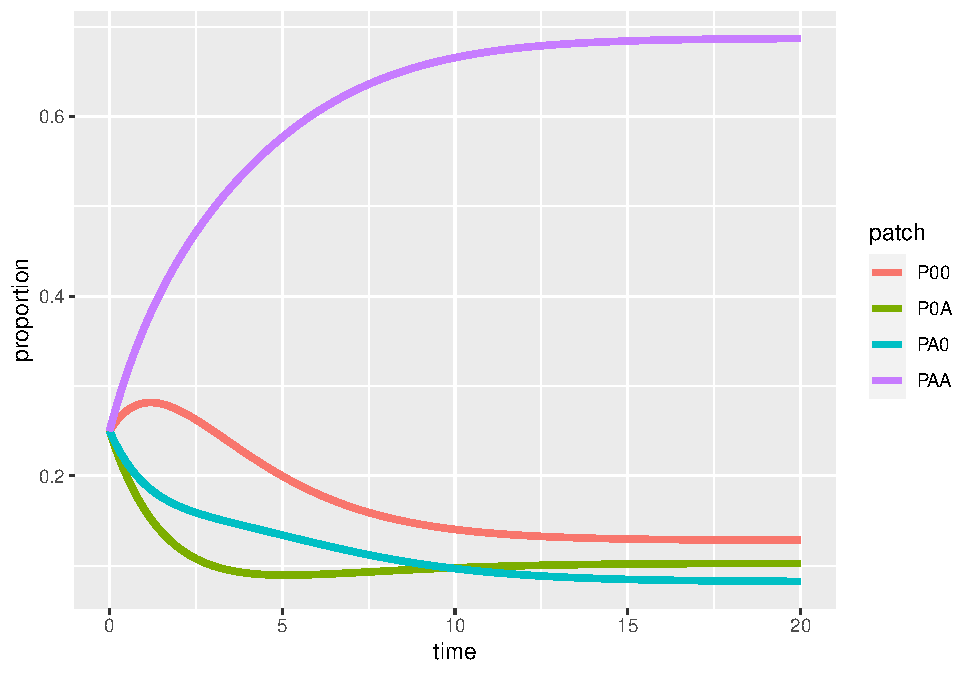
\includegraphics{bookdown-demo_files/figure-latex/unnamed-chunk-20-1.pdf}

\begin{Shaded}
\begin{Highlighting}[]
\CommentTok{### Visualization II}
\KeywordTok{plot}\NormalTok{(}\KeywordTok{range}\NormalTok{(times), }\KeywordTok{c}\NormalTok{(}\DecValTok{0}\NormalTok{,}\DecValTok{1}\NormalTok{), }\DataTypeTok{type =} \StringTok{"n"}\NormalTok{, }\DataTypeTok{xlab =} \StringTok{"time"}\NormalTok{, }\DataTypeTok{ylab =} \StringTok{"proportion"}\NormalTok{)}
\KeywordTok{lines}\NormalTok{(P00 }\OperatorTok{~}\StringTok{ }\NormalTok{time, }\DataTypeTok{data =}\NormalTok{ pop_size, }\DataTypeTok{col =} \StringTok{"tomato"}\NormalTok{)}
\KeywordTok{lines}\NormalTok{(P0A }\OperatorTok{~}\StringTok{ }\NormalTok{time, }\DataTypeTok{data =}\NormalTok{ pop_size, }\DataTypeTok{col =} \StringTok{"navy"}\NormalTok{)}
\KeywordTok{lines}\NormalTok{(PA0 }\OperatorTok{~}\StringTok{ }\NormalTok{time, }\DataTypeTok{data =}\NormalTok{ pop_size, }\DataTypeTok{col =} \StringTok{"gray"}\NormalTok{)}
\KeywordTok{lines}\NormalTok{(PAA }\OperatorTok{~}\StringTok{ }\NormalTok{time, }\DataTypeTok{data =}\NormalTok{ pop_size, }\DataTypeTok{col =} \StringTok{"orange"}\NormalTok{)}
\KeywordTok{legend}\NormalTok{(}\StringTok{"topleft"}\NormalTok{, }\DataTypeTok{legend =} \KeywordTok{c}\NormalTok{(}\StringTok{"P00"}\NormalTok{, }\StringTok{"P0A"}\NormalTok{, }\StringTok{"PA0"}\NormalTok{, }\StringTok{"PAA"}\NormalTok{), }\DataTypeTok{col =} \KeywordTok{c}\NormalTok{(}\StringTok{"tomato"}\NormalTok{, }\StringTok{"navy"}\NormalTok{, }\StringTok{"gray"}\NormalTok{, }\StringTok{"orange"}\NormalTok{), }\DataTypeTok{lty =} \DecValTok{1}\NormalTok{)}
\end{Highlighting}
\end{Shaded}

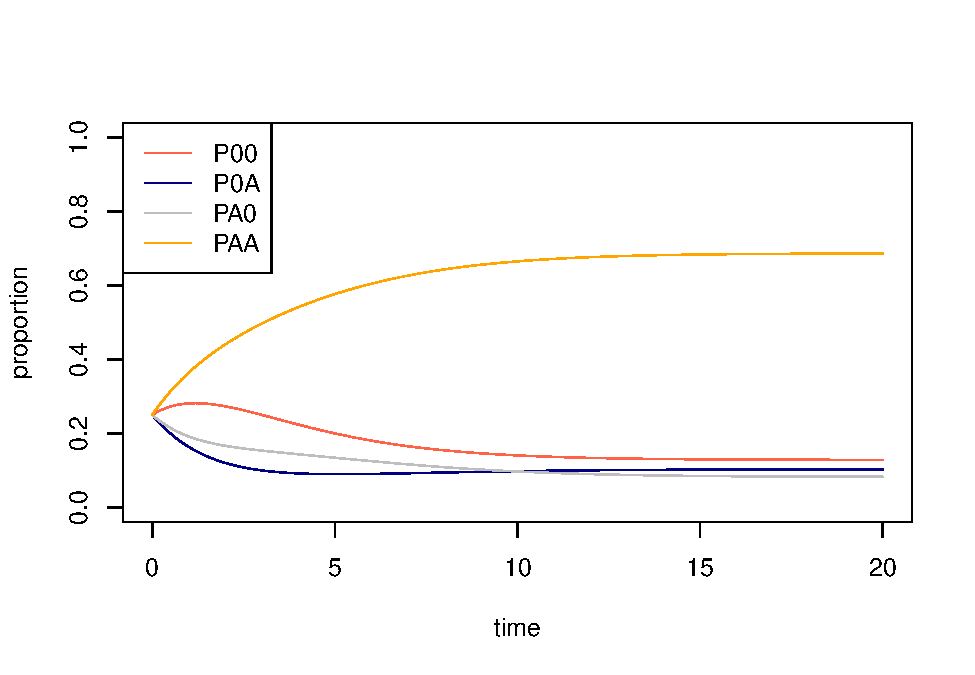
\includegraphics{bookdown-demo_files/figure-latex/unnamed-chunk-20-2.pdf}

\hypertarget{week-7---lotka-volterra-competition-model---population-dynamics}{%
\chapter*{Week 7 - Lotka-Volterra competition model - Population dynamics}\label{week-7---lotka-volterra-competition-model---population-dynamics}}
\addcontentsline{toc}{chapter}{Week 7 - Lotka-Volterra competition model - Population dynamics}

In this lab, we are going to analyze the two-species Lotka-Volterra competition model numerically and visualize the population dynamics under different parameter settings.

\begin{Shaded}
\begin{Highlighting}[]
\KeywordTok{library}\NormalTok{(ggplot2)}
\KeywordTok{library}\NormalTok{(tidyverse)}
\KeywordTok{library}\NormalTok{(deSolve)}

\NormalTok{LV_model <-}\StringTok{ }\ControlFlowTok{function}\NormalTok{(}\DataTypeTok{r1 =} \FloatTok{1.4}\NormalTok{, }\DataTypeTok{r2 =} \FloatTok{1.2}\NormalTok{, }\DataTypeTok{a11 =} \DecValTok{1}\OperatorTok{/}\DecValTok{200}\NormalTok{, }\DataTypeTok{a21 =} \DecValTok{1}\OperatorTok{/}\DecValTok{400}\NormalTok{, }\DataTypeTok{a22 =} \DecValTok{1}\OperatorTok{/}\DecValTok{200}\NormalTok{, }\DataTypeTok{a12 =} \DecValTok{1}\OperatorTok{/}\DecValTok{300}\NormalTok{, }\DataTypeTok{N1_0 =} \DecValTok{10}\NormalTok{, }\DataTypeTok{N2_0 =} \DecValTok{10}\NormalTok{) \{}

  \CommentTok{### Model specification}
\NormalTok{  LV <-}\StringTok{ }\ControlFlowTok{function}\NormalTok{(times, state, parms) \{}
    \KeywordTok{with}\NormalTok{(}\KeywordTok{as.list}\NormalTok{(}\KeywordTok{c}\NormalTok{(state, parms)), \{}
\NormalTok{      dN1_dt =}\StringTok{ }\NormalTok{N1 }\OperatorTok{*}\StringTok{ }\NormalTok{(r1 }\OperatorTok{-}\StringTok{ }\NormalTok{a11}\OperatorTok{*}\NormalTok{N1 }\OperatorTok{-}\StringTok{ }\NormalTok{a12}\OperatorTok{*}\NormalTok{N2)}
\NormalTok{      dN2_dt =}\StringTok{ }\NormalTok{N2 }\OperatorTok{*}\StringTok{ }\NormalTok{(r2 }\OperatorTok{-}\StringTok{ }\NormalTok{a22}\OperatorTok{*}\NormalTok{N2 }\OperatorTok{-}\StringTok{ }\NormalTok{a21}\OperatorTok{*}\NormalTok{N1)}
      \KeywordTok{return}\NormalTok{(}\KeywordTok{list}\NormalTok{(}\KeywordTok{c}\NormalTok{(dN1_dt, dN2_dt)))}
\NormalTok{    \})}
\NormalTok{  \}}

  \CommentTok{### Model parameters}
\NormalTok{  times <-}\StringTok{ }\KeywordTok{seq}\NormalTok{(}\DecValTok{0}\NormalTok{, }\DecValTok{100}\NormalTok{, }\DataTypeTok{by =} \FloatTok{0.1}\NormalTok{)}
\NormalTok{  state <-}\StringTok{ }\KeywordTok{c}\NormalTok{(}\DataTypeTok{N1 =}\NormalTok{ N1_}\DecValTok{0}\NormalTok{, }\DataTypeTok{N2 =}\NormalTok{ N2_}\DecValTok{0}\NormalTok{)}
\NormalTok{  parms <-}\StringTok{ }\KeywordTok{c}\NormalTok{(}\DataTypeTok{r1 =}\NormalTok{ r1, }\DataTypeTok{r2 =}\NormalTok{ r2, }\DataTypeTok{a11 =}\NormalTok{ a11, }\DataTypeTok{a21 =}\NormalTok{ a21, }\DataTypeTok{a22 =}\NormalTok{ a22, }\DataTypeTok{a12 =}\NormalTok{ a12)}

  \CommentTok{### Model application}
\NormalTok{  pop_size <-}\StringTok{ }\KeywordTok{ode}\NormalTok{(}\DataTypeTok{func =}\NormalTok{ LV, }\DataTypeTok{times =}\NormalTok{ times, }\DataTypeTok{y =}\NormalTok{ state, }\DataTypeTok{parms =}\NormalTok{ parms)}

  \CommentTok{### Visualize the population dynamics}
\NormalTok{  pop_size }\OperatorTok
\StringTok{    }\KeywordTok{as.data.frame}\NormalTok{() }\OperatorTok
\StringTok{    }\KeywordTok{gather}\NormalTok{(}\DataTypeTok{key =} \StringTok{"Species"}\NormalTok{, }\DataTypeTok{value =} \StringTok{"pop_size"}\NormalTok{, }\OperatorTok{-}\NormalTok{time) }\OperatorTok
\StringTok{    }\KeywordTok{ggplot}\NormalTok{(}\KeywordTok{aes}\NormalTok{(}\DataTypeTok{x =}\NormalTok{ time, }\DataTypeTok{y =}\NormalTok{ pop_size, }\DataTypeTok{color =}\NormalTok{ Species)) }\OperatorTok{+}
\StringTok{    }\KeywordTok{geom_line}\NormalTok{(}\DataTypeTok{size =} \FloatTok{1.5}\NormalTok{)}

\NormalTok{\}}

  \CommentTok{### Different parameter settings}
  \CommentTok{## N1_0 = 200 and N2_0 = 5}
  \KeywordTok{LV_model}\NormalTok{(}\DataTypeTok{r1 =} \FloatTok{1.2}\NormalTok{, }\DataTypeTok{r2 =} \FloatTok{1.2}\NormalTok{, }\DataTypeTok{a11 =} \DecValTok{1}\OperatorTok{/}\DecValTok{200}\NormalTok{, }\DataTypeTok{a21 =} \DecValTok{1}\OperatorTok{/}\DecValTok{100}\NormalTok{, }\DataTypeTok{a22 =} \DecValTok{1}\OperatorTok{/}\DecValTok{100}\NormalTok{, }\DataTypeTok{a12 =} \DecValTok{1}\OperatorTok{/}\DecValTok{200}\NormalTok{, }\DataTypeTok{N1_0 =} \DecValTok{200}\NormalTok{, }\DataTypeTok{N2_0 =} \DecValTok{5}\NormalTok{)  }\CommentTok{# N1 wins}
\end{Highlighting}
\end{Shaded}

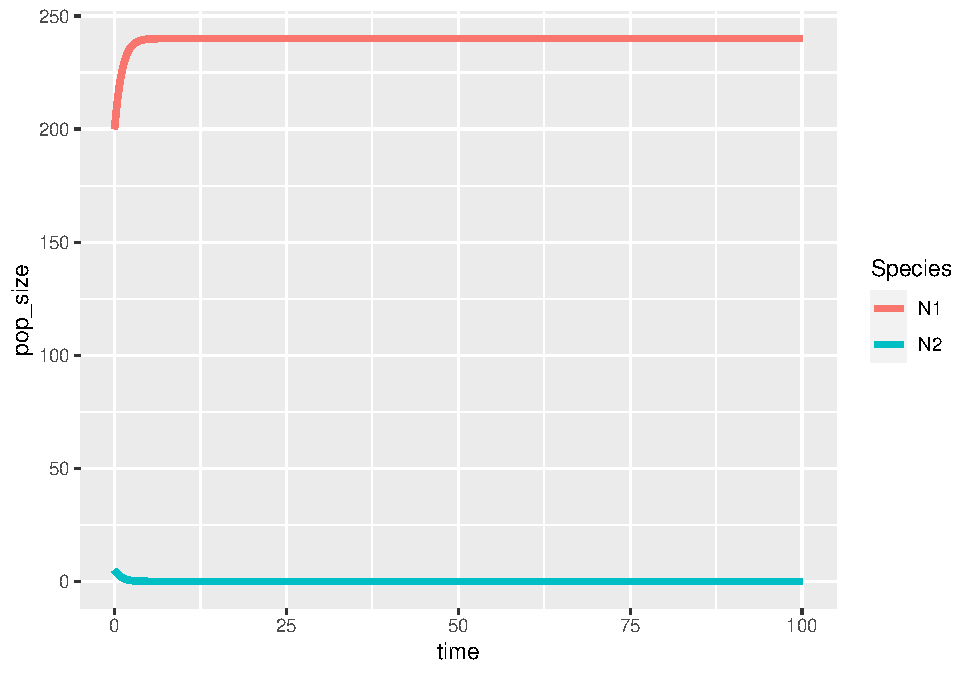
\includegraphics{bookdown-demo_files/figure-latex/unnamed-chunk-21-1.pdf}

\begin{Shaded}
\begin{Highlighting}[]
  \CommentTok{## N1_0 = 5 and N2_0 = 200}
  \KeywordTok{LV_model}\NormalTok{(}\DataTypeTok{r1 =} \FloatTok{1.2}\NormalTok{, }\DataTypeTok{r2 =} \FloatTok{1.2}\NormalTok{, }\DataTypeTok{a11 =} \DecValTok{1}\OperatorTok{/}\DecValTok{200}\NormalTok{, }\DataTypeTok{a21 =} \DecValTok{1}\OperatorTok{/}\DecValTok{100}\NormalTok{, }\DataTypeTok{a22 =} \DecValTok{1}\OperatorTok{/}\DecValTok{100}\NormalTok{, }\DataTypeTok{a12 =} \DecValTok{1}\OperatorTok{/}\DecValTok{200}\NormalTok{, }\DataTypeTok{N1_0 =} \DecValTok{10}\NormalTok{, }\DataTypeTok{N2_0 =} \DecValTok{200}\NormalTok{)  }\CommentTok{# N1 wins}
\end{Highlighting}
\end{Shaded}

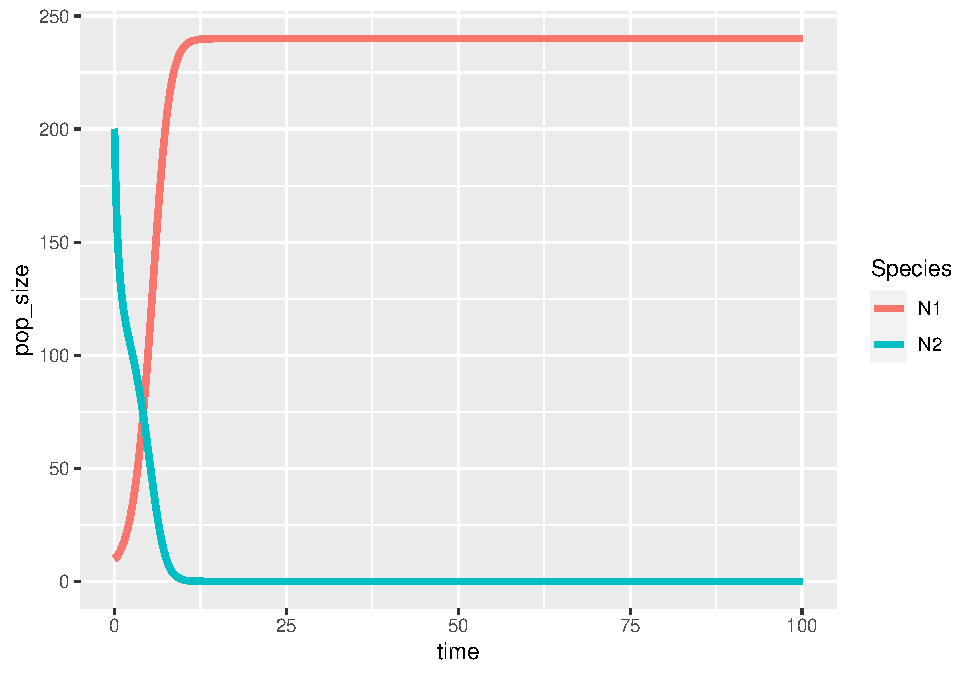
\includegraphics{bookdown-demo_files/figure-latex/unnamed-chunk-21-2.pdf}

\begin{Shaded}
\begin{Highlighting}[]
  \CommentTok{## N1_0 = 200 and N2_0 = 5}
  \KeywordTok{LV_model}\NormalTok{(}\DataTypeTok{r1 =} \FloatTok{1.2}\NormalTok{, }\DataTypeTok{r2 =} \FloatTok{1.2}\NormalTok{, }\DataTypeTok{a11 =} \DecValTok{1}\OperatorTok{/}\DecValTok{100}\NormalTok{, }\DataTypeTok{a21 =} \DecValTok{1}\OperatorTok{/}\DecValTok{200}\NormalTok{, }\DataTypeTok{a22 =} \DecValTok{1}\OperatorTok{/}\DecValTok{200}\NormalTok{, }\DataTypeTok{a12 =} \DecValTok{1}\OperatorTok{/}\DecValTok{100}\NormalTok{, }\DataTypeTok{N1_0 =} \DecValTok{200}\NormalTok{, }\DataTypeTok{N2_0 =} \DecValTok{5}\NormalTok{)  }\CommentTok{# N2 wins}
\end{Highlighting}
\end{Shaded}

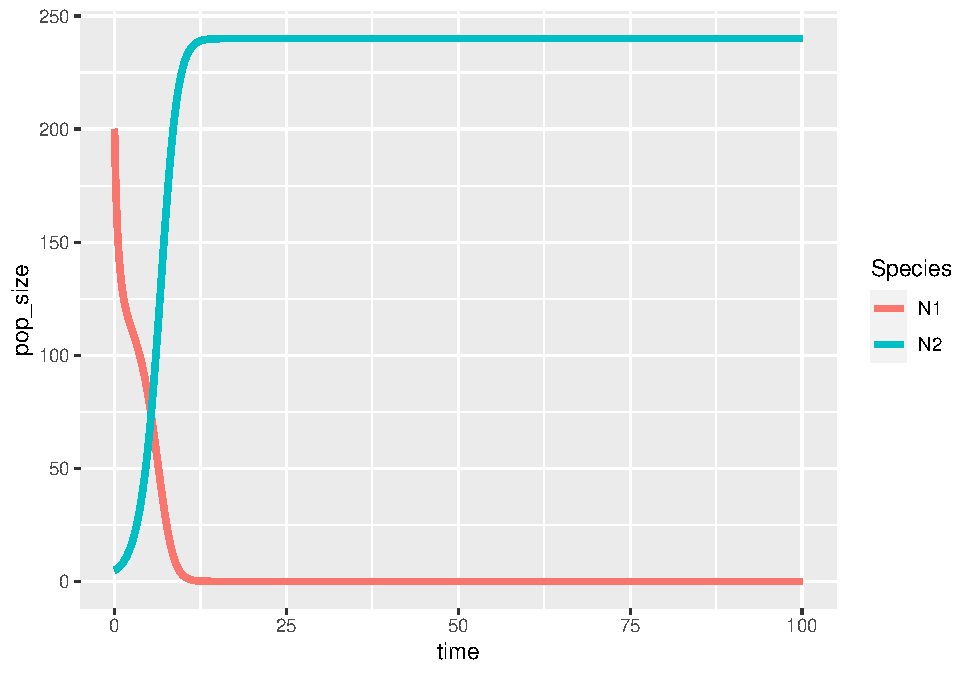
\includegraphics{bookdown-demo_files/figure-latex/unnamed-chunk-21-3.pdf}

\begin{Shaded}
\begin{Highlighting}[]
  \CommentTok{## N1_0 = 5 and N2_0 = 200}
  \KeywordTok{LV_model}\NormalTok{(}\DataTypeTok{r1 =} \FloatTok{1.2}\NormalTok{, }\DataTypeTok{r2 =} \FloatTok{1.2}\NormalTok{, }\DataTypeTok{a11 =} \DecValTok{1}\OperatorTok{/}\DecValTok{100}\NormalTok{, }\DataTypeTok{a21 =} \DecValTok{1}\OperatorTok{/}\DecValTok{200}\NormalTok{, }\DataTypeTok{a22 =} \DecValTok{1}\OperatorTok{/}\DecValTok{200}\NormalTok{, }\DataTypeTok{a12 =} \DecValTok{1}\OperatorTok{/}\DecValTok{100}\NormalTok{, }\DataTypeTok{N1_0 =} \DecValTok{5}\NormalTok{, }\DataTypeTok{N2_0 =} \DecValTok{200}\NormalTok{)  }\CommentTok{# N2 wins}
\end{Highlighting}
\end{Shaded}

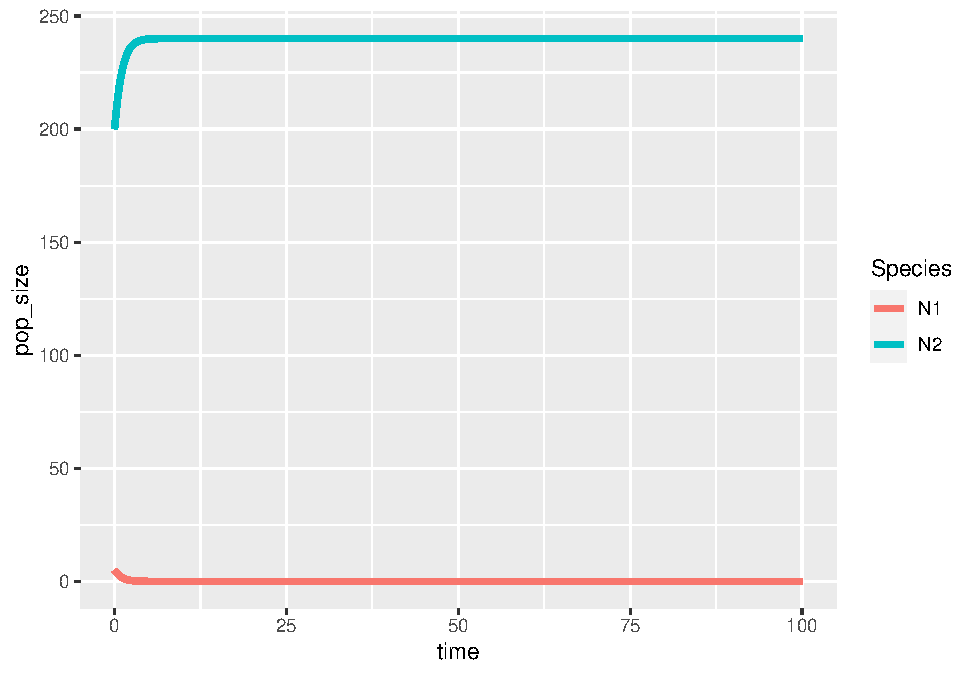
\includegraphics{bookdown-demo_files/figure-latex/unnamed-chunk-21-4.pdf}

\begin{Shaded}
\begin{Highlighting}[]
  \CommentTok{## N1_0 = 200 and N2_0 = 5}
  \KeywordTok{LV_model}\NormalTok{(}\DataTypeTok{r1 =} \FloatTok{1.2}\NormalTok{, }\DataTypeTok{r2 =} \FloatTok{1.2}\NormalTok{, }\DataTypeTok{a11 =} \DecValTok{1}\OperatorTok{/}\DecValTok{100}\NormalTok{, }\DataTypeTok{a21 =} \DecValTok{1}\OperatorTok{/}\DecValTok{200}\NormalTok{, }\DataTypeTok{a22 =} \DecValTok{1}\OperatorTok{/}\DecValTok{100}\NormalTok{, }\DataTypeTok{a12 =} \DecValTok{1}\OperatorTok{/}\DecValTok{300}\NormalTok{, }\DataTypeTok{N1_0 =} \DecValTok{200}\NormalTok{, }\DataTypeTok{N2_0 =} \DecValTok{5}\NormalTok{)  }\CommentTok{# stable coexistence}
\end{Highlighting}
\end{Shaded}

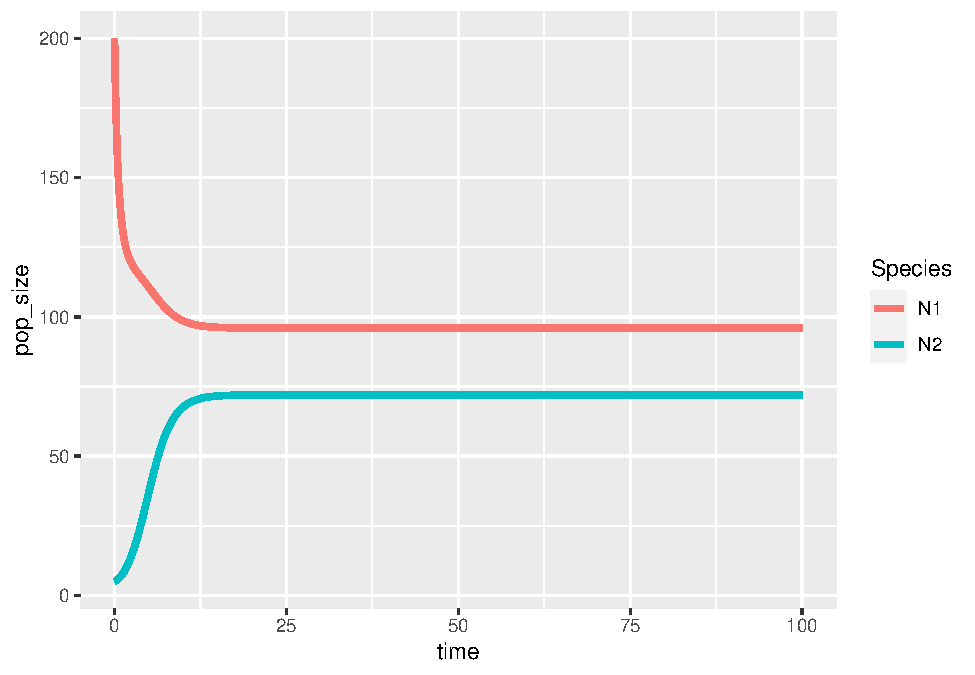
\includegraphics{bookdown-demo_files/figure-latex/unnamed-chunk-21-5.pdf}

\begin{Shaded}
\begin{Highlighting}[]
  \CommentTok{## N1_0 = 5 and N2_0 = 200}
  \KeywordTok{LV_model}\NormalTok{(}\DataTypeTok{r1 =} \FloatTok{1.2}\NormalTok{, }\DataTypeTok{r2 =} \FloatTok{1.2}\NormalTok{, }\DataTypeTok{a11 =} \DecValTok{1}\OperatorTok{/}\DecValTok{100}\NormalTok{, }\DataTypeTok{a21 =} \DecValTok{1}\OperatorTok{/}\DecValTok{200}\NormalTok{, }\DataTypeTok{a22 =} \DecValTok{1}\OperatorTok{/}\DecValTok{100}\NormalTok{, }\DataTypeTok{a12 =} \DecValTok{1}\OperatorTok{/}\DecValTok{300}\NormalTok{, }\DataTypeTok{N1_0 =} \DecValTok{5}\NormalTok{, }\DataTypeTok{N2_0 =} \DecValTok{200}\NormalTok{)  }\CommentTok{# stable coexistence}
\end{Highlighting}
\end{Shaded}

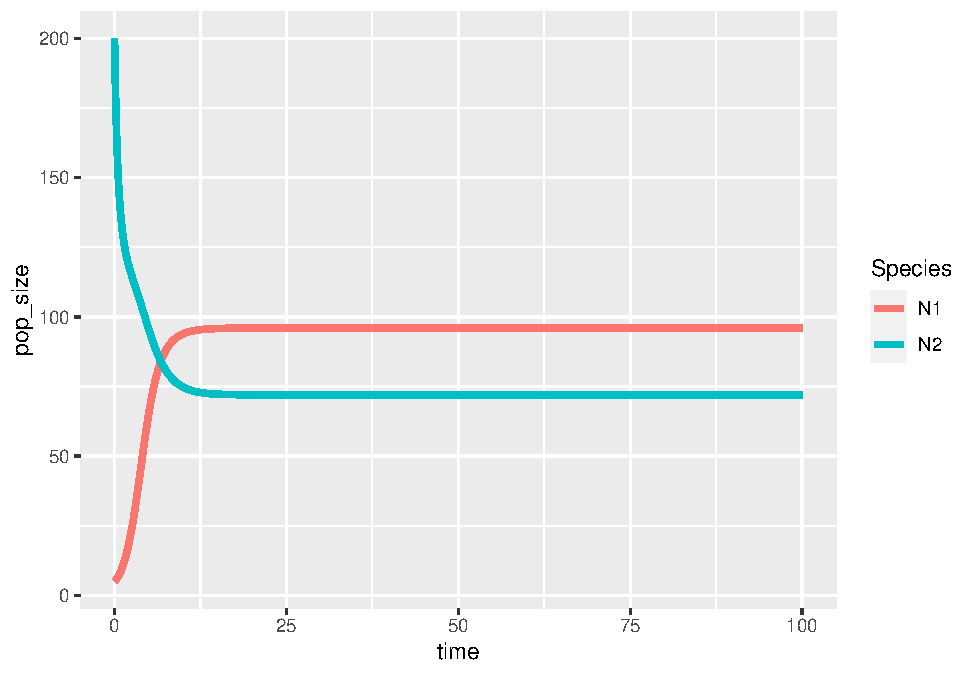
\includegraphics{bookdown-demo_files/figure-latex/unnamed-chunk-21-6.pdf}

\begin{Shaded}
\begin{Highlighting}[]
  \CommentTok{## N1_0 = 200 and N2_0 = 150}
  \KeywordTok{LV_model}\NormalTok{(}\DataTypeTok{r1 =} \FloatTok{1.2}\NormalTok{, }\DataTypeTok{r2 =} \FloatTok{1.2}\NormalTok{, }\DataTypeTok{a11 =} \DecValTok{1}\OperatorTok{/}\DecValTok{200}\NormalTok{, }\DataTypeTok{a21 =} \DecValTok{1}\OperatorTok{/}\DecValTok{100}\NormalTok{, }\DataTypeTok{a22 =} \DecValTok{1}\OperatorTok{/}\DecValTok{200}\NormalTok{, }\DataTypeTok{a12 =} \DecValTok{1}\OperatorTok{/}\DecValTok{100}\NormalTok{, }\DataTypeTok{N1_0 =} \DecValTok{200}\NormalTok{, }\DataTypeTok{N2_0 =} \DecValTok{150}\NormalTok{)  }\CommentTok{# priority effect (N1 wins)}
\end{Highlighting}
\end{Shaded}

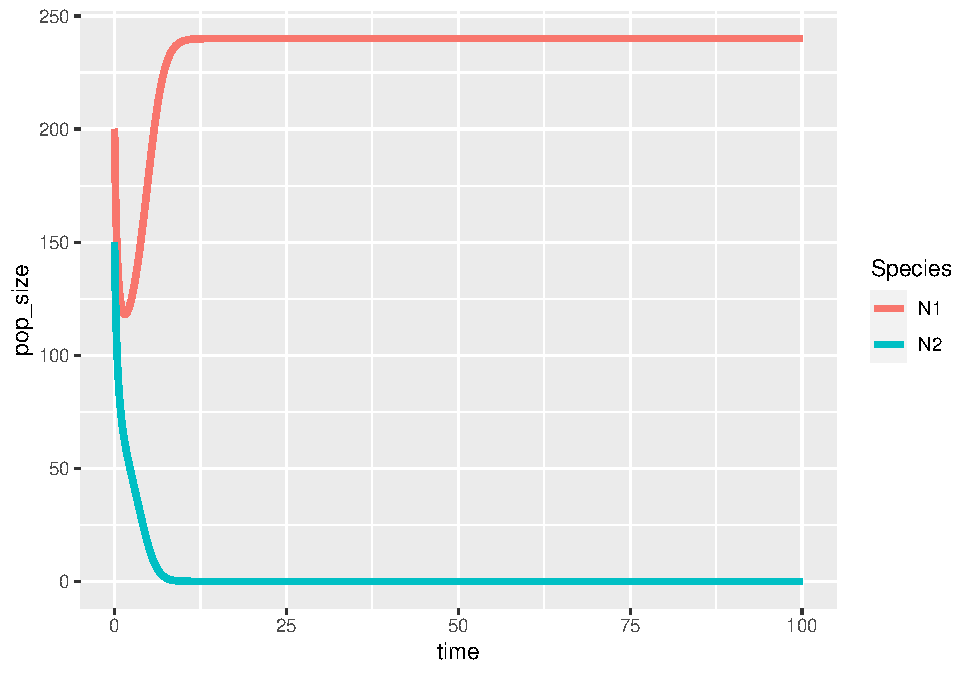
\includegraphics{bookdown-demo_files/figure-latex/unnamed-chunk-21-7.pdf}

\begin{Shaded}
\begin{Highlighting}[]
  \CommentTok{## N1_0 = 150 and N2_0 = 200}
  \KeywordTok{LV_model}\NormalTok{(}\DataTypeTok{r1 =} \FloatTok{1.2}\NormalTok{, }\DataTypeTok{r2 =} \FloatTok{1.2}\NormalTok{, }\DataTypeTok{a11 =} \DecValTok{1}\OperatorTok{/}\DecValTok{200}\NormalTok{, }\DataTypeTok{a21 =} \DecValTok{1}\OperatorTok{/}\DecValTok{100}\NormalTok{, }\DataTypeTok{a22 =} \DecValTok{1}\OperatorTok{/}\DecValTok{200}\NormalTok{, }\DataTypeTok{a12 =} \DecValTok{1}\OperatorTok{/}\DecValTok{100}\NormalTok{, }\DataTypeTok{N1_0 =} \DecValTok{150}\NormalTok{, }\DataTypeTok{N2_0 =} \DecValTok{200}\NormalTok{)  }\CommentTok{# priority effect (N2 wins)}
\end{Highlighting}
\end{Shaded}

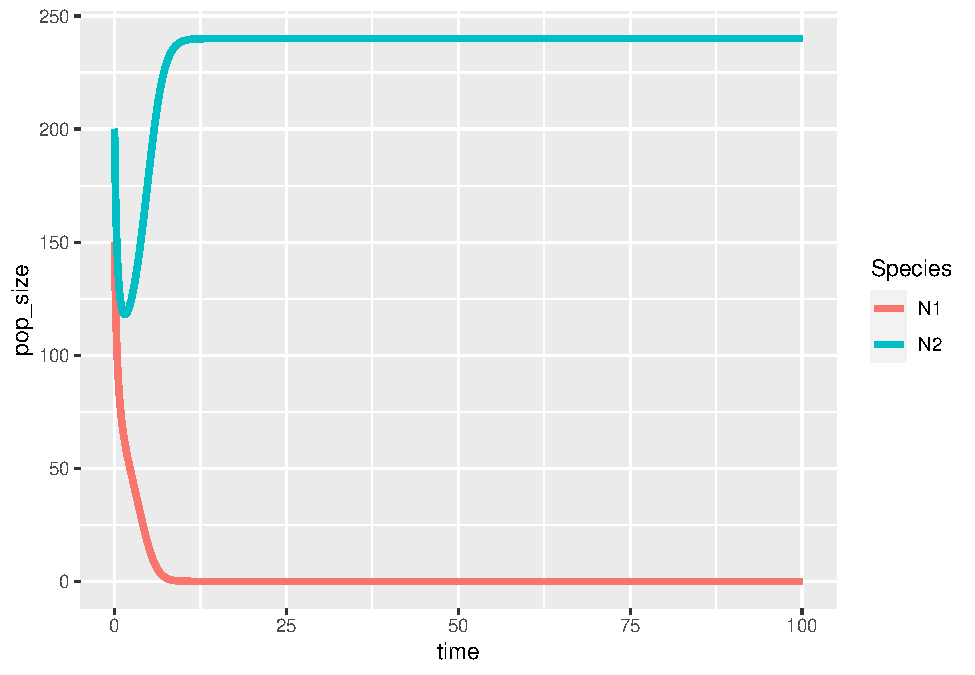
\includegraphics{bookdown-demo_files/figure-latex/unnamed-chunk-21-8.pdf}

\begin{Shaded}
\begin{Highlighting}[]
\CommentTok{#### phase diagram}
\NormalTok{phase_plane <-}\StringTok{ }\ControlFlowTok{function}\NormalTok{(r1, r2, a11, a21, a22, a12, title, t)\{}
    \CommentTok{### Vectors}
\NormalTok{  LV <-}\StringTok{ }\ControlFlowTok{function}\NormalTok{(times, state, parms) \{}
    \KeywordTok{with}\NormalTok{(}\KeywordTok{as.list}\NormalTok{(}\KeywordTok{c}\NormalTok{(state, parms)), \{}
\NormalTok{      dN1_dt =}\StringTok{ }\NormalTok{N1 }\OperatorTok{*}\StringTok{ }\NormalTok{(r1 }\OperatorTok{-}\StringTok{ }\NormalTok{a11}\OperatorTok{*}\NormalTok{N1 }\OperatorTok{-}\StringTok{ }\NormalTok{a12}\OperatorTok{*}\NormalTok{N2)}
\NormalTok{      dN2_dt =}\StringTok{ }\NormalTok{N2 }\OperatorTok{*}\StringTok{ }\NormalTok{(r2 }\OperatorTok{-}\StringTok{ }\NormalTok{a22}\OperatorTok{*}\NormalTok{N2 }\OperatorTok{-}\StringTok{ }\NormalTok{a21}\OperatorTok{*}\NormalTok{N1)}
      \KeywordTok{return}\NormalTok{(}\KeywordTok{list}\NormalTok{(}\KeywordTok{c}\NormalTok{(dN1_dt, dN2_dt)))}
\NormalTok{    \})}
\NormalTok{  \}}

\NormalTok{  times <-}\StringTok{ }\KeywordTok{c}\NormalTok{(}\DecValTok{0}\NormalTok{, t)}
\NormalTok{  parms <-}\StringTok{ }\KeywordTok{c}\NormalTok{(}\DataTypeTok{r1 =}\NormalTok{ r1, }\DataTypeTok{r2 =}\NormalTok{ r2, }\DataTypeTok{a11 =}\NormalTok{ a11, }\DataTypeTok{a21 =}\NormalTok{ a21, }\DataTypeTok{a22 =}\NormalTok{ a22, }\DataTypeTok{a12 =}\NormalTok{ a12)}

\NormalTok{  x_inter<-}\StringTok{ }\KeywordTok{max}\NormalTok{(}\KeywordTok{c}\NormalTok{(r1}\OperatorTok{/}\NormalTok{a11, r2}\OperatorTok{/}\NormalTok{a21))}
\NormalTok{  y_inter <-}\StringTok{ }\KeywordTok{max}\NormalTok{(}\KeywordTok{c}\NormalTok{(r2}\OperatorTok{/}\NormalTok{a22, r1}\OperatorTok{/}\NormalTok{a12))}

  \CommentTok{# create position of arrows}
\NormalTok{  vector_grid <-}\StringTok{ }\KeywordTok{expand.grid}\NormalTok{(}\KeywordTok{seq}\NormalTok{(}\DecValTok{5}\NormalTok{, x_inter, }\DataTypeTok{length.out =} \DecValTok{10}\NormalTok{),}
                             \KeywordTok{seq}\NormalTok{(}\DecValTok{5}\NormalTok{, y_inter, }\DataTypeTok{length.out =} \DecValTok{10}\NormalTok{))}

\NormalTok{  vector_data <-}\StringTok{ }\NormalTok{vector_grid }\OperatorTok
\StringTok{    }\KeywordTok{pmap}\NormalTok{(., }\ControlFlowTok{function}\NormalTok{(Var1, Var2)\{}
\NormalTok{      state <-}\StringTok{ }\KeywordTok{c}\NormalTok{(}\DataTypeTok{N1 =}\NormalTok{ Var1, }\DataTypeTok{N2 =}\NormalTok{ Var2)}
\NormalTok{      pop_size <-}\StringTok{ }\KeywordTok{ode}\NormalTok{(}\DataTypeTok{func =}\NormalTok{ LV, }\DataTypeTok{times =}\NormalTok{ times, }\DataTypeTok{y =}\NormalTok{ state, }\DataTypeTok{parms =}\NormalTok{ parms)}
\NormalTok{      pop_size[}\DecValTok{2}\NormalTok{, }\DecValTok{2}\OperatorTok{:}\DecValTok{3}\NormalTok{]}
\NormalTok{    \}) }\OperatorTok
\StringTok{    }\KeywordTok{bind_rows}\NormalTok{() }\OperatorTok
\StringTok{    }\KeywordTok{rename}\NormalTok{(}\DataTypeTok{xend =}\NormalTok{ N1, }\DataTypeTok{yend =}\NormalTok{ N2) }\OperatorTok
\StringTok{    }\KeywordTok{bind_cols}\NormalTok{(vector_grid) }\OperatorTok
\StringTok{    }\KeywordTok{rename}\NormalTok{(}\DataTypeTok{x =}\NormalTok{ Var1, }\DataTypeTok{y =}\NormalTok{ Var2)}

    \CommentTok{### Phase plane}
    \KeywordTok{ggplot}\NormalTok{() }\OperatorTok{+}
\StringTok{      }\KeywordTok{geom_abline}\NormalTok{(}\DataTypeTok{slope =} \OperatorTok{-}\NormalTok{a11}\OperatorTok{/}\NormalTok{a12, }\DataTypeTok{intercept =}\NormalTok{ r1}\OperatorTok{/}\NormalTok{a12, }\DataTypeTok{color =} \StringTok{"#E41A1C"}\NormalTok{, }\DataTypeTok{size =} \FloatTok{1.5}\NormalTok{) }\OperatorTok{+}
\StringTok{      }\KeywordTok{geom_abline}\NormalTok{(}\DataTypeTok{slope =} \OperatorTok{-}\NormalTok{a21}\OperatorTok{/}\NormalTok{a22, }\DataTypeTok{intercept =}\NormalTok{ r2}\OperatorTok{/}\NormalTok{a22, }\DataTypeTok{color =} \StringTok{"#377EB8"}\NormalTok{, }\DataTypeTok{size =} \FloatTok{1.5}\NormalTok{) }\OperatorTok{+}
\StringTok{      }\KeywordTok{geom_segment}\NormalTok{(}\DataTypeTok{data =}\NormalTok{ vector_data,}
                   \KeywordTok{aes}\NormalTok{(}\DataTypeTok{x =}\NormalTok{ x, }\DataTypeTok{y =}\NormalTok{ y, }\DataTypeTok{xend =}\NormalTok{ xend, }\DataTypeTok{yend =}\NormalTok{ yend),}
                   \DataTypeTok{arrow =} \KeywordTok{arrow}\NormalTok{(}\DataTypeTok{length =} \KeywordTok{unit}\NormalTok{(}\FloatTok{0.1}\NormalTok{, }\StringTok{"cm"}\NormalTok{))) }\OperatorTok{+}\StringTok{    }
\StringTok{      }\KeywordTok{scale_x_continuous}\NormalTok{(}\DataTypeTok{name =} \StringTok{"N1"}\NormalTok{, }\DataTypeTok{limits =} \KeywordTok{c}\NormalTok{(}\DecValTok{0}\NormalTok{, x_inter), }\DataTypeTok{expand =} \KeywordTok{c}\NormalTok{(}\DecValTok{0}\NormalTok{, }\DecValTok{0}\NormalTok{)) }\OperatorTok{+}
\StringTok{      }\KeywordTok{scale_y_continuous}\NormalTok{(}\DataTypeTok{name =} \StringTok{"N2"}\NormalTok{, }\DataTypeTok{limits =} \KeywordTok{c}\NormalTok{(}\DecValTok{0}\NormalTok{, y_inter), }\DataTypeTok{expand =} \KeywordTok{c}\NormalTok{(}\DecValTok{0}\NormalTok{, }\DecValTok{0}\NormalTok{)) }\OperatorTok{+}
\StringTok{      }\KeywordTok{theme_bw}\NormalTok{(}\DataTypeTok{base_size =} \DecValTok{13}\NormalTok{) }\OperatorTok{+}
\StringTok{      }\KeywordTok{theme}\NormalTok{(}\DataTypeTok{panel.grid =} \KeywordTok{element_blank}\NormalTok{(),}
            \DataTypeTok{plot.title =} \KeywordTok{element_text}\NormalTok{(}\DataTypeTok{hjust =} \FloatTok{0.5}\NormalTok{)) }\OperatorTok{+}
\StringTok{      }\KeywordTok{labs}\NormalTok{(}\DataTypeTok{title =}\NormalTok{ title)}
\NormalTok{  \}}

  \KeywordTok{phase_plane}\NormalTok{(}\DataTypeTok{r1 =} \FloatTok{1.2}\NormalTok{, }\DataTypeTok{r2 =} \FloatTok{1.2}\NormalTok{, }\DataTypeTok{a11 =} \DecValTok{1}\OperatorTok{/}\DecValTok{100}\NormalTok{, }\DataTypeTok{a21 =} \DecValTok{1}\OperatorTok{/}\DecValTok{200}\NormalTok{, }\DataTypeTok{a22 =} \DecValTok{1}\OperatorTok{/}\DecValTok{100}\NormalTok{, }\DataTypeTok{a12 =} \DecValTok{1}\OperatorTok{/}\DecValTok{300}\NormalTok{, }\DataTypeTok{t =} \FloatTok{0.3}\NormalTok{, }\DataTypeTok{title =} \StringTok{"Stable coexistence"}\NormalTok{)}
\end{Highlighting}
\end{Shaded}

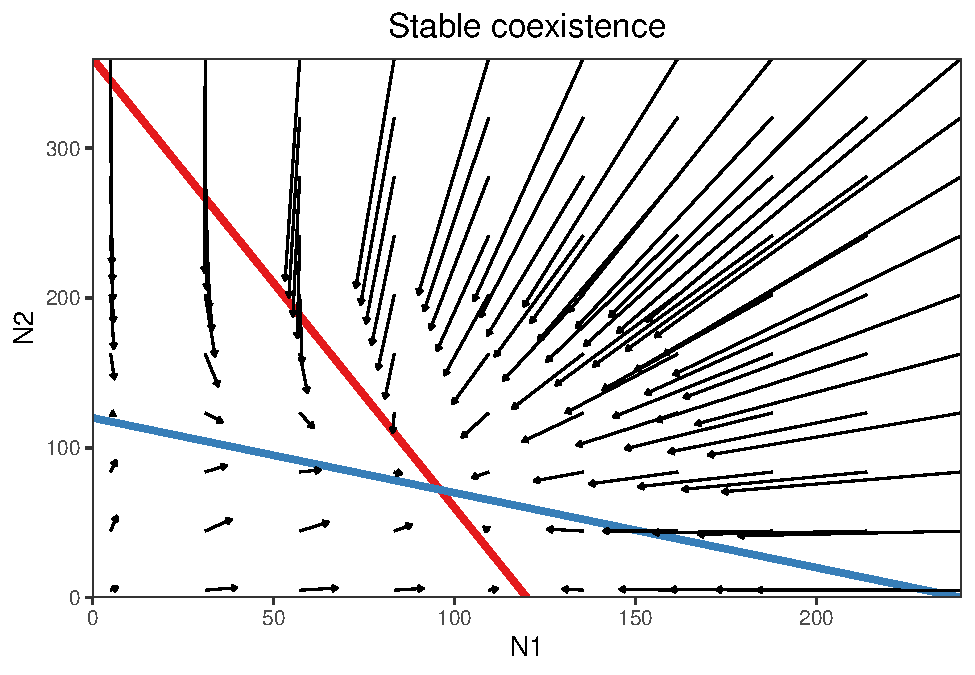
\includegraphics{bookdown-demo_files/figure-latex/unnamed-chunk-22-1.pdf}

\begin{Shaded}
\begin{Highlighting}[]
  \KeywordTok{phase_plane}\NormalTok{(}\DataTypeTok{r1 =} \FloatTok{1.2}\NormalTok{, }\DataTypeTok{r2 =} \FloatTok{1.2}\NormalTok{, }\DataTypeTok{a11 =} \DecValTok{1}\OperatorTok{/}\DecValTok{200}\NormalTok{, }\DataTypeTok{a21 =} \DecValTok{1}\OperatorTok{/}\DecValTok{100}\NormalTok{, }\DataTypeTok{a22 =} \DecValTok{1}\OperatorTok{/}\DecValTok{200}\NormalTok{, }\DataTypeTok{a12 =} \DecValTok{1}\OperatorTok{/}\DecValTok{100}\NormalTok{, }\DataTypeTok{t =} \FloatTok{0.3}\NormalTok{, }\DataTypeTok{title =} \StringTok{"Unstable coexistence (saddle)"}\NormalTok{)}
\end{Highlighting}
\end{Shaded}

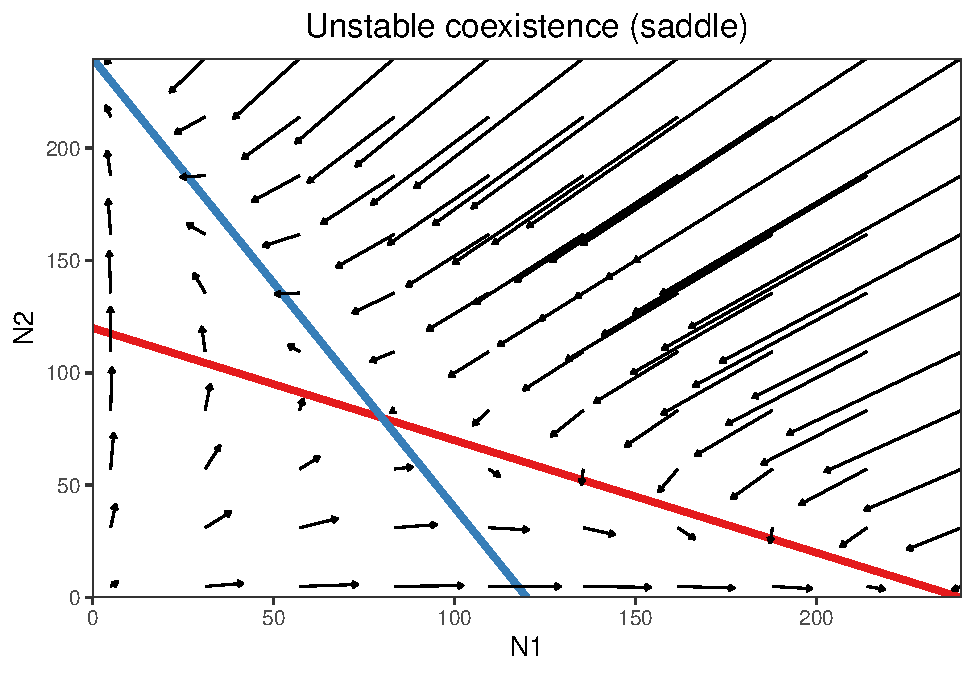
\includegraphics{bookdown-demo_files/figure-latex/unnamed-chunk-22-2.pdf}

\hypertarget{week-8---midterm}{%
\chapter*{Week 8 - Midterm}\label{week-8---midterm}}
\addcontentsline{toc}{chapter}{Week 8 - Midterm}

\hypertarget{week-9---lotka-volterra-competition-model---visualization-of-dynamics-with-complex-eigenvalues}{%
\chapter*{Week 9 - Lotka-Volterra competition model - Visualization of dynamics with complex eigenvalues}\label{week-9---lotka-volterra-competition-model---visualization-of-dynamics-with-complex-eigenvalues}}
\addcontentsline{toc}{chapter}{Week 9 - Lotka-Volterra competition model - Visualization of dynamics with complex eigenvalues}

Consider a linear system
\[
\dfrac{d \vec{\pmb\varepsilon}}{d t} = \mathcal{J}\vec{\pmb\varepsilon}
\]
where \(\vec{\pmb\varepsilon} = (\varepsilon_1, \varepsilon_2)^T\) and \(\mathcal{J} = \begin{pmatrix} -1 & 1\\ -2 & -1 \end{pmatrix}\).
Or, we can write the linear system by two ODEs:
\begin{align*}
  \dfrac{d \varepsilon_1}{d t} &= (-1)\times \varepsilon_1 + (1)\times\varepsilon_2\\
  \dfrac{d \varepsilon_2}{d t} &= (-2)\times \varepsilon_1 + (-1)\times\varepsilon_2\\
\end{align*}

Note that the element in the first row and second column is positive.

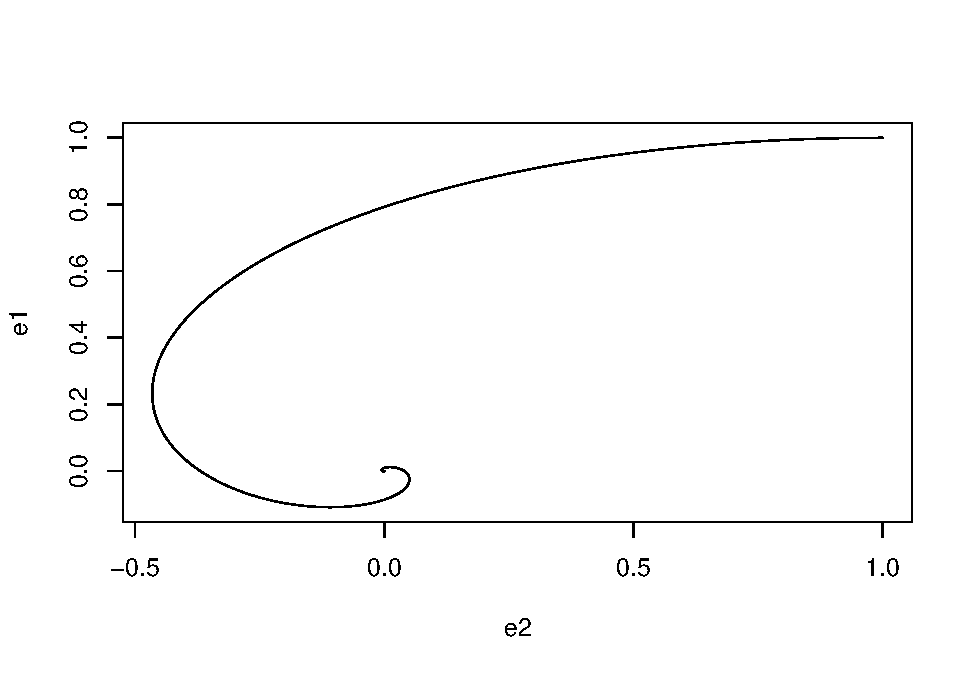
\includegraphics{bookdown-demo_files/figure-latex/unnamed-chunk-23-1.pdf}

\begin{verbatim}
##              time           e1            e2
##  [99996,]  9.9995 3.192479e-05 -6.443030e-05
##  [99997,]  9.9996 3.191516e-05 -6.443024e-05
##  [99998,]  9.9997 3.190552e-05 -6.443018e-05
##  [99999,]  9.9998 3.189589e-05 -6.443011e-05
## [100000,]  9.9999 3.188626e-05 -6.443005e-05
## [100001,] 10.0000 3.187663e-05 -6.442998e-05
\end{verbatim}

\includegraphics{W9_dynamics_error.gif}

\hypertarget{week-10---lotka-volterra-model-of-predator-prey-interactions-and-time-scale-separation}{%
\chapter*{Week 10 - Lotka-Volterra model of predator-prey interactions and time-scale separation}\label{week-10---lotka-volterra-model-of-predator-prey-interactions-and-time-scale-separation}}
\addcontentsline{toc}{chapter}{Week 10 - Lotka-Volterra model of predator-prey interactions and time-scale separation}

\textbf{Part 1: analyzing the classic Lotka-Volterra predator-prey model}

In this lab, we are going to analyze the classic Lotka-Volterra predator-prey model:

\begin{align*}
\frac {dN}{dt} &= rN-aNP\\
\frac {dP}{dt} &= eaNP-dP
\end{align*}

The non-trivial equilibrium of this system is \(E_c = (N = \frac{d}{ea}, P = \frac{r}{a})\).

We simulate the model using the following parameter set (\(N_0\) = 10, \(P_0\) = 2, \(r\) = 1.0, \(a\) = 0.1, \(e\) = 0.8, \(d\) = 0.5) and plot the population trajectories of predator and prey over time. We also show their population dynamics in the state-space diagram.

What will happen if you add a perturbation to the system (i.e., change the initial conditions)? Try out different values of \(N\) and \(P\) and visualize the differences in the state-space diagram by yourselve.

\begin{Shaded}
\begin{Highlighting}[]
\KeywordTok{library}\NormalTok{(deSolve)}
\CommentTok{### Model specification}
\NormalTok{LV_predation_model <-}\StringTok{ }\ControlFlowTok{function}\NormalTok{(times, state, parms) \{}
  \KeywordTok{with}\NormalTok{(}\KeywordTok{as.list}\NormalTok{(}\KeywordTok{c}\NormalTok{(state, parms)), \{}
\NormalTok{    dN_dt =}\StringTok{ }\NormalTok{r}\OperatorTok{*}\NormalTok{N }\OperatorTok{-}\StringTok{ }\NormalTok{a}\OperatorTok{*}\NormalTok{N}\OperatorTok{*}\NormalTok{P}
\NormalTok{    dP_dt =}\StringTok{ }\NormalTok{e}\OperatorTok{*}\NormalTok{a}\OperatorTok{*}\NormalTok{N}\OperatorTok{*}\NormalTok{P }\OperatorTok{-}\StringTok{ }\NormalTok{d}\OperatorTok{*}\NormalTok{P}
    \KeywordTok{return}\NormalTok{(}\KeywordTok{list}\NormalTok{(}\KeywordTok{c}\NormalTok{(dN_dt, dP_dt)))}
\NormalTok{  \})}
\NormalTok{\}}

\CommentTok{### Model parameters}
\NormalTok{times <-}\StringTok{ }\KeywordTok{seq}\NormalTok{(}\DecValTok{0}\NormalTok{, }\DecValTok{100}\NormalTok{, }\DataTypeTok{by =} \FloatTok{0.01}\NormalTok{)}
\NormalTok{state <-}\StringTok{ }\KeywordTok{c}\NormalTok{(}\DataTypeTok{N =} \DecValTok{10}\NormalTok{, }\DataTypeTok{P =} \DecValTok{2}\NormalTok{)}
\NormalTok{parms <-}\StringTok{ }\KeywordTok{c}\NormalTok{(}\DataTypeTok{r =} \FloatTok{1.0}\NormalTok{, }\DataTypeTok{a =} \FloatTok{0.1}\NormalTok{, }\DataTypeTok{e =} \FloatTok{0.8}\NormalTok{, }\DataTypeTok{d =} \FloatTok{0.5}\NormalTok{)}

\CommentTok{### Model application}
\NormalTok{pop_size <-}\StringTok{ }\KeywordTok{ode}\NormalTok{(}\DataTypeTok{func =}\NormalTok{ LV_predation_model, }\DataTypeTok{times =}\NormalTok{ times, }\DataTypeTok{y =}\NormalTok{ state, }\DataTypeTok{parms =}\NormalTok{ parms)}

\CommentTok{### Visualization -- population dynamics}
\KeywordTok{plot}\NormalTok{(}\KeywordTok{c}\NormalTok{(}\DecValTok{0}\NormalTok{, }\KeywordTok{max}\NormalTok{(times)), }\KeywordTok{c}\NormalTok{(}\DecValTok{0}\NormalTok{, }\KeywordTok{max}\NormalTok{(pop_size[, }\KeywordTok{c}\NormalTok{(}\StringTok{"N"}\NormalTok{, }\StringTok{"P"}\NormalTok{)] }\OperatorTok{+}\StringTok{ }\DecValTok{10}\NormalTok{)), }\DataTypeTok{type =} \StringTok{"n"}\NormalTok{, }\DataTypeTok{xlab =} \StringTok{"time"}\NormalTok{, }\DataTypeTok{ylab =} \StringTok{"population size"}\NormalTok{)}
\KeywordTok{lines}\NormalTok{(N }\OperatorTok{~}\StringTok{ }\NormalTok{time, }\DataTypeTok{data =}\NormalTok{ pop_size, }\DataTypeTok{col =} \StringTok{"blue"}\NormalTok{) }\CommentTok{# dynamics of N}
\KeywordTok{lines}\NormalTok{(P }\OperatorTok{~}\StringTok{ }\NormalTok{time, }\DataTypeTok{data =}\NormalTok{ pop_size, }\DataTypeTok{col =} \StringTok{"red"}\NormalTok{) }\CommentTok{# dynamics of P}
\KeywordTok{abline}\NormalTok{(}\DataTypeTok{h =}\NormalTok{ parms[}\DecValTok{4}\NormalTok{]}\OperatorTok{/}\NormalTok{(parms[}\DecValTok{3}\NormalTok{] }\OperatorTok{*}\StringTok{ }\NormalTok{parms[}\DecValTok{2}\NormalTok{]), }\DataTypeTok{col =} \StringTok{"blue"}\NormalTok{, }\DataTypeTok{lty =} \DecValTok{2}\NormalTok{) }\CommentTok{# equilibrium of N}
\KeywordTok{abline}\NormalTok{(}\DataTypeTok{h =}\NormalTok{ parms[}\DecValTok{1}\NormalTok{] }\OperatorTok{/}\StringTok{ }\NormalTok{parms[}\DecValTok{2}\NormalTok{], }\DataTypeTok{col =} \StringTok{"red"}\NormalTok{, }\DataTypeTok{lty =} \DecValTok{2}\NormalTok{) }\CommentTok{# equilibrium of P}
\KeywordTok{legend}\NormalTok{(}\StringTok{"topright"}\NormalTok{, }\DataTypeTok{legend =} \KeywordTok{c}\NormalTok{(}\StringTok{"N"}\NormalTok{, }\StringTok{"P"}\NormalTok{), }\DataTypeTok{col =} \KeywordTok{c}\NormalTok{(}\StringTok{"blue"}\NormalTok{, }\StringTok{"red"}\NormalTok{), }\DataTypeTok{lty =} \DecValTok{1}\NormalTok{)}
\end{Highlighting}
\end{Shaded}

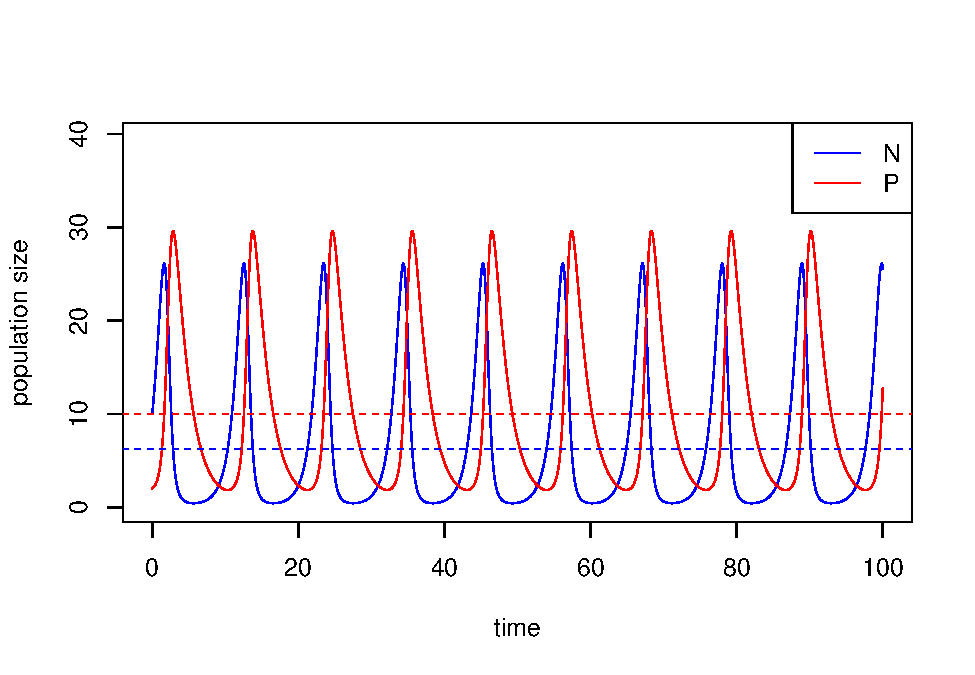
\includegraphics{bookdown-demo_files/figure-latex/unnamed-chunk-24-1.pdf}

\begin{Shaded}
\begin{Highlighting}[]
\CommentTok{### Visualization -- state-space diagram}
\KeywordTok{plot}\NormalTok{(N }\OperatorTok{~}\StringTok{ }\NormalTok{P, }\DataTypeTok{data =}\NormalTok{ pop_size, }\DataTypeTok{type =} \StringTok{"l"}\NormalTok{)}
\KeywordTok{points}\NormalTok{(parms[}\DecValTok{4}\NormalTok{]}\OperatorTok{/}\NormalTok{(parms[}\DecValTok{3}\NormalTok{] }\OperatorTok{*}\StringTok{ }\NormalTok{parms[}\DecValTok{2}\NormalTok{]), parms[}\DecValTok{1}\NormalTok{] }\OperatorTok{/}\StringTok{ }\NormalTok{parms[}\DecValTok{2}\NormalTok{]) }\CommentTok{# equilibrium}
\end{Highlighting}
\end{Shaded}

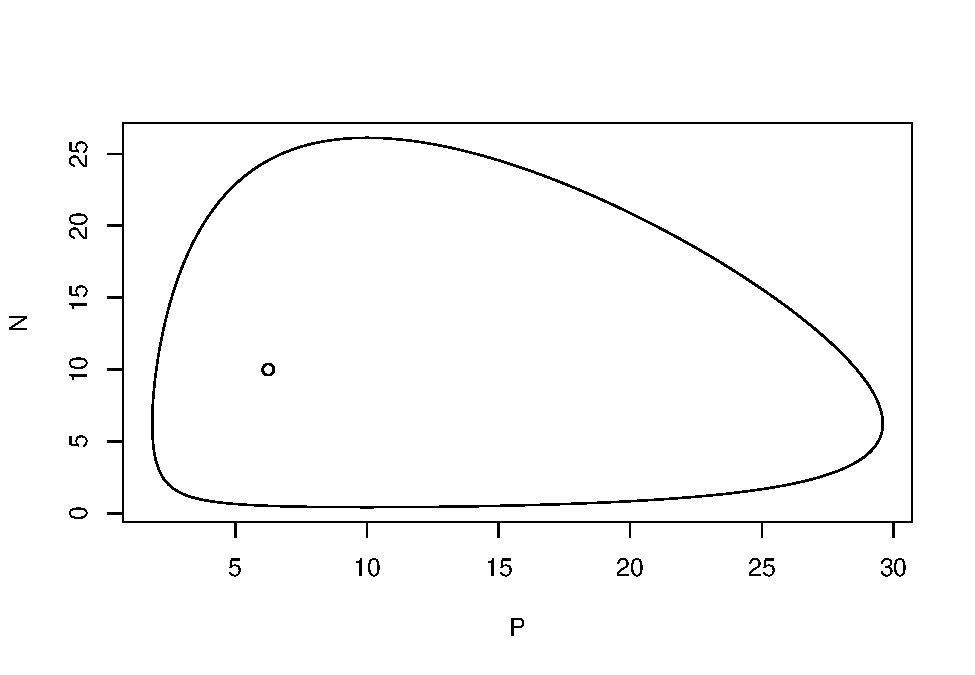
\includegraphics{bookdown-demo_files/figure-latex/unnamed-chunk-24-2.pdf}

What is the relationship between the \textbf{long-term average} of the cycle and the originally-expected equilibrium? To calculate long-term average, we need to find out the period of the cycle and then calculate the average population size within a period. The period of the cycle may be derived from the distance between peaks in the dynamics shown above, or by some algorithms, e.g.~\texttt{pracma::findpeaks}.

\textbf{Part 2: Time-scale separation}

Time-scale separation is a useful technique to reduce the dimension of the model system, where some state variables are assumed to operate at a much shorter time scale (i.e., fast variables) compared with the others (i.e., slow variables). The fast variables will be attracted rapidly to their new equilibrium in response to a slight change in the slow variables, such that the slow variables can be viewed as ``constants'' from the perspective of fast variables (and the fast variable will always be at its quasi-equilibrium from the perspective of the slow variable).

Here, we are going to use the Lotka-Volterra model with logistic prey growth to demonstrate the time-scale separation technique:

\begin{align*}
\frac {dN}{dt} &= rN(1-\frac{N}{K})-aNP\\
\frac {dP}{dt} &= eaNP-dP
\end{align*}

The ZNGIs of \(N\) are \(N = 0\) and \(r(1-\frac{N}{K}) - aP = 0\) and the ZNGIs of \(P\) are \(P = 0\) and \(eaN = d\) in this model.

We treat \textbf{prey as a fast variable and predator as a slow variable}. First, we find the quasi-equilibrium \(\widehat{N}\) of prey by setting the prey equation to zero:

\[\widehat{N} = K(1-\frac{aP}{r})\]

And then we plug \(\widehat{N}\) into predator equation:

\[\frac {dP}{dt} = (eaK-d)P(1-\frac{eaK(\frac{a}{r})}{eaK-d}P)\]

One simple way to achieve time-scale separation in this model is to increase the prey growth rate so that prey will grow much faster than predator, mimicking the shorter generation time of prey relative to that of predator.

\begin{Shaded}
\begin{Highlighting}[]
\KeywordTok{library}\NormalTok{(deSolve)}

\NormalTok{Prey_logistic_model <-}\StringTok{ }\ControlFlowTok{function}\NormalTok{(times, state, parms) \{}
  \KeywordTok{with}\NormalTok{(}\KeywordTok{as.list}\NormalTok{(}\KeywordTok{c}\NormalTok{(state, parms)), \{}
\NormalTok{    dN_dt =}\StringTok{ }\NormalTok{r}\OperatorTok{*}\NormalTok{N}\OperatorTok{*}\NormalTok{(}\DecValTok{1}\OperatorTok{-}\NormalTok{(N}\OperatorTok{/}\NormalTok{K))}\OperatorTok{-}\NormalTok{a}\OperatorTok{*}\NormalTok{N}\OperatorTok{*}\NormalTok{P}
\NormalTok{    dP_dt =}\StringTok{ }\NormalTok{e}\OperatorTok{*}\NormalTok{a}\OperatorTok{*}\NormalTok{N}\OperatorTok{*}\NormalTok{P}\OperatorTok{-}\NormalTok{d}\OperatorTok{*}\NormalTok{P}
    \KeywordTok{return}\NormalTok{(}\KeywordTok{list}\NormalTok{(}\KeywordTok{c}\NormalTok{(dN_dt, dP_dt)))}
\NormalTok{  \})}
\NormalTok{\}}

\NormalTok{times <-}\StringTok{ }\KeywordTok{seq}\NormalTok{(}\DecValTok{0}\NormalTok{, }\DecValTok{100}\NormalTok{, }\DataTypeTok{by =} \FloatTok{0.01}\NormalTok{)}
\NormalTok{state <-}\StringTok{ }\KeywordTok{c}\NormalTok{(}\DataTypeTok{N =} \DecValTok{40}\NormalTok{, }\DataTypeTok{P =} \DecValTok{20}\NormalTok{)}
\NormalTok{parms <-}\StringTok{ }\KeywordTok{c}\NormalTok{(}\DataTypeTok{r =} \DecValTok{40}\NormalTok{, }\DataTypeTok{K =} \DecValTok{60}\NormalTok{, }\DataTypeTok{a =} \FloatTok{0.1}\NormalTok{, }\DataTypeTok{e =} \FloatTok{0.1}\NormalTok{, }\DataTypeTok{d =} \FloatTok{0.5}\NormalTok{)  }\CommentTok{# r is chosen to be sufficiently large for time-scale separation}

\NormalTok{pop_size <-}\StringTok{ }\KeywordTok{ode}\NormalTok{(}\DataTypeTok{func =}\NormalTok{ Prey_logistic_model, }\DataTypeTok{times =}\NormalTok{ times, }\DataTypeTok{y =}\NormalTok{ state, }\DataTypeTok{parms =}\NormalTok{ parms)}
\end{Highlighting}
\end{Shaded}

Under time-scale separation, population of prey rapidly becomes stable and predator exhibits a logistic growth. We show these by the trajectories of \(P\) and \(N\) over time.

\begin{Shaded}
\begin{Highlighting}[]
\CommentTok{# population trajectories}
\KeywordTok{plot}\NormalTok{(}\KeywordTok{c}\NormalTok{(}\DecValTok{0}\NormalTok{, }\KeywordTok{max}\NormalTok{(times)), }\KeywordTok{c}\NormalTok{(}\DecValTok{0}\NormalTok{, }\KeywordTok{max}\NormalTok{(pop_size[, }\KeywordTok{c}\NormalTok{(}\StringTok{"N"}\NormalTok{, }\StringTok{"P"}\NormalTok{)] }\OperatorTok{+}\StringTok{ }\DecValTok{10}\NormalTok{)), }\DataTypeTok{type =} \StringTok{"n"}\NormalTok{, }\DataTypeTok{xlab =} \StringTok{"time"}\NormalTok{, }\DataTypeTok{ylab =} \StringTok{"population size"}\NormalTok{)}
\KeywordTok{lines}\NormalTok{(N }\OperatorTok{~}\StringTok{ }\NormalTok{time, }\DataTypeTok{data =}\NormalTok{ pop_size, }\DataTypeTok{col =} \StringTok{"blue"}\NormalTok{) }\CommentTok{# dynamics of N}
\KeywordTok{lines}\NormalTok{(P }\OperatorTok{~}\StringTok{ }\NormalTok{time, }\DataTypeTok{data =}\NormalTok{ pop_size, }\DataTypeTok{col =} \StringTok{"red"}\NormalTok{) }\CommentTok{# dynamics of P}
\KeywordTok{legend}\NormalTok{(}\StringTok{"topright"}\NormalTok{, }\DataTypeTok{legend =} \KeywordTok{c}\NormalTok{(}\StringTok{"N"}\NormalTok{, }\StringTok{"P"}\NormalTok{), }\DataTypeTok{col =} \KeywordTok{c}\NormalTok{(}\StringTok{"blue"}\NormalTok{, }\StringTok{"red"}\NormalTok{), }\DataTypeTok{lty =} \DecValTok{1}\NormalTok{)}
\end{Highlighting}
\end{Shaded}

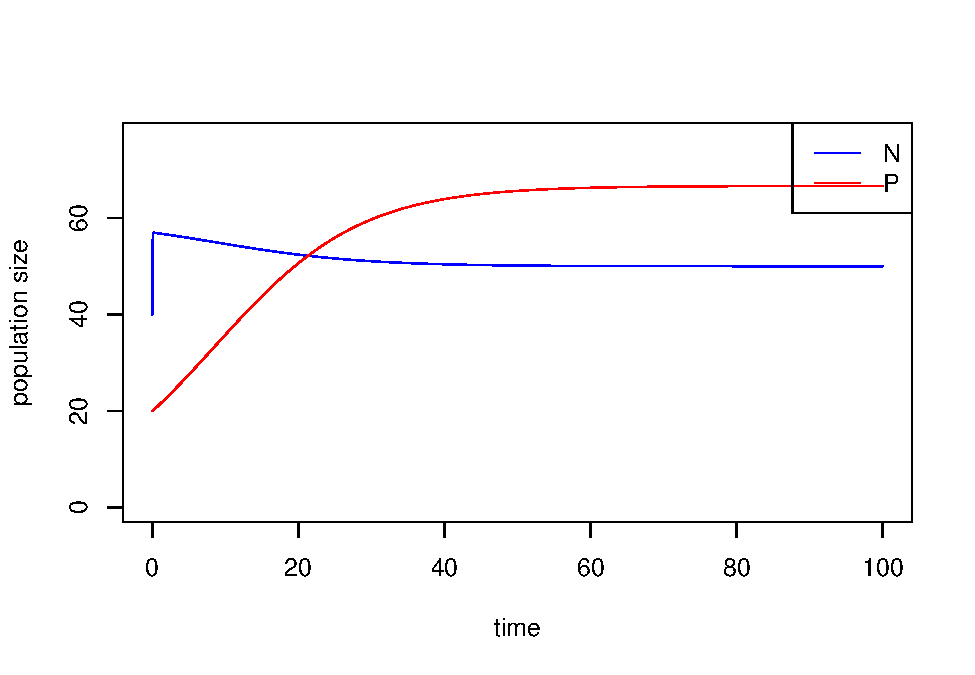
\includegraphics{bookdown-demo_files/figure-latex/unnamed-chunk-26-1.pdf}

Since \(N\) is a fast variable, it will immediately achieve the its ZNGI on the state-space diagram.

\begin{Shaded}
\begin{Highlighting}[]
\CommentTok{# state-space diagram}
\KeywordTok{plot}\NormalTok{(}\KeywordTok{c}\NormalTok{(}\DecValTok{0}\NormalTok{, }\KeywordTok{max}\NormalTok{(pop_size[, }\StringTok{"N"}\NormalTok{])), }\KeywordTok{c}\NormalTok{(}\DecValTok{0}\NormalTok{, }\KeywordTok{max}\NormalTok{(pop_size[, }\StringTok{"P"}\NormalTok{])), }\DataTypeTok{type =} \StringTok{"n"}\NormalTok{, }\DataTypeTok{xlab =} \StringTok{"N"}\NormalTok{, }\DataTypeTok{ylab =} \StringTok{"P"}\NormalTok{)}
\KeywordTok{abline}\NormalTok{(}\DataTypeTok{v =} \DecValTok{0}\NormalTok{, }\DataTypeTok{col =} \StringTok{"blue"}\NormalTok{) }\CommentTok{# ZNGI of N}
\KeywordTok{abline}\NormalTok{(}\DataTypeTok{a =}\NormalTok{ parms[}\DecValTok{1}\NormalTok{]}\OperatorTok{/}\NormalTok{parms[}\DecValTok{3}\NormalTok{], }\DataTypeTok{b =} \OperatorTok{-}\NormalTok{parms[}\DecValTok{1}\NormalTok{]}\OperatorTok{/}\NormalTok{(parms[}\DecValTok{3}\NormalTok{]}\OperatorTok{*}\NormalTok{parms[}\DecValTok{2}\NormalTok{]), }\DataTypeTok{col =} \StringTok{"blue"}\NormalTok{) }\CommentTok{# ZNGI of N}
\KeywordTok{abline}\NormalTok{(}\DataTypeTok{h =} \DecValTok{0}\NormalTok{, }\DataTypeTok{col =} \StringTok{"red"}\NormalTok{) }\CommentTok{# ZNGI of P}
\KeywordTok{abline}\NormalTok{(}\DataTypeTok{v =}\NormalTok{ parms[}\DecValTok{5}\NormalTok{]}\OperatorTok{/}\NormalTok{(parms[}\DecValTok{4}\NormalTok{]}\OperatorTok{*}\NormalTok{parms[}\DecValTok{3}\NormalTok{]), }\DataTypeTok{col =} \StringTok{"red"}\NormalTok{) }\CommentTok{# ZNGI of P}
\KeywordTok{points}\NormalTok{(P }\OperatorTok{~}\StringTok{ }\NormalTok{N, }\DataTypeTok{data =}\NormalTok{ pop_size, }\DataTypeTok{col =} \StringTok{"gray"}\NormalTok{)}
\end{Highlighting}
\end{Shaded}

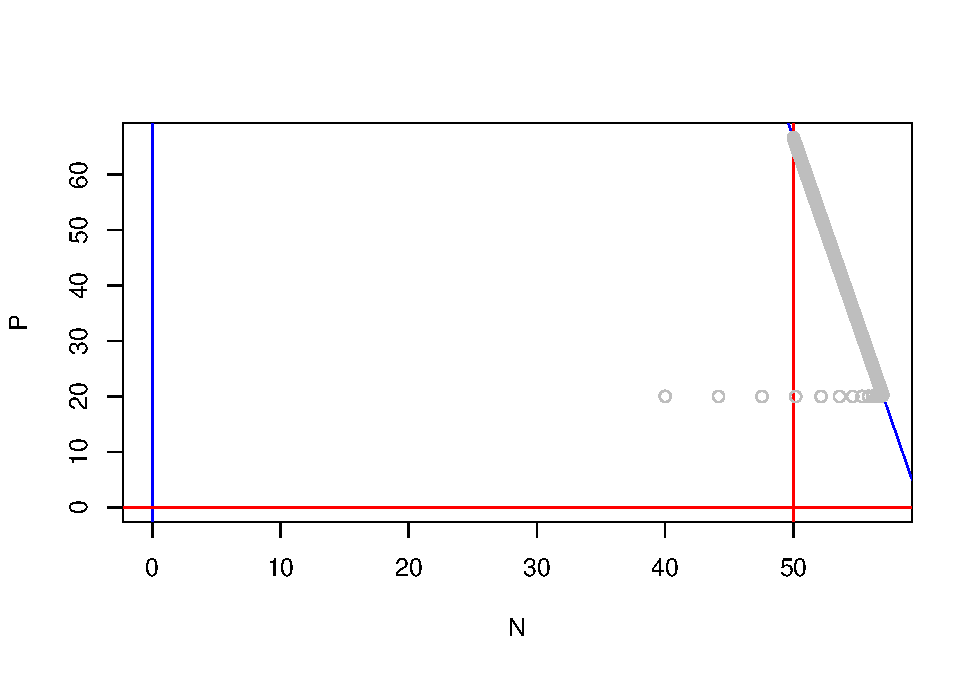
\includegraphics{bookdown-demo_files/figure-latex/unnamed-chunk-27-1.pdf}

Play with the growth rate \(r\) from small to large values and see how the trajectory of prey and predator moves along the state-space.

Shiny app is credit to \href{https://genchanghsu.github.io/index.html}{Gen-Chang Hsu}

\hypertarget{week-11---no-class-due-to-ntu-anniversary}{%
\chapter*{Week 11 - No class due to NTU anniversary}\label{week-11---no-class-due-to-ntu-anniversary}}
\addcontentsline{toc}{chapter}{Week 11 - No class due to NTU anniversary}

\hypertarget{week-12---rosenzweig-macarthur-predator-prey-model-and-mays-complexity-stability-relationship}{%
\chapter*{Week 12 - Rosenzweig-MacArthur predator-prey model and May's complexity-stability relationship}\label{week-12---rosenzweig-macarthur-predator-prey-model-and-mays-complexity-stability-relationship}}
\addcontentsline{toc}{chapter}{Week 12 - Rosenzweig-MacArthur predator-prey model and May's complexity-stability relationship}

\textbf{Part 1: Rosenzweig--MacArthur predator--prey model}

In this lab we are going to analyze the Rosenzweig--MacArthur predator--prey model:

\begin{align*}
\frac {dN}{dt} &= rN(1-\frac{N}{K})-a\frac{N}{1+ahN}P\\
\frac {dP}{dt} &= ea\frac{N}{1+ahN}P-dP,\\
\end{align*}
where \(r\) is the intrinsic growth rate of prey, \(K\) is the carrying capacity of prey, \(a\) is the rate of prey being consumed by predator, \(h\) is the handling time of predator, \(e\) is the assimilation rate of predation and \(d\) is the mortality rate of predator. The ZNGIs of \(N\) are
\[
N = 0 \text{ and } P = \frac{r}{a}(1-\frac{N}{K})(1+ahN)
\]
and the ZNGIs of \(P\) are
\[
P = 0 \text{ and } N = \frac{d}{a(e-dh)}
\]
The coexistence equilibrium is \(E_{np} = \left(N^* = \frac{d}{a(e-dh)}, P^* = \frac{r}{a}(1-\frac{N^*}{K})(1+ahN^*)\right)\).

Please simulate the model using the parameter set (\(N_0\) = 5, \(P_0\) = 2, \(r\) = 1.0, \(K\) = 5.0, \(a\) = 1.3, \(h\) = 0.9, \(e\) = 0.6, \(d\) = 0.5) and plot the population trajectories of predator and prey as well as show their population dynamics in the state-space diagram.

\begin{Shaded}
\begin{Highlighting}[]
\KeywordTok{library}\NormalTok{(deSolve)}

\CommentTok{### Model specification}
\NormalTok{RM_predation_model <-}\StringTok{ }\ControlFlowTok{function}\NormalTok{(times, state, parms) \{}
  \KeywordTok{with}\NormalTok{(}\KeywordTok{as.list}\NormalTok{(}\KeywordTok{c}\NormalTok{(state, parms)), \{}
\NormalTok{    dN_dt =}\StringTok{ }\NormalTok{r}\OperatorTok{*}\NormalTok{N}\OperatorTok{*}\NormalTok{(}\DecValTok{1}\OperatorTok{-}\NormalTok{(N}\OperatorTok{/}\NormalTok{K))}\OperatorTok{-}\NormalTok{(a}\OperatorTok{*}\NormalTok{N}\OperatorTok{/}\NormalTok{(}\DecValTok{1}\OperatorTok{+}\NormalTok{a}\OperatorTok{*}\NormalTok{h}\OperatorTok{*}\NormalTok{N))}\OperatorTok{*}\NormalTok{P}
\NormalTok{    dP_dt =}\StringTok{ }\NormalTok{e}\OperatorTok{*}\NormalTok{(a}\OperatorTok{*}\NormalTok{N}\OperatorTok{/}\NormalTok{(}\DecValTok{1}\OperatorTok{+}\NormalTok{a}\OperatorTok{*}\NormalTok{h}\OperatorTok{*}\NormalTok{N))}\OperatorTok{*}\NormalTok{P}\OperatorTok{-}\NormalTok{d}\OperatorTok{*}\NormalTok{P}
    \KeywordTok{return}\NormalTok{(}\KeywordTok{list}\NormalTok{(}\KeywordTok{c}\NormalTok{(dN_dt, dP_dt)))  }
\NormalTok{  \})}
\NormalTok{\}}

\CommentTok{### Model parameters}
\NormalTok{times <-}\StringTok{ }\KeywordTok{seq}\NormalTok{(}\DecValTok{0}\NormalTok{, }\DecValTok{200}\NormalTok{, }\DataTypeTok{by =} \FloatTok{0.01}\NormalTok{)  }
\NormalTok{state <-}\StringTok{ }\KeywordTok{c}\NormalTok{(}\DataTypeTok{N =} \DecValTok{5}\NormalTok{, }\DataTypeTok{P =} \DecValTok{2}\NormalTok{)  }
\NormalTok{parms <-}\StringTok{ }\KeywordTok{c}\NormalTok{(}\DataTypeTok{r =} \FloatTok{1.0}\NormalTok{, }\DataTypeTok{K =} \FloatTok{5.0}\NormalTok{, }\DataTypeTok{a =} \FloatTok{1.3}\NormalTok{, }\DataTypeTok{h =} \FloatTok{0.9}\NormalTok{, }\DataTypeTok{e =} \FloatTok{0.6}\NormalTok{, }\DataTypeTok{d =} \FloatTok{0.5}\NormalTok{) }

\CommentTok{### Model application}
\NormalTok{pop_size <-}\StringTok{ }\KeywordTok{ode}\NormalTok{(}\DataTypeTok{func =}\NormalTok{ RM_predation_model, }\DataTypeTok{times =}\NormalTok{ times, }\DataTypeTok{y =}\NormalTok{ state, }\DataTypeTok{parms =}\NormalTok{ parms)}

\CommentTok{### equilibrium}
\NormalTok{E_np <-}\StringTok{ }\KeywordTok{with}\NormalTok{(}\KeywordTok{as.list}\NormalTok{(parms), }
             \KeywordTok{c}\NormalTok{(}\DataTypeTok{N =}\NormalTok{ d}\OperatorTok{/}\NormalTok{(a}\OperatorTok{*}\NormalTok{(e}\OperatorTok{-}\NormalTok{d}\OperatorTok{*}\NormalTok{h)),}
               \DataTypeTok{P =}\NormalTok{ r}\OperatorTok{/}\NormalTok{a}\OperatorTok{*}\NormalTok{(}\DecValTok{1}\OperatorTok{-}\NormalTok{d}\OperatorTok{/}\NormalTok{(a}\OperatorTok{*}\NormalTok{(e}\OperatorTok{-}\NormalTok{d}\OperatorTok{*}\NormalTok{h))}\OperatorTok{/}\NormalTok{K)}\OperatorTok{*}\NormalTok{(}\DecValTok{1}\OperatorTok{+}\NormalTok{a}\OperatorTok{*}\NormalTok{h}\OperatorTok{*}\NormalTok{d}\OperatorTok{/}\NormalTok{(a}\OperatorTok{*}\NormalTok{(e}\OperatorTok{-}\NormalTok{d}\OperatorTok{*}\NormalTok{h)))))}


\CommentTok{### Visualize the population dynamics}
\CommentTok{# population trajectories}
\KeywordTok{plot}\NormalTok{(}\KeywordTok{c}\NormalTok{(}\DecValTok{0}\NormalTok{, }\KeywordTok{max}\NormalTok{(times)), }\KeywordTok{c}\NormalTok{(}\DecValTok{0}\NormalTok{, }\KeywordTok{max}\NormalTok{(pop_size[, }\KeywordTok{c}\NormalTok{(}\StringTok{"N"}\NormalTok{, }\StringTok{"P"}\NormalTok{)])), }\DataTypeTok{type =} \StringTok{"n"}\NormalTok{, }\DataTypeTok{xlab =} \StringTok{"time"}\NormalTok{, }\DataTypeTok{ylab =} \StringTok{"population size"}\NormalTok{)}
\KeywordTok{lines}\NormalTok{(N }\OperatorTok{~}\StringTok{ }\NormalTok{time, }\DataTypeTok{data =}\NormalTok{ pop_size, }\DataTypeTok{col =} \StringTok{"blue"}\NormalTok{) }\CommentTok{# dynamics of N}
\KeywordTok{lines}\NormalTok{(P }\OperatorTok{~}\StringTok{ }\NormalTok{time, }\DataTypeTok{data =}\NormalTok{ pop_size, }\DataTypeTok{col =} \StringTok{"red"}\NormalTok{) }\CommentTok{# dynamics of P}
\KeywordTok{legend}\NormalTok{(}\StringTok{"topright"}\NormalTok{, }\DataTypeTok{legend =} \KeywordTok{c}\NormalTok{(}\StringTok{"N"}\NormalTok{, }\StringTok{"P"}\NormalTok{), }\DataTypeTok{col =} \KeywordTok{c}\NormalTok{(}\StringTok{"blue"}\NormalTok{, }\StringTok{"red"}\NormalTok{), }\DataTypeTok{lty =} \DecValTok{1}\NormalTok{)}
\end{Highlighting}
\end{Shaded}

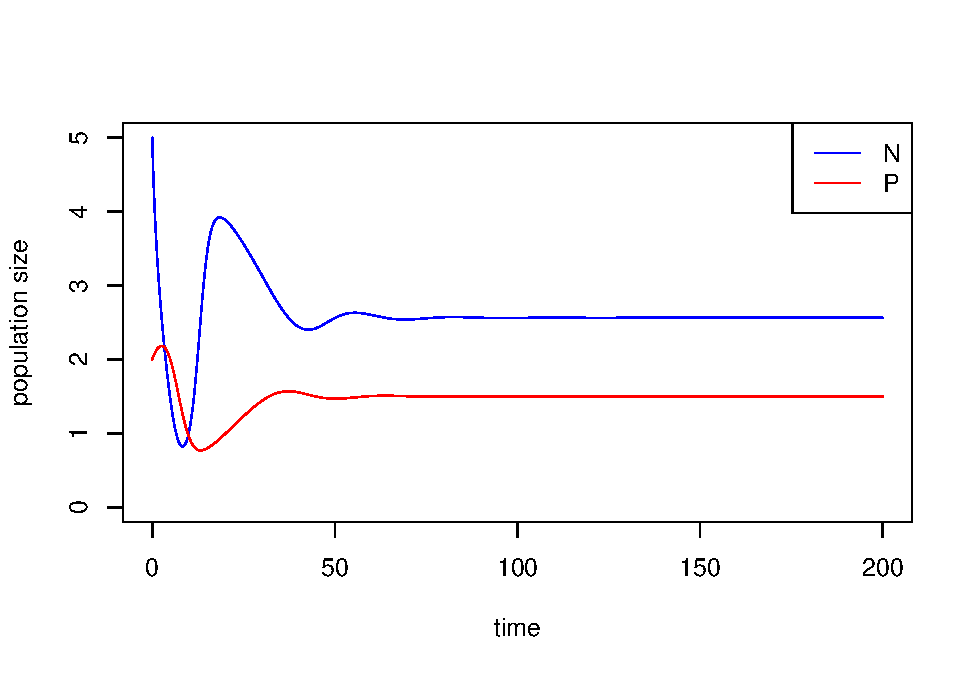
\includegraphics{bookdown-demo_files/figure-latex/unnamed-chunk-29-1.pdf}

\begin{Shaded}
\begin{Highlighting}[]
\CommentTok{# state-space diagram}
\NormalTok{max_P <-}\StringTok{ }\KeywordTok{max}\NormalTok{(pop_size[ ,}\StringTok{"P"}\NormalTok{])}
\NormalTok{max_N <-}\StringTok{ }\KeywordTok{max}\NormalTok{(pop_size[ ,}\StringTok{"N"}\NormalTok{])}
\KeywordTok{plot}\NormalTok{(P }\OperatorTok{~}\StringTok{ }\NormalTok{N, }\DataTypeTok{data =}\NormalTok{ pop_size, }\DataTypeTok{type =} \StringTok{"l"}\NormalTok{, }\DataTypeTok{xlim =} \KeywordTok{c}\NormalTok{(}\DecValTok{0}\NormalTok{, max_N}\OperatorTok{*}\FloatTok{1.2}\NormalTok{), }\DataTypeTok{ylim =} \KeywordTok{c}\NormalTok{(}\DecValTok{0}\NormalTok{, max_P}\OperatorTok{*}\FloatTok{1.2}\NormalTok{))}
\KeywordTok{points}\NormalTok{(E_np[}\StringTok{"P"}\NormalTok{] }\OperatorTok{~}\StringTok{ }\NormalTok{E_np[}\StringTok{"N"}\NormalTok{], }\DataTypeTok{pch =} \DecValTok{16}\NormalTok{) }\CommentTok{# equilibrium }
\KeywordTok{with}\NormalTok{(}\KeywordTok{as.list}\NormalTok{(parms), \{}
  \CommentTok{# ZNGIs of N}
  \KeywordTok{abline}\NormalTok{(}\DataTypeTok{v =} \DecValTok{0}\NormalTok{, }\DataTypeTok{col =} \StringTok{"blue"}\NormalTok{)}
  \KeywordTok{curve}\NormalTok{(r}\OperatorTok{/}\NormalTok{a}\OperatorTok{*}\NormalTok{(}\DecValTok{1}\OperatorTok{-}\NormalTok{x}\OperatorTok{/}\NormalTok{K)}\OperatorTok{*}\NormalTok{(}\DecValTok{1}\OperatorTok{+}\NormalTok{a}\OperatorTok{*}\NormalTok{h}\OperatorTok{*}\NormalTok{x), }\DataTypeTok{from =} \DecValTok{-2}\NormalTok{, }\DataTypeTok{to =}\NormalTok{ K}\OperatorTok{+}\DecValTok{2}\NormalTok{, }\DataTypeTok{col =} \StringTok{"blue"}\NormalTok{, }\DataTypeTok{add =}\NormalTok{ T)}
  \CommentTok{# ZNGIs of P}
  \KeywordTok{abline}\NormalTok{(}\DataTypeTok{h =} \DecValTok{0}\NormalTok{, }\DataTypeTok{col =} \StringTok{"red"}\NormalTok{)}
  \KeywordTok{abline}\NormalTok{(}\DataTypeTok{v =}\NormalTok{ d}\OperatorTok{/}\NormalTok{(a}\OperatorTok{*}\NormalTok{(e}\OperatorTok{-}\NormalTok{d}\OperatorTok{*}\NormalTok{h)), }\DataTypeTok{col =} \StringTok{"red"}\NormalTok{)}
\NormalTok{  \}) }
\KeywordTok{legend}\NormalTok{(}\StringTok{"topright"}\NormalTok{, }\DataTypeTok{legend =} \KeywordTok{c}\NormalTok{(}\StringTok{"ZNGIs of N"}\NormalTok{, }\StringTok{"ZNGIs of P"}\NormalTok{), }\DataTypeTok{col =} \KeywordTok{c}\NormalTok{(}\StringTok{"blue"}\NormalTok{, }\StringTok{"red"}\NormalTok{), }\DataTypeTok{lty =} \DecValTok{1}\NormalTok{)}
\end{Highlighting}
\end{Shaded}

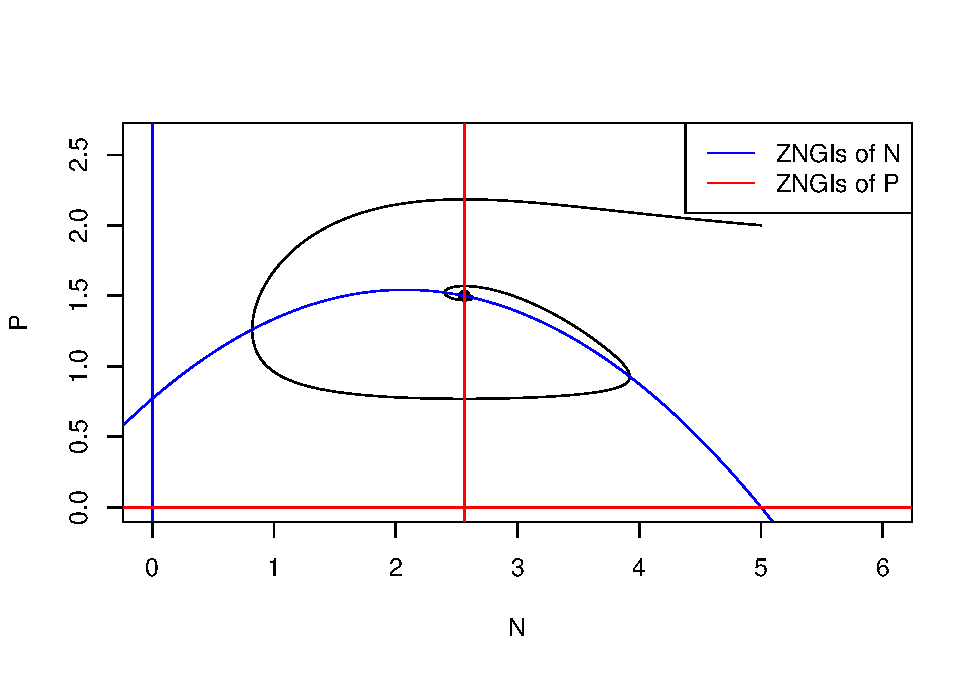
\includegraphics{bookdown-demo_files/figure-latex/unnamed-chunk-29-2.pdf}

\emph{Remark: \texttt{with()} is a function that you can load the value in the object without subsetting.}

Now we increase the carry capacity \(K\) to show the \textbf{paradox of enrichment}. Let's consider \(K = 7\) with other parameters fixed.

\begin{Shaded}
\begin{Highlighting}[]
\CommentTok{### Model parameters}
\NormalTok{times <-}\StringTok{ }\KeywordTok{seq}\NormalTok{(}\DecValTok{0}\NormalTok{, }\DecValTok{200}\NormalTok{, }\DataTypeTok{by =} \FloatTok{0.01}\NormalTok{)  }
\NormalTok{state <-}\StringTok{ }\KeywordTok{c}\NormalTok{(}\DataTypeTok{N =} \DecValTok{5}\NormalTok{, }\DataTypeTok{P =} \DecValTok{2}\NormalTok{)  }
\NormalTok{parms <-}\StringTok{ }\KeywordTok{c}\NormalTok{(}\DataTypeTok{r =} \FloatTok{1.0}\NormalTok{, }\DataTypeTok{K =} \FloatTok{7.0}\NormalTok{, }\DataTypeTok{a =} \FloatTok{1.3}\NormalTok{, }\DataTypeTok{h =} \FloatTok{0.9}\NormalTok{, }\DataTypeTok{e =} \FloatTok{0.6}\NormalTok{, }\DataTypeTok{d =} \FloatTok{0.5}\NormalTok{) }

\CommentTok{### Model application}
\NormalTok{pop_size <-}\StringTok{ }\KeywordTok{ode}\NormalTok{(}\DataTypeTok{func =}\NormalTok{ RM_predation_model, }\DataTypeTok{times =}\NormalTok{ times, }\DataTypeTok{y =}\NormalTok{ state, }\DataTypeTok{parms =}\NormalTok{ parms)}

\CommentTok{### equilibrium}
\NormalTok{E_np <-}\StringTok{ }\KeywordTok{with}\NormalTok{(}\KeywordTok{as.list}\NormalTok{(parms), }
             \KeywordTok{c}\NormalTok{(}\DataTypeTok{N =}\NormalTok{ d}\OperatorTok{/}\NormalTok{(a}\OperatorTok{*}\NormalTok{(e}\OperatorTok{-}\NormalTok{d}\OperatorTok{*}\NormalTok{h)),}
               \DataTypeTok{P =}\NormalTok{ r}\OperatorTok{/}\NormalTok{a}\OperatorTok{*}\NormalTok{(}\DecValTok{1}\OperatorTok{-}\NormalTok{d}\OperatorTok{/}\NormalTok{(a}\OperatorTok{*}\NormalTok{(e}\OperatorTok{-}\NormalTok{d}\OperatorTok{*}\NormalTok{h))}\OperatorTok{/}\NormalTok{K)}\OperatorTok{*}\NormalTok{(}\DecValTok{1}\OperatorTok{+}\NormalTok{a}\OperatorTok{*}\NormalTok{h}\OperatorTok{*}\NormalTok{d}\OperatorTok{/}\NormalTok{(a}\OperatorTok{*}\NormalTok{(e}\OperatorTok{-}\NormalTok{d}\OperatorTok{*}\NormalTok{h)))))}
\end{Highlighting}
\end{Shaded}

The population size of \(N\) and \(P\) do not stay at the equilibrium but cycle.

\begin{Shaded}
\begin{Highlighting}[]
\CommentTok{### Visualize the population dynamics}
\CommentTok{# population trajectories}
\KeywordTok{plot}\NormalTok{(}\KeywordTok{c}\NormalTok{(}\DecValTok{0}\NormalTok{, }\KeywordTok{max}\NormalTok{(times)), }\KeywordTok{c}\NormalTok{(}\DecValTok{0}\NormalTok{, }\KeywordTok{max}\NormalTok{(pop_size[, }\KeywordTok{c}\NormalTok{(}\StringTok{"N"}\NormalTok{, }\StringTok{"P"}\NormalTok{)])}\OperatorTok{*}\FloatTok{1.2}\NormalTok{), }\DataTypeTok{type =} \StringTok{"n"}\NormalTok{, }\DataTypeTok{xlab =} \StringTok{"time"}\NormalTok{, }\DataTypeTok{ylab =} \StringTok{"population size"}\NormalTok{)}
\KeywordTok{lines}\NormalTok{(N }\OperatorTok{~}\StringTok{ }\NormalTok{time, }\DataTypeTok{data =}\NormalTok{ pop_size, }\DataTypeTok{col =} \StringTok{"blue"}\NormalTok{) }\CommentTok{# dynamics of N}
\KeywordTok{lines}\NormalTok{(P }\OperatorTok{~}\StringTok{ }\NormalTok{time, }\DataTypeTok{data =}\NormalTok{ pop_size, }\DataTypeTok{col =} \StringTok{"red"}\NormalTok{) }\CommentTok{# dynamics of P}
\KeywordTok{legend}\NormalTok{(}\StringTok{"topright"}\NormalTok{, }\DataTypeTok{legend =} \KeywordTok{c}\NormalTok{(}\StringTok{"N"}\NormalTok{, }\StringTok{"P"}\NormalTok{), }\DataTypeTok{col =} \KeywordTok{c}\NormalTok{(}\StringTok{"blue"}\NormalTok{, }\StringTok{"red"}\NormalTok{), }\DataTypeTok{lty =} \DecValTok{1}\NormalTok{)}
\end{Highlighting}
\end{Shaded}

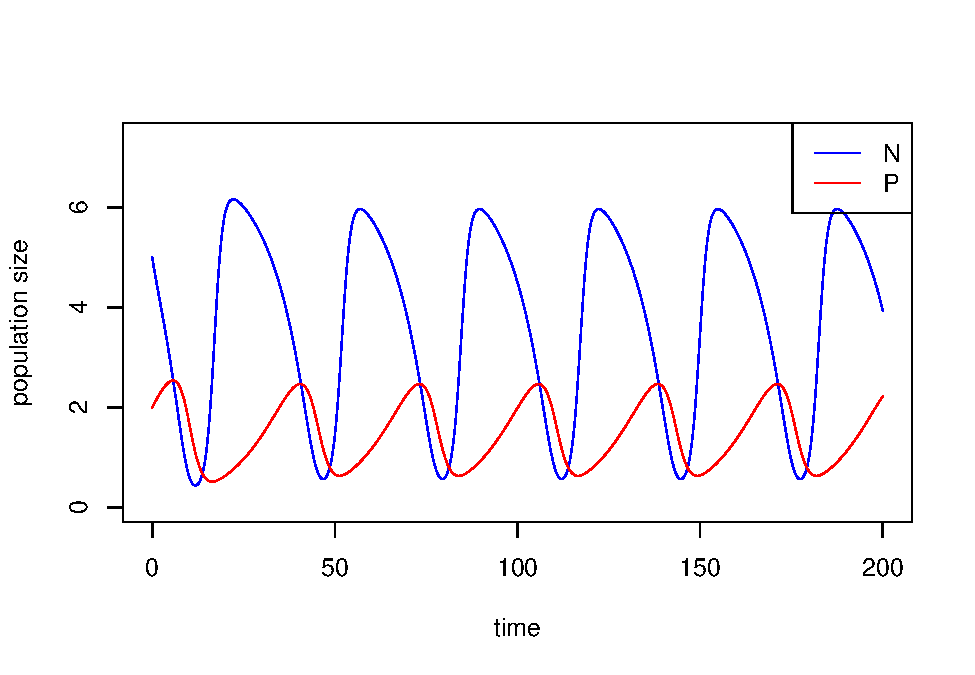
\includegraphics{bookdown-demo_files/figure-latex/unnamed-chunk-31-1.pdf}

\begin{Shaded}
\begin{Highlighting}[]
\CommentTok{# state-space diagram}
\NormalTok{max_P <-}\StringTok{ }\KeywordTok{max}\NormalTok{(pop_size[ ,}\StringTok{"P"}\NormalTok{])}
\NormalTok{max_N <-}\StringTok{ }\KeywordTok{max}\NormalTok{(pop_size[ ,}\StringTok{"N"}\NormalTok{])}
\KeywordTok{plot}\NormalTok{(P }\OperatorTok{~}\StringTok{ }\NormalTok{N, }\DataTypeTok{data =}\NormalTok{ pop_size, }\DataTypeTok{type =} \StringTok{"l"}\NormalTok{, }\DataTypeTok{xlim =} \KeywordTok{c}\NormalTok{(}\DecValTok{0}\NormalTok{, max_N}\OperatorTok{*}\FloatTok{1.2}\NormalTok{), }\DataTypeTok{ylim =} \KeywordTok{c}\NormalTok{(}\DecValTok{0}\NormalTok{, max_P}\OperatorTok{*}\FloatTok{1.2}\NormalTok{))}
\KeywordTok{points}\NormalTok{(E_np[}\StringTok{"P"}\NormalTok{] }\OperatorTok{~}\StringTok{ }\NormalTok{E_np[}\StringTok{"N"}\NormalTok{], }\DataTypeTok{pch =} \DecValTok{16}\NormalTok{) }\CommentTok{# equilibrium }
\KeywordTok{with}\NormalTok{(}\KeywordTok{as.list}\NormalTok{(parms), \{}
  \CommentTok{# ZNGIs of N}
  \KeywordTok{abline}\NormalTok{(}\DataTypeTok{v =} \DecValTok{0}\NormalTok{, }\DataTypeTok{col =} \StringTok{"blue"}\NormalTok{)}
  \KeywordTok{curve}\NormalTok{(r}\OperatorTok{/}\NormalTok{a}\OperatorTok{*}\NormalTok{(}\DecValTok{1}\OperatorTok{-}\NormalTok{x}\OperatorTok{/}\NormalTok{K)}\OperatorTok{*}\NormalTok{(}\DecValTok{1}\OperatorTok{+}\NormalTok{a}\OperatorTok{*}\NormalTok{h}\OperatorTok{*}\NormalTok{x), }\DataTypeTok{from =} \DecValTok{-2}\NormalTok{, }\DataTypeTok{to =}\NormalTok{ K}\OperatorTok{+}\DecValTok{2}\NormalTok{, }\DataTypeTok{col =} \StringTok{"blue"}\NormalTok{, }\DataTypeTok{add =}\NormalTok{ T)}
  \CommentTok{# ZNGIs of P}
  \KeywordTok{abline}\NormalTok{(}\DataTypeTok{h =} \DecValTok{0}\NormalTok{, }\DataTypeTok{col =} \StringTok{"red"}\NormalTok{)}
  \KeywordTok{abline}\NormalTok{(}\DataTypeTok{v =}\NormalTok{ d}\OperatorTok{/}\NormalTok{(a}\OperatorTok{*}\NormalTok{(e}\OperatorTok{-}\NormalTok{d}\OperatorTok{*}\NormalTok{h)), }\DataTypeTok{col =} \StringTok{"red"}\NormalTok{)}
\NormalTok{  \}) }
\KeywordTok{legend}\NormalTok{(}\StringTok{"topright"}\NormalTok{, }\DataTypeTok{legend =} \KeywordTok{c}\NormalTok{(}\StringTok{"ZNGIs of N"}\NormalTok{, }\StringTok{"ZNGIs of P"}\NormalTok{), }\DataTypeTok{col =} \KeywordTok{c}\NormalTok{(}\StringTok{"blue"}\NormalTok{, }\StringTok{"red"}\NormalTok{), }\DataTypeTok{lty =} \DecValTok{1}\NormalTok{)}
\end{Highlighting}
\end{Shaded}

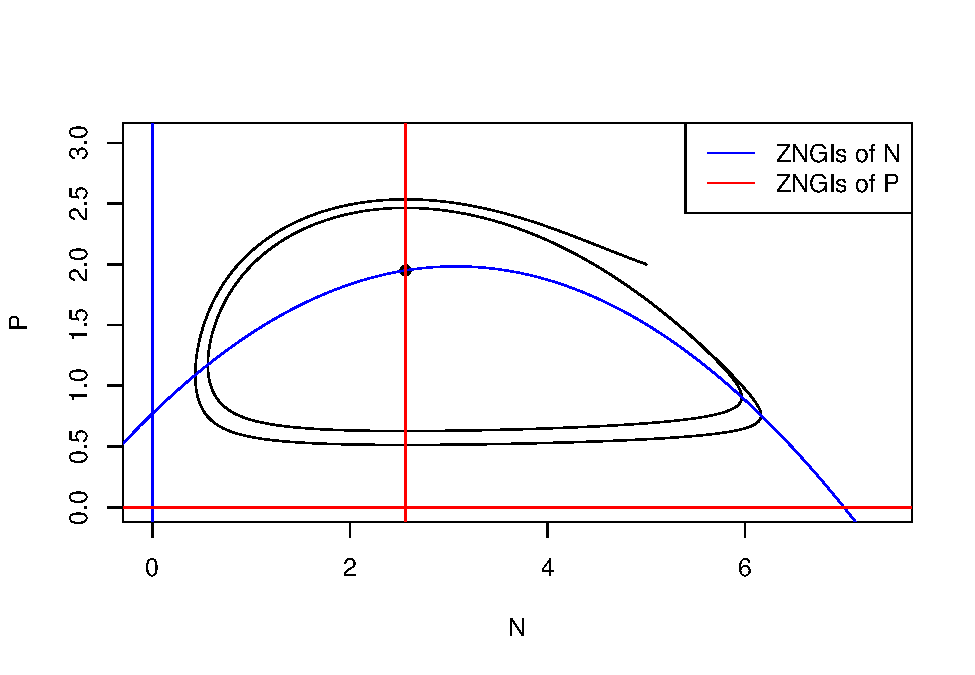
\includegraphics{bookdown-demo_files/figure-latex/unnamed-chunk-31-2.pdf}

Do the \textbf{long-term average} of the population size equal to the equilibrium? Let's calculate the long-term average of population size by function \texttt{pracma::findpeaks()}. It returns a matrix where each row represents one peak found. The first column gives the height, the second the position/index where the maximum is reached, the third and forth the indices of where the peak begins and ends --- in the sense of where the pattern starts and ends.

\begin{Shaded}
\begin{Highlighting}[]
\KeywordTok{library}\NormalTok{(pracma)}
\CommentTok{# find time points when local peaks occur}
\NormalTok{peaks <-}\StringTok{ }\KeywordTok{findpeaks}\NormalTok{(pop_size[, }\StringTok{"N"}\NormalTok{])[ ,}\DecValTok{2}\NormalTok{]}
\NormalTok{peaks }
\end{Highlighting}
\end{Shaded}

\begin{verbatim}
## [1]  2219  5694  8960 12225 15490 18755
\end{verbatim}

\begin{Shaded}
\begin{Highlighting}[]
\CommentTok{# get period as time between peaks }
\NormalTok{periods <-}\StringTok{ }\NormalTok{peaks[}\KeywordTok{length}\NormalTok{(peaks)] }\OperatorTok{-}\StringTok{ }\NormalTok{peaks[}\KeywordTok{length}\NormalTok{(peaks) }\OperatorTok{-}\StringTok{ }\DecValTok{1}\NormalTok{]}
\CommentTok{# long-term average of N}
\NormalTok{avg_N <-}\StringTok{ }\KeywordTok{mean}\NormalTok{(pop_size[(}\KeywordTok{length}\NormalTok{(times) }\OperatorTok{-}\StringTok{ }\NormalTok{periods }\OperatorTok{+}\StringTok{ }\DecValTok{1}\NormalTok{)}\OperatorTok{:}\KeywordTok{length}\NormalTok{(times), }\StringTok{"N"}\NormalTok{])}
\NormalTok{avg_N}
\end{Highlighting}
\end{Shaded}

\begin{verbatim}
## [1] 3.642661
\end{verbatim}

\begin{Shaded}
\begin{Highlighting}[]
\CommentTok{# long-term average of P}
\NormalTok{avg_P <-}\StringTok{ }\KeywordTok{mean}\NormalTok{(pop_size[(}\KeywordTok{length}\NormalTok{(times) }\OperatorTok{-}\StringTok{ }\NormalTok{periods }\OperatorTok{+}\StringTok{ }\DecValTok{1}\NormalTok{)}\OperatorTok{:}\KeywordTok{length}\NormalTok{(times), }\StringTok{"P"}\NormalTok{])}
\NormalTok{avg_P}
\end{Highlighting}
\end{Shaded}

\begin{verbatim}
## [1] 1.4757
\end{verbatim}

\begin{Shaded}
\begin{Highlighting}[]
\CommentTok{# equilibrium of N and P}
\NormalTok{E_np}
\end{Highlighting}
\end{Shaded}

\begin{verbatim}
##        N        P 
## 2.564103 1.949845
\end{verbatim}

We show that the the long-term average of the population size of \(N\) and \(P\) are not identical to the equilibrium of \(N\) and \(P\). In fact, the long-term average of the resource \(N\) is larger than the original equilibrium due to the fact that the per capita growth rate of the \(P\) is a concave-downward function.

What will happen if you add a perturbation to the system (i.e., change the initial conditions)? Try out different values of \(N_0\) and \(P_0\) and visualize the differences in the state-space diagram.

Shiny app is credit to \href{https://genchanghsu.github.io/index.html}{Gen-Chang Hsu}

\textbf{Part 2: May's complexity-stability relationship}

May's insight was to skip the Jacobian calculation altogether and directly consider the Jacobian matrix as a large random matrix (\(\mathbf{M}\), with elements \(m_{ij}\)) resting at a feasible equilibrium, and then the eigenvalues of the Jacobian matrix could be derived based on random matrix theory.

Let's try to recreate May's random matrix. In particular, May considered the following algorithm to build the random Jacobian matrix for \(S\) species (thereby a \(S \times S\) matrix):

\begin{itemize}
    \item For all the elements $m_{ij}$ in $\mathbf{M}$, let $m_{ij} = 0$ with probability $1-C$ and with probability $C$ be drawn from a distribution (here, let's assume a normal distribution) with mean 0 and variance $\sigma^{2}$. All $m_{ij}$ are generated independently.
    \item The diagonal elements $m_{ii}$ are then subtracted by $d$. 
\end{itemize}

\noindent Here, \(C\) represents the connectedness of the system (chance of species interacting with each other), \(\sigma^{2}\) can be considered as the realized interaction strengths, and \(d\) is the strength of self-limitation.

\begin{Shaded}
\begin{Highlighting}[]
\CommentTok{# code for building May's random matrix}
\NormalTok{BuildMay =}\StringTok{ }\ControlFlowTok{function}\NormalTok{(S, C, d, sigma)\{}
  \CommentTok{# fill the whole matrix}
\NormalTok{  entry <-}\StringTok{ }\KeywordTok{rnorm}\NormalTok{(S }\OperatorTok{*}\StringTok{ }\NormalTok{S, }\DataTypeTok{mean =} \DecValTok{0}\NormalTok{, }\DataTypeTok{sd =}\NormalTok{ sigma)}
\NormalTok{  M <-}\StringTok{ }\KeywordTok{matrix}\NormalTok{(entry, }\DataTypeTok{nrow =}\NormalTok{ S, }\DataTypeTok{ncol =}\NormalTok{ S)}
  \CommentTok{# remove connections}
\NormalTok{  remove <-}\StringTok{ }\KeywordTok{matrix}\NormalTok{(}\KeywordTok{runif}\NormalTok{(S }\OperatorTok{*}\StringTok{ }\NormalTok{S) }\OperatorTok{<=}\StringTok{ }\NormalTok{C, }\DataTypeTok{nrow =}\NormalTok{ S, }\DataTypeTok{ncol =}\NormalTok{ S)}
\NormalTok{  M <-}\StringTok{ }\NormalTok{M }\OperatorTok{*}\StringTok{ }\NormalTok{remove}

  \KeywordTok{sum}\NormalTok{(M }\OperatorTok{!=}\StringTok{ }\DecValTok{0}\NormalTok{) }\OperatorTok{/}\StringTok{ }\NormalTok{(S}\OperatorTok{*}\NormalTok{S) }\CommentTok{# should equal to C}

  \CommentTok{# substrate diagonal elements by d}
  \KeywordTok{diag}\NormalTok{(M) <-}\StringTok{ }\KeywordTok{diag}\NormalTok{(M) }\OperatorTok{-}\StringTok{ }\NormalTok{d}
  \KeywordTok{return}\NormalTok{(M)}
\NormalTok{\}}

\NormalTok{May <-}\StringTok{ }\KeywordTok{BuildMay}\NormalTok{(}\DataTypeTok{S =} \DecValTok{500}\NormalTok{, }\DataTypeTok{C =} \FloatTok{0.5}\NormalTok{, }\DataTypeTok{d =} \DecValTok{10}\NormalTok{, }\DataTypeTok{sigma =} \DecValTok{1}\NormalTok{)}
\NormalTok{EVals <-}\StringTok{ }\KeywordTok{eigen}\NormalTok{(May)}\OperatorTok{$}\NormalTok{values}
\NormalTok{Re.EVals <-}\StringTok{ }\KeywordTok{Re}\NormalTok{(EVals)}
\NormalTok{Im.EVals <-}\StringTok{ }\KeywordTok{Im}\NormalTok{(EVals)}

\KeywordTok{plot}\NormalTok{(Re.EVals, Im.EVals, }\DataTypeTok{xlab =} \StringTok{"Real part"}\NormalTok{, }\DataTypeTok{ylab =} \StringTok{"Imaginary part"}\NormalTok{)}
\KeywordTok{abline}\NormalTok{(}\DataTypeTok{v =} \DecValTok{0}\NormalTok{, }\DataTypeTok{col =} \StringTok{"red"}\NormalTok{, }\DataTypeTok{lty =} \DecValTok{2}\NormalTok{)}
\end{Highlighting}
\end{Shaded}

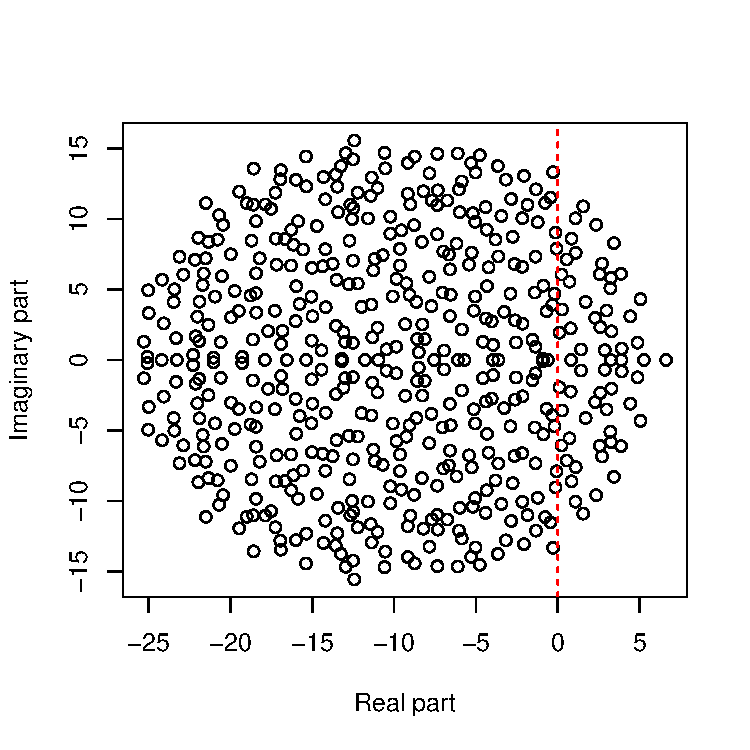
\includegraphics{bookdown-demo_files/figure-latex/unnamed-chunk-34-1.pdf}

\textbf{Extra reading: Elliptic raw}

In May's random matrix, the entries \(m_{ij}\), which represents the effect of species \(j\) on species \(i\)'s growth rate, are independently generated. However, in ecological networks, we usually model pairwise interaction such as consumer-resource, mutualism, and competition, in which cases, \(m_{ij}\) is not independent of \(m_{ji}\). For \textbf{consumer-resources interactions}, \(m_{ij}\) and \(m_{ji}\) are negatively correlated. For \textbf{mutualism or competition interaction}, \(m_{ij}\) and \(m_{ji}\) are positively correlated. Under the assumption that the pairwise interactions are correlated, we may show that the eigenvalues of the randomly generated Jacobian do not follow uniform distribution in a circle, but in an ellipse.

We build a function \texttt{BuildElliptic} with argument \(S\) is the number of species (i.e.~the dimension of the Jacobian), \(C\) is the connectance, \(d\) is the strength of self-limitation, \(\sigma\) is the variance (i.e.~the realized interaction strength) and \(\rho\) is the correlation of the pairwise interaction.

\begin{Shaded}
\begin{Highlighting}[]
\KeywordTok{library}\NormalTok{(ggplot2)}
\CommentTok{#### The function to build Elliptic law}
\NormalTok{BuildElliptic <-}\StringTok{ }\ControlFlowTok{function}\NormalTok{(S, C, d, sigma, rho)\{}
  
  \CommentTok{# sample coefficients in pairs}
\NormalTok{  pairs <-}\StringTok{ }\NormalTok{MASS}\OperatorTok{::}\KeywordTok{mvrnorm}\NormalTok{(}\DataTypeTok{n =}\NormalTok{ S }\OperatorTok{*}\StringTok{ }\NormalTok{(S}\DecValTok{-1}\NormalTok{) }\OperatorTok{/}\StringTok{ }\DecValTok{2}\NormalTok{,}
                         \DataTypeTok{mu =} \KeywordTok{c}\NormalTok{(}\DecValTok{0}\NormalTok{, }\DecValTok{0}\NormalTok{),}
                         \DataTypeTok{Sigma =}\NormalTok{ sigma}\OperatorTok{^}\DecValTok{2} \OperatorTok{*}\StringTok{ }\KeywordTok{matrix}\NormalTok{(}\KeywordTok{c}\NormalTok{(}\DecValTok{1}\NormalTok{, rho, rho, }\DecValTok{1}\NormalTok{), }\DecValTok{2}\NormalTok{, }\DecValTok{2}\NormalTok{))}
  
  \CommentTok{# build a completely filled matrix}
\NormalTok{  M <-}\StringTok{ }\KeywordTok{matrix}\NormalTok{(}\DecValTok{0}\NormalTok{, S, S)}
\NormalTok{  M[}\KeywordTok{upper.tri}\NormalTok{(M)] <-}\StringTok{ }\NormalTok{pairs[,}\DecValTok{1}\NormalTok{]}
\NormalTok{  M <-}\StringTok{ }\KeywordTok{t}\NormalTok{(M)}
\NormalTok{  M[}\KeywordTok{upper.tri}\NormalTok{(M)] <-}\StringTok{ }\NormalTok{pairs[,}\DecValTok{2}\NormalTok{]}
  
  \CommentTok{# determine which connections to retain (in pairs)}
\NormalTok{  Connections <-}\StringTok{ }\NormalTok{(}\KeywordTok{matrix}\NormalTok{(}\KeywordTok{runif}\NormalTok{(S }\OperatorTok{*}\StringTok{ }\NormalTok{S), S, S) }\OperatorTok{<=}\StringTok{ }\NormalTok{C) }\OperatorTok{*}\StringTok{ }\DecValTok{1} 
\NormalTok{  Connections[}\KeywordTok{lower.tri}\NormalTok{(Connections)] <-}\StringTok{ }\DecValTok{0}
  \KeywordTok{diag}\NormalTok{(Connections) <-}\StringTok{ }\DecValTok{0}
\NormalTok{  Connections <-}\StringTok{ }\NormalTok{Connections }\OperatorTok{+}\StringTok{ }\KeywordTok{t}\NormalTok{(Connections)}
\NormalTok{  M <-}\StringTok{ }\NormalTok{M }\OperatorTok{*}\StringTok{ }\NormalTok{Connections}
  
  \CommentTok{# set diagonals}
  \KeywordTok{diag}\NormalTok{(M) <-}\StringTok{ }\KeywordTok{diag}\NormalTok{(M) }\OperatorTok{-}\StringTok{ }\NormalTok{d}
  \KeywordTok{return}\NormalTok{(M)}
\NormalTok{\}}
\end{Highlighting}
\end{Shaded}

\begin{Shaded}
\begin{Highlighting}[]
\CommentTok{# consumer-resources interactions}
\NormalTok{M_CR <-}\StringTok{ }\KeywordTok{BuildElliptic}\NormalTok{(}\DataTypeTok{S =} \DecValTok{500}\NormalTok{, }\DataTypeTok{C =} \FloatTok{0.3}\NormalTok{, }\DataTypeTok{d =} \DecValTok{10}\NormalTok{, }\DataTypeTok{sigma =} \DecValTok{1}\NormalTok{, }\DataTypeTok{rho =} \FloatTok{-0.5}\NormalTok{)}
\NormalTok{EVals_CR <-}\StringTok{ }\KeywordTok{eigen}\NormalTok{(M_CR)}\OperatorTok{$}\NormalTok{values}
\NormalTok{Re.EVals_CR <-}\StringTok{ }\KeywordTok{Re}\NormalTok{(EVals_CR)}
\NormalTok{Im.EVals_CR <-}\StringTok{ }\KeywordTok{Im}\NormalTok{(EVals_CR)}

\CommentTok{# mutualism or competition}
\NormalTok{M_MC <-}\StringTok{ }\KeywordTok{BuildElliptic}\NormalTok{(}\DataTypeTok{S =} \DecValTok{500}\NormalTok{, }\DataTypeTok{C =} \FloatTok{0.3}\NormalTok{, }\DataTypeTok{d =} \DecValTok{10}\NormalTok{, }\DataTypeTok{sigma =} \DecValTok{1}\NormalTok{, }\DataTypeTok{rho =} \FloatTok{0.5}\NormalTok{)}
\NormalTok{EVals_MC <-}\StringTok{ }\KeywordTok{eigen}\NormalTok{(M_MC)}\OperatorTok{$}\NormalTok{values}
\NormalTok{Re.EVals_MC <-}\StringTok{ }\KeywordTok{Re}\NormalTok{(EVals_MC)}
\NormalTok{Im.EVals_MC <-}\StringTok{ }\KeywordTok{Im}\NormalTok{(EVals_MC)}

\CommentTok{# combine data}
\NormalTok{Re.EVals <-}\StringTok{ }\KeywordTok{c}\NormalTok{(Re.EVals_CR, Re.EVals_MC)}
\NormalTok{Im.EVals <-}\StringTok{ }\KeywordTok{c}\NormalTok{(Im.EVals_CR, Im.EVals_MC)}

\CommentTok{# visualization}
\KeywordTok{plot}\NormalTok{(Re.EVals, Im.EVals, }\DataTypeTok{xlab =} \StringTok{"Real part"}\NormalTok{, }\DataTypeTok{ylab =} \StringTok{"Imaginary part"}\NormalTok{, }\DataTypeTok{type =} \StringTok{"n"}\NormalTok{)}
\KeywordTok{points}\NormalTok{(Re.EVals_CR, Im.EVals_CR, }\DataTypeTok{col =} \StringTok{"green"}\NormalTok{)}
\KeywordTok{points}\NormalTok{(Re.EVals_MC, Im.EVals_MC, }\DataTypeTok{col =} \StringTok{"blue"}\NormalTok{)}
\KeywordTok{abline}\NormalTok{(}\DataTypeTok{v =} \DecValTok{0}\NormalTok{, }\DataTypeTok{col =} \StringTok{"red"}\NormalTok{, }\DataTypeTok{lty =} \DecValTok{2}\NormalTok{)}
\KeywordTok{legend}\NormalTok{(}\StringTok{"topleft"}\NormalTok{, }\DataTypeTok{legend =} \KeywordTok{c}\NormalTok{(}\StringTok{"Resource-consumer"}\NormalTok{, }\StringTok{"Mutualism or Competition"}\NormalTok{), }\DataTypeTok{col =} \KeywordTok{c}\NormalTok{(}\StringTok{"green"}\NormalTok{, }\StringTok{"blue"}\NormalTok{), }\DataTypeTok{pch =} \DecValTok{1}\NormalTok{)}
\end{Highlighting}
\end{Shaded}

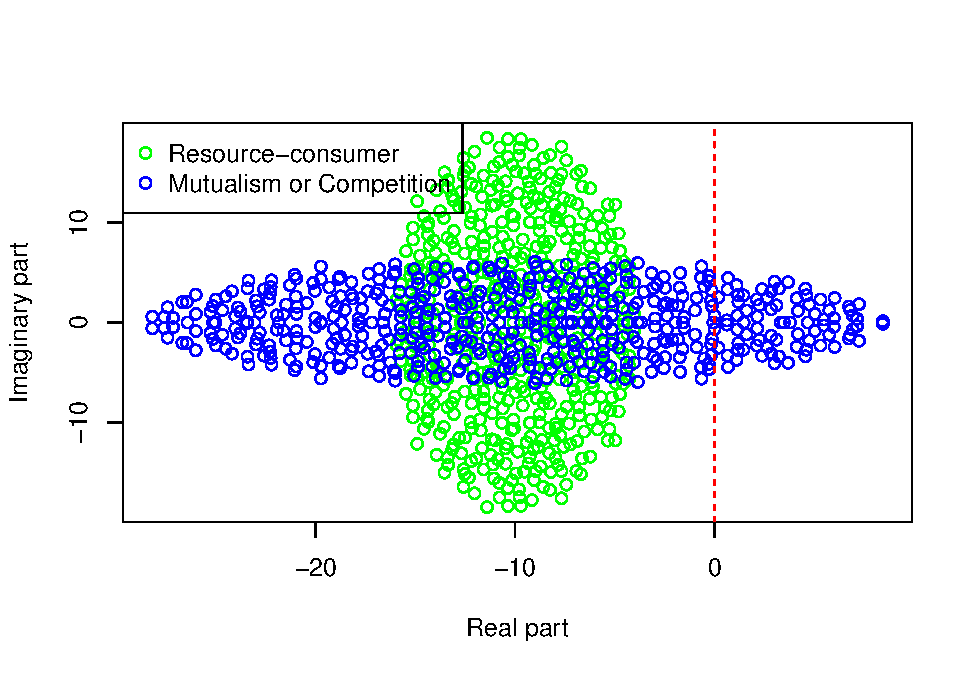
\includegraphics{bookdown-demo_files/figure-latex/unnamed-chunk-36-1.pdf}

\hypertarget{week-13---parameter-space-for-apparent-competition-model}{%
\chapter*{Week 13 - Parameter space for apparent competition model}\label{week-13---parameter-space-for-apparent-competition-model}}
\addcontentsline{toc}{chapter}{Week 13 - Parameter space for apparent competition model}

Here, we are going to visualize the outcomes of apparent competition in the \(r_1/a_1\) -- \(r_2/a_2\) space:
\begin{align*}
\frac{dN_1}{dt} &= r_1N_1(1-\frac{N_1}{K_1}) - a_1N_1P\\
\frac{dN_2}{dt} &= r_2N_2(1-\frac{N_2}{K_2}) - a_2N_2P\\
\frac{dP}{dt} &= e_1a_1N_1P + e_2a_2N_2P - mP.
\end{align*}
Two prey \(N_1\) and \(N_2\) grow logistically with intrinsic growth rate \(r_1\) and \(r_2\) and carrying capacity \(K_1\) and \(K_2\). Predator \(P\) consumes two prey following Holling type I functional response, with \(a_1\) and \(a_2\) representing the consumption rate of \(N_1\) and \(N_2\) by predator respectively. After consumption, the assimilation rate are \(e_1\) and \(e_2\). The death rate of predator is represented by \(m\).

\begin{Shaded}
\begin{Highlighting}[]
\KeywordTok{library}\NormalTok{(deSolve)}
\KeywordTok{library}\NormalTok{(ggplot2)}
\CommentTok{#### Create a function to evaluate the competition outcome}
\NormalTok{Apparent_logistic_func <-}\StringTok{ }\ControlFlowTok{function}\NormalTok{(r1, r2, other.parameters)\{}

  \CommentTok{# specify the model}
\NormalTok{  Apparent_logistic_model <-}\StringTok{ }\ControlFlowTok{function}\NormalTok{(times, state, parms) \{}
    \KeywordTok{with}\NormalTok{(}\KeywordTok{as.list}\NormalTok{(}\KeywordTok{c}\NormalTok{(state, parms)), \{}
\NormalTok{      dN1_dt =}\StringTok{ }\NormalTok{r1 }\OperatorTok{*}\StringTok{ }\NormalTok{N1 }\OperatorTok{*}\StringTok{ }\NormalTok{(}\DecValTok{1} \OperatorTok{-}\StringTok{ }\NormalTok{N1 }\OperatorTok{/}\StringTok{ }\NormalTok{K1) }\OperatorTok{-}\StringTok{ }\NormalTok{a1 }\OperatorTok{*}\StringTok{ }\NormalTok{N1 }\OperatorTok{*}\StringTok{ }\NormalTok{P}
\NormalTok{      dN2_dt =}\StringTok{ }\NormalTok{r2 }\OperatorTok{*}\StringTok{ }\NormalTok{N2 }\OperatorTok{*}\StringTok{ }\NormalTok{(}\DecValTok{1} \OperatorTok{-}\StringTok{ }\NormalTok{N2 }\OperatorTok{/}\StringTok{ }\NormalTok{K2) }\OperatorTok{-}\StringTok{ }\NormalTok{a2 }\OperatorTok{*}\StringTok{ }\NormalTok{N2 }\OperatorTok{*}\StringTok{ }\NormalTok{P}
\NormalTok{      dP_dt =}\StringTok{ }\NormalTok{e1 }\OperatorTok{*}\StringTok{ }\NormalTok{a1 }\OperatorTok{*}\StringTok{ }\NormalTok{N1 }\OperatorTok{*}\StringTok{ }\NormalTok{P }\OperatorTok{+}\StringTok{ }\NormalTok{e2 }\OperatorTok{*}\StringTok{ }\NormalTok{a2 }\OperatorTok{*}\StringTok{ }\NormalTok{N2 }\OperatorTok{*}\StringTok{ }\NormalTok{P }\OperatorTok{-}\StringTok{ }\NormalTok{d }\OperatorTok{*}\StringTok{ }\NormalTok{P}
      \KeywordTok{return}\NormalTok{(}\KeywordTok{list}\NormalTok{(}\KeywordTok{c}\NormalTok{(dN1_dt, dN2_dt, dP_dt)))}
\NormalTok{    \})}
\NormalTok{  \}}

  \CommentTok{# model parameters}
\NormalTok{  times <-}\StringTok{ }\KeywordTok{seq}\NormalTok{(}\DecValTok{0}\NormalTok{, }\DecValTok{3000}\NormalTok{, }\DataTypeTok{by =} \DecValTok{10}\NormalTok{)}
\NormalTok{  state <-}\StringTok{ }\KeywordTok{c}\NormalTok{(}\DataTypeTok{N1 =} \FloatTok{0.1}\NormalTok{, }\DataTypeTok{N2 =} \FloatTok{0.1}\NormalTok{, }\DataTypeTok{P =} \DecValTok{1}\NormalTok{)}
\NormalTok{  parms <-}\StringTok{ }\KeywordTok{c}\NormalTok{(}\DataTypeTok{r1 =}\NormalTok{ r1, }\DataTypeTok{r2 =}\NormalTok{ r2, other.parameters)}

  \CommentTok{# run the ode}
\NormalTok{  pop_size <-}\StringTok{ }\KeywordTok{ode}\NormalTok{(}\DataTypeTok{func =}\NormalTok{ Apparent_logistic_model, }\DataTypeTok{times =}\NormalTok{ times, }\DataTypeTok{y =}\NormalTok{ state, }\DataTypeTok{parms =}\NormalTok{ parms)}

  \CommentTok{# return final population size}
\NormalTok{  N_final <-}\StringTok{ }\KeywordTok{nrow}\NormalTok{(}\KeywordTok{na.omit}\NormalTok{(pop_size))   }\CommentTok{# remove NAN's}
  \KeywordTok{return}\NormalTok{(pop_size[N_final, }\DecValTok{-1}\NormalTok{])}

\NormalTok{\}}


\CommentTok{#### Set up parameter space of interest}
\NormalTok{Parms <-}\StringTok{ }\KeywordTok{c}\NormalTok{(}\DataTypeTok{r1 =} \FloatTok{0.1}\NormalTok{, }\DataTypeTok{r2 =} \FloatTok{0.1}\NormalTok{, }\DataTypeTok{a1 =} \FloatTok{0.35}\NormalTok{, }\DataTypeTok{a2 =} \FloatTok{0.35}\NormalTok{, }\DataTypeTok{e1 =} \FloatTok{0.4}\NormalTok{, }\DataTypeTok{e2 =} \FloatTok{0.5}\NormalTok{, }\DataTypeTok{d =} \FloatTok{0.8}\NormalTok{, }\DataTypeTok{K1 =} \DecValTok{15}\NormalTok{, }\DataTypeTok{K2 =} \DecValTok{12}\NormalTok{)}
\NormalTok{r_min <-}\StringTok{ }\FloatTok{0.1}
\NormalTok{r_max <-}\StringTok{ }\FloatTok{0.7}
\NormalTok{n <-}\StringTok{ }\DecValTok{100}
\NormalTok{r1.vec <-}\StringTok{ }\KeywordTok{seq}\NormalTok{(r_min, r_max, }\DataTypeTok{length.out =}\NormalTok{ n)}
\NormalTok{r2.vec <-}\StringTok{ }\KeywordTok{seq}\NormalTok{(r_min, r_max, }\DataTypeTok{length.out =}\NormalTok{ n)}


\CommentTok{#### Create parameter space and saving space}
\NormalTok{comp_out <-}\StringTok{ }\KeywordTok{expand.grid}\NormalTok{(}\DataTypeTok{r1 =}\NormalTok{ r1.vec, }\DataTypeTok{r2 =}\NormalTok{ r2.vec)}
\NormalTok{comp_out <-}\StringTok{ }\KeywordTok{as.data.frame}\NormalTok{(}\KeywordTok{cbind}\NormalTok{(comp_out,}
                                \KeywordTok{matrix}\NormalTok{(}\DecValTok{0}\NormalTok{, }\DataTypeTok{nrow =} \KeywordTok{dim}\NormalTok{(comp_out)[}\DecValTok{1}\NormalTok{], }\DataTypeTok{ncol =} \DecValTok{3}\NormalTok{)))}
\KeywordTok{head}\NormalTok{(comp_out)}
\end{Highlighting}
\end{Shaded}

\begin{verbatim}
##          r1  r2 1 2 3
## 1 0.1000000 0.1 0 0 0
## 2 0.1060606 0.1 0 0 0
## 3 0.1121212 0.1 0 0 0
## 4 0.1181818 0.1 0 0 0
## 5 0.1242424 0.1 0 0 0
## 6 0.1303030 0.1 0 0 0
\end{verbatim}

\begin{Shaded}
\begin{Highlighting}[]
\CommentTok{#### Apply the function across the parameter space}
\NormalTok{start_time <-}\StringTok{ }\KeywordTok{Sys.time}\NormalTok{() }\CommentTok{# starting time}
\ControlFlowTok{for}\NormalTok{(i }\ControlFlowTok{in} \DecValTok{1}\OperatorTok{:}\KeywordTok{dim}\NormalTok{(comp_out)[}\DecValTok{1}\NormalTok{])\{}
\NormalTok{  comp_out[i, }\DecValTok{3}\OperatorTok{:}\DecValTok{5}\NormalTok{] <-}\StringTok{ }\KeywordTok{Apparent_logistic_func}\NormalTok{(}\DataTypeTok{r1 =}\NormalTok{ comp_out}\OperatorTok{$}\NormalTok{r1[i],}
                                             \DataTypeTok{r2 =}\NormalTok{ comp_out}\OperatorTok{$}\NormalTok{r2[i],}
                                             \DataTypeTok{other.parameters =}\NormalTok{ Parms[}\OperatorTok{-}\KeywordTok{c}\NormalTok{(}\DecValTok{1}\OperatorTok{:}\DecValTok{2}\NormalTok{)])}
\NormalTok{\}}
\NormalTok{end_time <-}\StringTok{ }\KeywordTok{Sys.time}\NormalTok{() }\CommentTok{# ending time}
\NormalTok{end_time }\OperatorTok{-}\StringTok{ }\NormalTok{start_time }\CommentTok{# total time spent}
\end{Highlighting}
\end{Shaded}

\begin{verbatim}
## Time difference of 7.798916 mins
\end{verbatim}

\begin{Shaded}
\begin{Highlighting}[]
\CommentTok{#### Determine outcome status}
\NormalTok{comp_out}\OperatorTok{$}\NormalTok{Outcome <-}
\StringTok{  }\KeywordTok{ifelse}\NormalTok{ (comp_out[, }\DecValTok{3}\NormalTok{] }\OperatorTok{<}\StringTok{ }\FloatTok{1e-4}\NormalTok{, }\StringTok{"N2 win"}\NormalTok{,}
          \KeywordTok{ifelse}\NormalTok{(comp_out[, }\DecValTok{4}\NormalTok{] }\OperatorTok{<}\StringTok{ }\FloatTok{1e-4}\NormalTok{, }\StringTok{"N1 win"}\NormalTok{, }\StringTok{"Coexist"}\NormalTok{))}
\end{Highlighting}
\end{Shaded}

\begin{Shaded}
\begin{Highlighting}[]
\CommentTok{#### Visualize the competition outcomes in the grids -- base R}
\NormalTok{x <-}\StringTok{ }\NormalTok{comp_out}\OperatorTok{$}\NormalTok{r1 }\OperatorTok{/}\StringTok{ }\NormalTok{Parms[}\DecValTok{3}\NormalTok{]}
\NormalTok{y <-}\StringTok{ }\NormalTok{comp_out}\OperatorTok{$}\NormalTok{r2 }\OperatorTok{/}\StringTok{ }\NormalTok{Parms[}\DecValTok{4}\NormalTok{]}
\NormalTok{z <-}\StringTok{ }\KeywordTok{as.factor}\NormalTok{(comp_out}\OperatorTok{$}\NormalTok{Outcome) }\CommentTok{# Levels: Coexist N1 win N2 win}
\NormalTok{color <-}\StringTok{ }\KeywordTok{c}\NormalTok{(}\StringTok{"red"}\NormalTok{, }\StringTok{"blue"}\NormalTok{, }\StringTok{"green"}\NormalTok{)}
\KeywordTok{plot}\NormalTok{(x, y, }\DataTypeTok{type =} \StringTok{"n"}\NormalTok{, }\DataTypeTok{xlab =} \StringTok{"r1/a1"}\NormalTok{, }\DataTypeTok{ylab =} \StringTok{"r2/a2"}\NormalTok{)}
\NormalTok{size <-}\StringTok{ }\FloatTok{0.008571429} \CommentTok{#0.003/0.35}
\ControlFlowTok{for}\NormalTok{(i }\ControlFlowTok{in} \DecValTok{1}\OperatorTok{:}\KeywordTok{length}\NormalTok{(z))\{}
  \KeywordTok{rect}\NormalTok{(x[i] }\OperatorTok{-}\StringTok{ }\NormalTok{size, y[i] }\OperatorTok{-}\StringTok{ }\NormalTok{size, x[i] }\OperatorTok{+}\StringTok{ }\NormalTok{size, y[i] }\OperatorTok{+}\StringTok{ }\NormalTok{size, }\DataTypeTok{col =}\NormalTok{ color[z[i]], }\DataTypeTok{border =}\NormalTok{ color[z[i]])}
\NormalTok{\}}
\KeywordTok{abline}\NormalTok{(}\DataTypeTok{a =} \DecValTok{0}\NormalTok{, }\DataTypeTok{b =}\NormalTok{ (}\DecValTok{1} \OperatorTok{-}\StringTok{ }\NormalTok{Parms[}\DecValTok{7}\NormalTok{] }\OperatorTok{/}\StringTok{ }\NormalTok{(Parms[}\DecValTok{5}\NormalTok{] }\OperatorTok{*}\StringTok{ }\NormalTok{Parms[}\DecValTok{3}\NormalTok{] }\OperatorTok{*}\StringTok{ }\NormalTok{Parms[}\DecValTok{8}\NormalTok{])), }\DataTypeTok{lwd =} \DecValTok{4}\NormalTok{)}
\KeywordTok{abline}\NormalTok{(}\DataTypeTok{a =} \DecValTok{0}\NormalTok{, }\DataTypeTok{b =}\NormalTok{ (}\DecValTok{1} \OperatorTok{-}\StringTok{ }\NormalTok{Parms[}\DecValTok{7}\NormalTok{] }\OperatorTok{/}\StringTok{ }\NormalTok{(Parms[}\DecValTok{6}\NormalTok{] }\OperatorTok{*}\StringTok{ }\NormalTok{Parms[}\DecValTok{4}\NormalTok{] }\OperatorTok{*}\StringTok{ }\NormalTok{Parms[}\DecValTok{9}\NormalTok{]))}\OperatorTok{^-}\DecValTok{1}\NormalTok{,, }\DataTypeTok{lwd =} \DecValTok{4}\NormalTok{)}
\KeywordTok{text}\NormalTok{(}\FloatTok{0.5}\NormalTok{, }\FloatTok{1.5}\NormalTok{, }\DataTypeTok{labels =} \StringTok{"N2 wins"}\NormalTok{)}
\KeywordTok{text}\NormalTok{(}\FloatTok{1.5}\NormalTok{, }\FloatTok{0.5}\NormalTok{, }\DataTypeTok{labels =} \StringTok{"N1 wins"}\NormalTok{)}
\KeywordTok{text}\NormalTok{(}\FloatTok{1.5}\NormalTok{, }\FloatTok{1.5}\NormalTok{, }\DataTypeTok{labels =} \StringTok{"Coexist"}\NormalTok{)}
\end{Highlighting}
\end{Shaded}

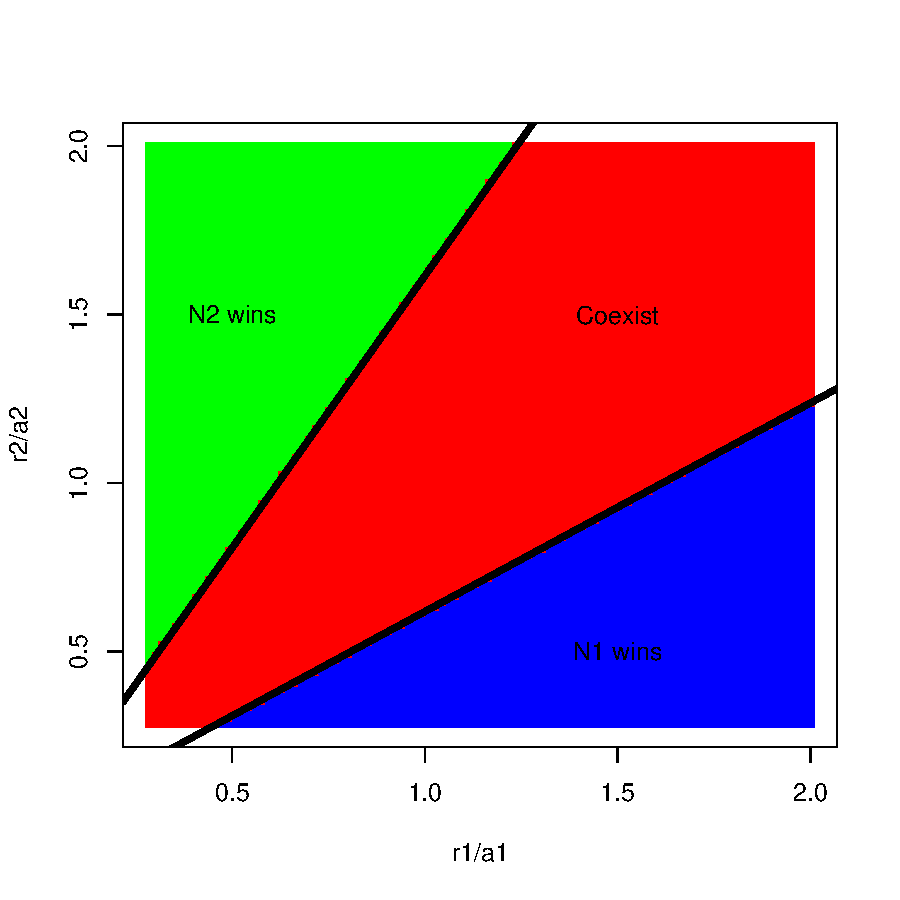
\includegraphics{bookdown-demo_files/figure-latex/unnamed-chunk-38-1.pdf}

\begin{Shaded}
\begin{Highlighting}[]
\CommentTok{#### Visualize the competition outcomes in the grids -- ggplot}
\KeywordTok{ggplot}\NormalTok{(comp_out, }\KeywordTok{aes}\NormalTok{(}\DataTypeTok{x =}\NormalTok{ r1}\OperatorTok{/}\NormalTok{Parms[}\DecValTok{3}\NormalTok{], }\DataTypeTok{y =}\NormalTok{ r2}\OperatorTok{/}\NormalTok{Parms[}\DecValTok{4}\NormalTok{], }\DataTypeTok{z =}\NormalTok{ Outcome, }\DataTypeTok{fill =}\NormalTok{ Outcome)) }\OperatorTok{+}
\StringTok{  }\KeywordTok{geom_tile}\NormalTok{() }\OperatorTok{+}
\StringTok{  }\KeywordTok{geom_abline}\NormalTok{(}\DataTypeTok{intercept =} \DecValTok{0}\NormalTok{, }\DataTypeTok{slope =}\NormalTok{ (}\DecValTok{1} \OperatorTok{-}\StringTok{ }\NormalTok{Parms[}\DecValTok{7}\NormalTok{] }\OperatorTok{/}\StringTok{ }\NormalTok{(Parms[}\DecValTok{5}\NormalTok{] }\OperatorTok{*}\StringTok{ }\NormalTok{Parms[}\DecValTok{3}\NormalTok{] }\OperatorTok{*}\StringTok{ }\NormalTok{Parms[}\DecValTok{8}\NormalTok{])), }\DataTypeTok{size =} \FloatTok{1.5}\NormalTok{) }\OperatorTok{+}
\StringTok{  }\KeywordTok{geom_abline}\NormalTok{(}\DataTypeTok{intercept =} \DecValTok{0}\NormalTok{, }\DataTypeTok{slope =}\NormalTok{ (}\DecValTok{1} \OperatorTok{-}\StringTok{ }\NormalTok{Parms[}\DecValTok{7}\NormalTok{] }\OperatorTok{/}\StringTok{ }\NormalTok{(Parms[}\DecValTok{6}\NormalTok{] }\OperatorTok{*}\StringTok{ }\NormalTok{Parms[}\DecValTok{4}\NormalTok{] }\OperatorTok{*}\StringTok{ }\NormalTok{Parms[}\DecValTok{9}\NormalTok{]))}\OperatorTok{^-}\DecValTok{1}\NormalTok{, }\DataTypeTok{size =} \FloatTok{1.5}\NormalTok{) }\OperatorTok{+}
\StringTok{  }\KeywordTok{labs}\NormalTok{(}\DataTypeTok{x =} \KeywordTok{expression}\NormalTok{(r[}\DecValTok{1}\NormalTok{]}\OperatorTok{/}\NormalTok{a[}\DecValTok{1}\NormalTok{]), }\DataTypeTok{y =} \KeywordTok{expression}\NormalTok{(r[}\DecValTok{2}\NormalTok{]}\OperatorTok{/}\NormalTok{a[}\DecValTok{2}\NormalTok{])) }\OperatorTok{+}
\StringTok{  }\KeywordTok{scale_x_continuous}\NormalTok{(}\DataTypeTok{limits =} \KeywordTok{c}\NormalTok{(r_min}\OperatorTok{/}\NormalTok{Parms[}\DecValTok{3}\NormalTok{], r_max}\OperatorTok{/}\NormalTok{Parms[}\DecValTok{4}\NormalTok{]), }\DataTypeTok{expand =} \KeywordTok{c}\NormalTok{(}\DecValTok{0}\NormalTok{, }\DecValTok{0}\NormalTok{)) }\OperatorTok{+}
\StringTok{  }\KeywordTok{scale_y_continuous}\NormalTok{(}\DataTypeTok{limits =} \KeywordTok{c}\NormalTok{(r_min}\OperatorTok{/}\NormalTok{Parms[}\DecValTok{3}\NormalTok{], r_max}\OperatorTok{/}\NormalTok{Parms[}\DecValTok{4}\NormalTok{]), }\DataTypeTok{expand =} \KeywordTok{c}\NormalTok{(}\DecValTok{0}\NormalTok{, }\DecValTok{0}\NormalTok{)) }\OperatorTok{+}
\StringTok{  }\KeywordTok{scale_fill_brewer}\NormalTok{(}\DataTypeTok{palette =} \StringTok{"Set1"}\NormalTok{) }\OperatorTok{+}
\StringTok{  }\KeywordTok{theme_bw}\NormalTok{(}\DataTypeTok{base_size =} \DecValTok{14}\NormalTok{) }\OperatorTok{+}
\StringTok{  }\KeywordTok{theme}\NormalTok{(}\DataTypeTok{panel.grid =} \KeywordTok{element_blank}\NormalTok{()) }\OperatorTok{+}
\StringTok{  }\KeywordTok{coord_fixed}\NormalTok{(}\DataTypeTok{ratio =} \DecValTok{1}\NormalTok{) }\OperatorTok{+}
\StringTok{  }\KeywordTok{annotate}\NormalTok{(}\DataTypeTok{geom =} \StringTok{"text"}\NormalTok{, }\DataTypeTok{x =} \FloatTok{0.5}\NormalTok{, }\DataTypeTok{y =} \FloatTok{1.5}\NormalTok{, }\DataTypeTok{label =} \StringTok{"bold(bolditalic(N[2])~wins)"}\NormalTok{, }\DataTypeTok{parse =}\NormalTok{ T) }\OperatorTok{+}
\StringTok{  }\KeywordTok{annotate}\NormalTok{(}\DataTypeTok{geom =} \StringTok{"text"}\NormalTok{, }\DataTypeTok{x =} \FloatTok{1.5}\NormalTok{, }\DataTypeTok{y =} \FloatTok{1.5}\NormalTok{, }\DataTypeTok{label =} \StringTok{"bold(Coexist)"}\NormalTok{, }\DataTypeTok{parse =}\NormalTok{ T) }\OperatorTok{+}
\StringTok{  }\KeywordTok{annotate}\NormalTok{(}\DataTypeTok{geom =} \StringTok{"text"}\NormalTok{, }\DataTypeTok{x =} \FloatTok{1.5}\NormalTok{, }\DataTypeTok{y =} \FloatTok{0.5}\NormalTok{, }\DataTypeTok{label =} \StringTok{"bold(bolditalic(N[1])~wins)"}\NormalTok{, }\DataTypeTok{parse =}\NormalTok{ T)}
\end{Highlighting}
\end{Shaded}

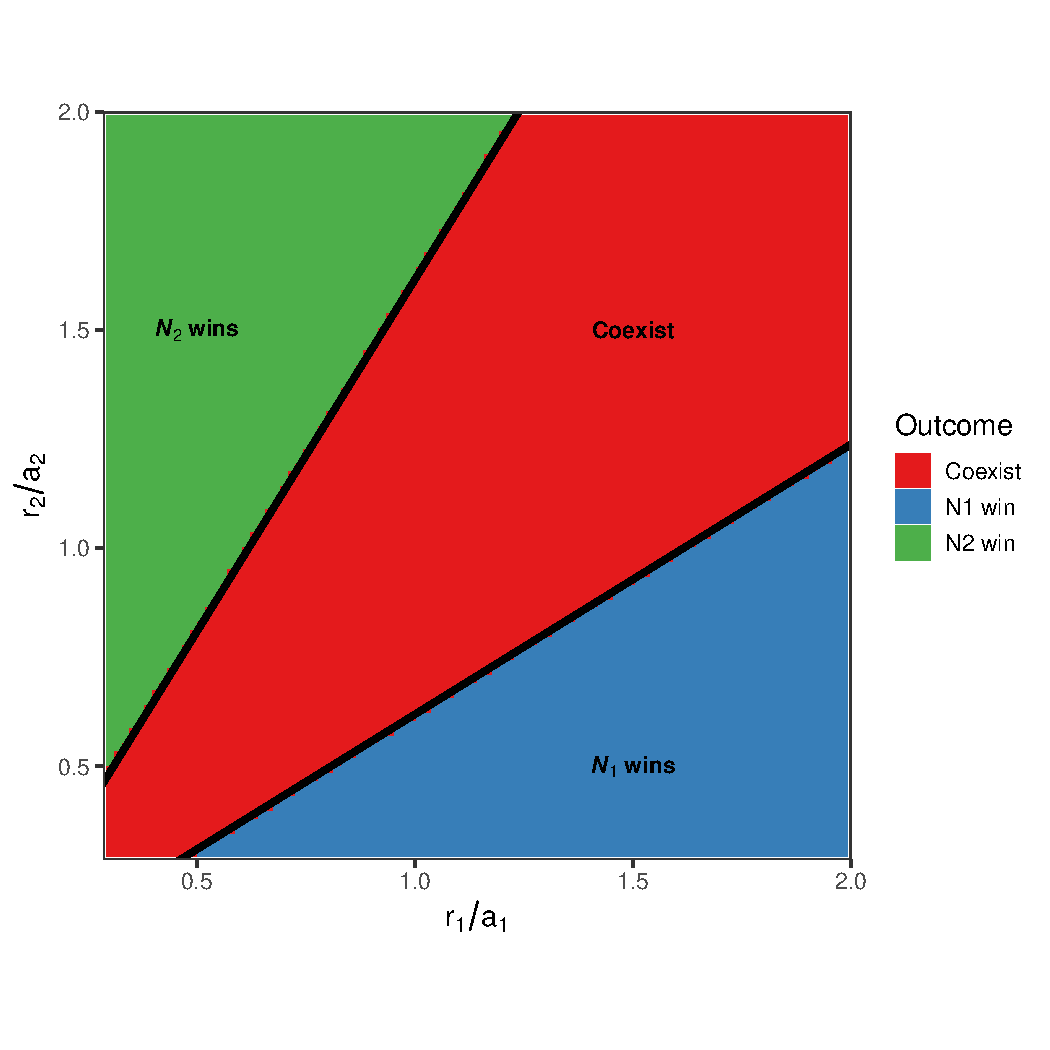
\includegraphics{bookdown-demo_files/figure-latex/unnamed-chunk-39-1.pdf}

If the parameter space is extended and sliced into more tiny grid, the outcomes will be more complete:
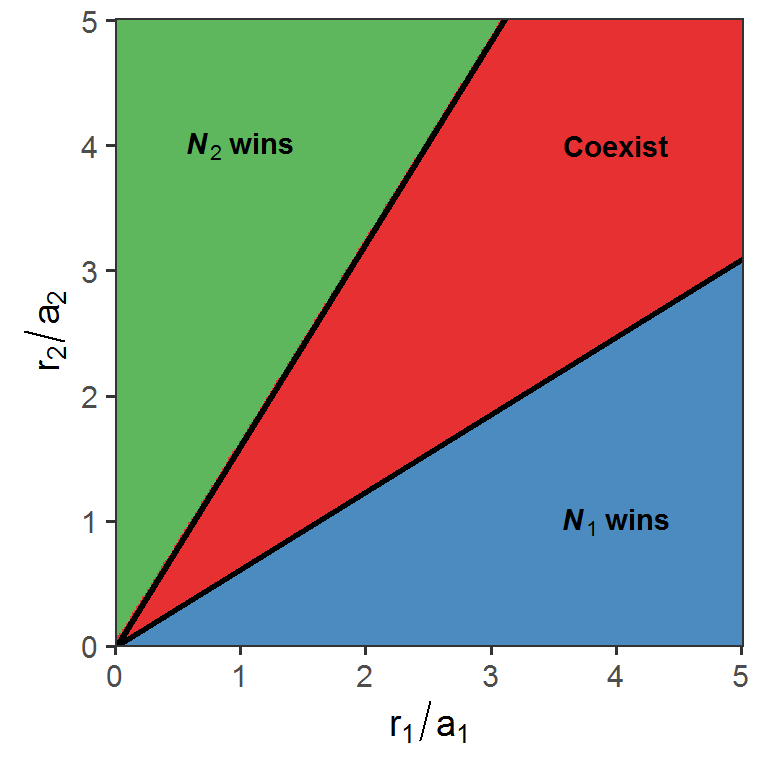
\includegraphics{assignment_figures/W13.png}

\hypertarget{week-14---resource-competition}{%
\chapter*{Week 14 - Resource competition}\label{week-14---resource-competition}}
\addcontentsline{toc}{chapter}{Week 14 - Resource competition}

\textbf{Part 1 - R* rule}

In this part of the lab section, we are going to analyze the consumer-resource dynamics with two consumers and one resource:
\begin{align*}
\frac {dN_{1}}{dt} &= e_{1}a_{1}RN_{1}-dN_{1}\\
\frac {dN_{2}}{dt} &= e_{2}a_{2}RN_{2}-dN_{2}\\
\frac {dR}{dt} &= d(S_{0}-R)-a_{1}RN_{1}-a_{2}RN_{2}\\
\end{align*}

Please simulate the model using the parameter set (\(N_{1(0)}\) = 2, \(N_{2(0)}\) = 2, \(R\) = 0.1, \(a_1\) = 0.4, \(a_2\) = 0.6, \(e_1\) = 1, \(e_2\) = 1, \(d\) = 0.01, \(S_0\) = 0.1) and visualize the population trajectories of the two consumers as well as the resource.

Below is a plot of resource level vs.~consumers' per capita growth rate. What would you predict about the system dynamics?

\begin{Shaded}
\begin{Highlighting}[]
\KeywordTok{library}\NormalTok{(tidyverse)}
\KeywordTok{library}\NormalTok{(deSolve)}

\CommentTok{### Parameters}
\NormalTok{a1 <-}\StringTok{ }\FloatTok{0.4} 
\NormalTok{a2 <-}\StringTok{ }\FloatTok{0.6}
\NormalTok{e1 <-}\StringTok{ }\DecValTok{1}
\NormalTok{e2 <-}\StringTok{ }\DecValTok{1}
\NormalTok{d <-}\StringTok{ }\FloatTok{0.01} 
\NormalTok{S0 <-}\StringTok{ }\FloatTok{0.1}

\CommentTok{### Resource level vs. consumers' per capita population growth}
\KeywordTok{data.frame}\NormalTok{(}\DataTypeTok{R =} \KeywordTok{seq}\NormalTok{(}\DecValTok{0}\NormalTok{, }\FloatTok{0.1}\NormalTok{, }\FloatTok{0.001}\NormalTok{)) }\OperatorTok
\StringTok{  }\KeywordTok{mutate}\NormalTok{(}\DataTypeTok{N1 =}\NormalTok{ e1}\OperatorTok{*}\NormalTok{a1}\OperatorTok{*}\NormalTok{R}\OperatorTok{-}\NormalTok{d,}
         \DataTypeTok{N2 =}\NormalTok{ e2}\OperatorTok{*}\NormalTok{a2}\OperatorTok{*}\NormalTok{R}\OperatorTok{-}\NormalTok{d) }\OperatorTok
\StringTok{  }\KeywordTok{gather}\NormalTok{(}\DataTypeTok{key =} \StringTok{"Species"}\NormalTok{, }\DataTypeTok{value =} \StringTok{"Growth"}\NormalTok{, N1}\OperatorTok{:}\NormalTok{N2) }\OperatorTok
\StringTok{  }\KeywordTok{ggplot}\NormalTok{(}\KeywordTok{aes}\NormalTok{(}\DataTypeTok{x =}\NormalTok{ R, }\DataTypeTok{y =}\NormalTok{ Growth, }\DataTypeTok{color =}\NormalTok{ Species)) }\OperatorTok{+}
\StringTok{  }\KeywordTok{geom_line}\NormalTok{() }\OperatorTok{+}\StringTok{ }
\StringTok{  }\KeywordTok{geom_hline}\NormalTok{(}\DataTypeTok{yintercept =} \DecValTok{0}\NormalTok{, }\DataTypeTok{linetype =} \StringTok{"dashed"}\NormalTok{) }\OperatorTok{+}\StringTok{ }
\StringTok{  }\KeywordTok{labs}\NormalTok{(}\DataTypeTok{x =} \StringTok{"Resource level"}\NormalTok{, }\DataTypeTok{y =} \StringTok{"Per capita growth rate"}\NormalTok{) }\OperatorTok{+}
\StringTok{  }\KeywordTok{theme_classic}\NormalTok{(}\DataTypeTok{base_size =} \DecValTok{14}\NormalTok{)}
\end{Highlighting}
\end{Shaded}

\begin{center}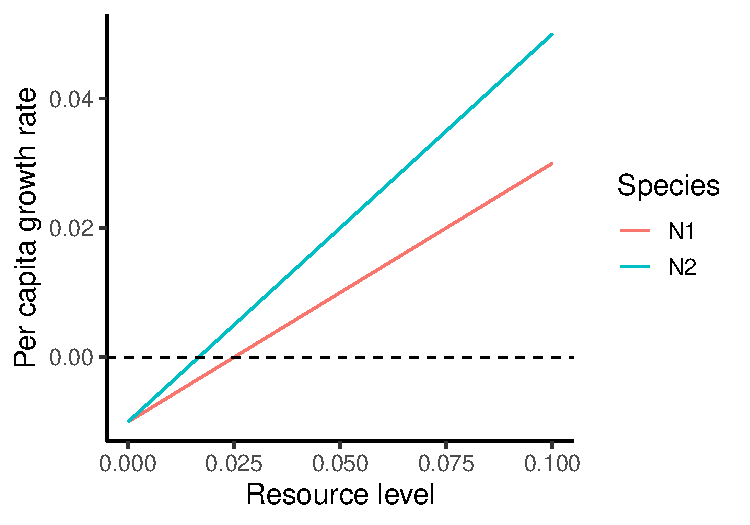
\includegraphics[width=0.7\linewidth]{bookdown-demo_files/figure-latex/unnamed-chunk-41-1} \end{center}

\begin{Shaded}
\begin{Highlighting}[]
\CommentTok{### Model specification}
\NormalTok{CR_model_2C_1R <-}\StringTok{ }\ControlFlowTok{function}\NormalTok{(times, state, parms)\{}
  \KeywordTok{with}\NormalTok{(}\KeywordTok{as.list}\NormalTok{(}\KeywordTok{c}\NormalTok{(state, parms)), \{}
\NormalTok{    dN1_dt =}\StringTok{ }\NormalTok{e1}\OperatorTok{*}\NormalTok{a1}\OperatorTok{*}\NormalTok{R}\OperatorTok{*}\NormalTok{N1 }\OperatorTok{-}\StringTok{ }\NormalTok{d}\OperatorTok{*}\NormalTok{N1}
\NormalTok{    dN2_dt =}\StringTok{ }\NormalTok{e2}\OperatorTok{*}\NormalTok{a2}\OperatorTok{*}\NormalTok{R}\OperatorTok{*}\NormalTok{N2 }\OperatorTok{-}\StringTok{ }\NormalTok{d}\OperatorTok{*}\NormalTok{N2}
\NormalTok{    dR_dt =}\StringTok{  }\NormalTok{d}\OperatorTok{*}\NormalTok{(S0}\OperatorTok{-}\NormalTok{R) }\OperatorTok{-}\StringTok{ }\NormalTok{a1}\OperatorTok{*}\NormalTok{R}\OperatorTok{*}\NormalTok{N1 }\OperatorTok{-}\StringTok{ }\NormalTok{a2}\OperatorTok{*}\NormalTok{R}\OperatorTok{*}\NormalTok{N2}
    \KeywordTok{return}\NormalTok{(}\KeywordTok{list}\NormalTok{(}\KeywordTok{c}\NormalTok{(dN1_dt, dN2_dt, dR_dt)))}
\NormalTok{  \})}
\NormalTok{\}}

\CommentTok{### Model parameters}
\NormalTok{times <-}\StringTok{ }\KeywordTok{seq}\NormalTok{(}\FloatTok{0.1}\NormalTok{, }\DecValTok{1000}\NormalTok{, }\DataTypeTok{by =} \FloatTok{0.1}\NormalTok{)  }
\NormalTok{state <-}\StringTok{ }\KeywordTok{c}\NormalTok{(}\DataTypeTok{N1 =} \DecValTok{2}\NormalTok{, }\DataTypeTok{N2 =} \DecValTok{2}\NormalTok{, }\DataTypeTok{R =} \FloatTok{0.1}\NormalTok{)  }
\NormalTok{parms <-}\StringTok{ }\KeywordTok{c}\NormalTok{(}\DataTypeTok{a1 =} \FloatTok{0.4}\NormalTok{, }\DataTypeTok{a2 =} \FloatTok{0.6}\NormalTok{, }\DataTypeTok{e1 =} \DecValTok{1}\NormalTok{, }\DataTypeTok{e2 =} \DecValTok{1}\NormalTok{, }\DataTypeTok{d =} \FloatTok{0.01}\NormalTok{, }\DataTypeTok{S0 =} \FloatTok{0.1}\NormalTok{)}

\CommentTok{### Model application}
\NormalTok{pop_size <-}\StringTok{ }\KeywordTok{ode}\NormalTok{(}\DataTypeTok{func =}\NormalTok{ CR_model_2C_1R, }\DataTypeTok{times =}\NormalTok{ times, }\DataTypeTok{y =}\NormalTok{ state, }\DataTypeTok{parms =}\NormalTok{ parms)}

\CommentTok{### Visualize the population dynamics}
\NormalTok{pop_size }\OperatorTok
\StringTok{  }\KeywordTok{as.data.frame}\NormalTok{() }\OperatorTok
\StringTok{  }\KeywordTok{gather}\NormalTok{(}\DataTypeTok{key =} \StringTok{"Species"}\NormalTok{, }\DataTypeTok{value =} \StringTok{"N"}\NormalTok{, N1}\OperatorTok{:}\NormalTok{R)  }\OperatorTok
\StringTok{  }\KeywordTok{mutate}\NormalTok{(}\DataTypeTok{trophic =} \KeywordTok{case_when}\NormalTok{(Species }\OperatorTok\StringTok{ }\KeywordTok{c}\NormalTok{(}\StringTok{"N1"}\NormalTok{, }\StringTok{"N2"}\NormalTok{) }\OperatorTok{~}\StringTok{ "Consumer"}\NormalTok{,}
                             \OtherTok{TRUE} \OperatorTok{~}\StringTok{ "Resource"}\NormalTok{)) }\OperatorTok
\StringTok{  }\KeywordTok{ggplot}\NormalTok{(}\KeywordTok{aes}\NormalTok{(}\DataTypeTok{x =}\NormalTok{ time, }\DataTypeTok{y =}\NormalTok{ N, }\DataTypeTok{color =}\NormalTok{ Species)) }\OperatorTok{+}\StringTok{ }
\StringTok{  }\KeywordTok{geom_line}\NormalTok{(}\DataTypeTok{size =} \FloatTok{1.5}\NormalTok{) }\OperatorTok{+}
\StringTok{  }\KeywordTok{facet_wrap}\NormalTok{(}\OperatorTok{~}\StringTok{ }\NormalTok{trophic, }
             \DataTypeTok{ncol =} \DecValTok{2}\NormalTok{, }
             \DataTypeTok{scales =} \StringTok{"free_y"}\NormalTok{,}
             \DataTypeTok{strip.position =} \StringTok{"left"}\NormalTok{) }\OperatorTok{+}
\StringTok{  }\KeywordTok{theme_classic}\NormalTok{(}\DataTypeTok{base_size =} \DecValTok{14}\NormalTok{) }\OperatorTok{+}
\StringTok{  }\KeywordTok{theme}\NormalTok{(}\DataTypeTok{strip.background =} \KeywordTok{element_blank}\NormalTok{(),}
        \DataTypeTok{strip.placement =} \StringTok{"outside"}\NormalTok{,}
        \DataTypeTok{legend.position =} \StringTok{"top"}\NormalTok{,}
        \DataTypeTok{legend.title =} \KeywordTok{element_blank}\NormalTok{(),}
        \DataTypeTok{plot.margin =} \KeywordTok{margin}\NormalTok{(}\DataTypeTok{r =} \DecValTok{5}\NormalTok{)) }\OperatorTok{+}\StringTok{ }
\StringTok{  }\KeywordTok{labs}\NormalTok{(}\DataTypeTok{x =} \StringTok{"Time"}\NormalTok{, }\DataTypeTok{y =} \OtherTok{NULL}\NormalTok{) }\OperatorTok{+}\StringTok{ }
\StringTok{  }\KeywordTok{scale_color_manual}\NormalTok{(}\DataTypeTok{name =} \OtherTok{NULL}\NormalTok{, }\DataTypeTok{values =} \KeywordTok{c}\NormalTok{(}\StringTok{"blue"}\NormalTok{, }\StringTok{"red"}\NormalTok{, }\StringTok{"green"}\NormalTok{))}
\end{Highlighting}
\end{Shaded}

\begin{center}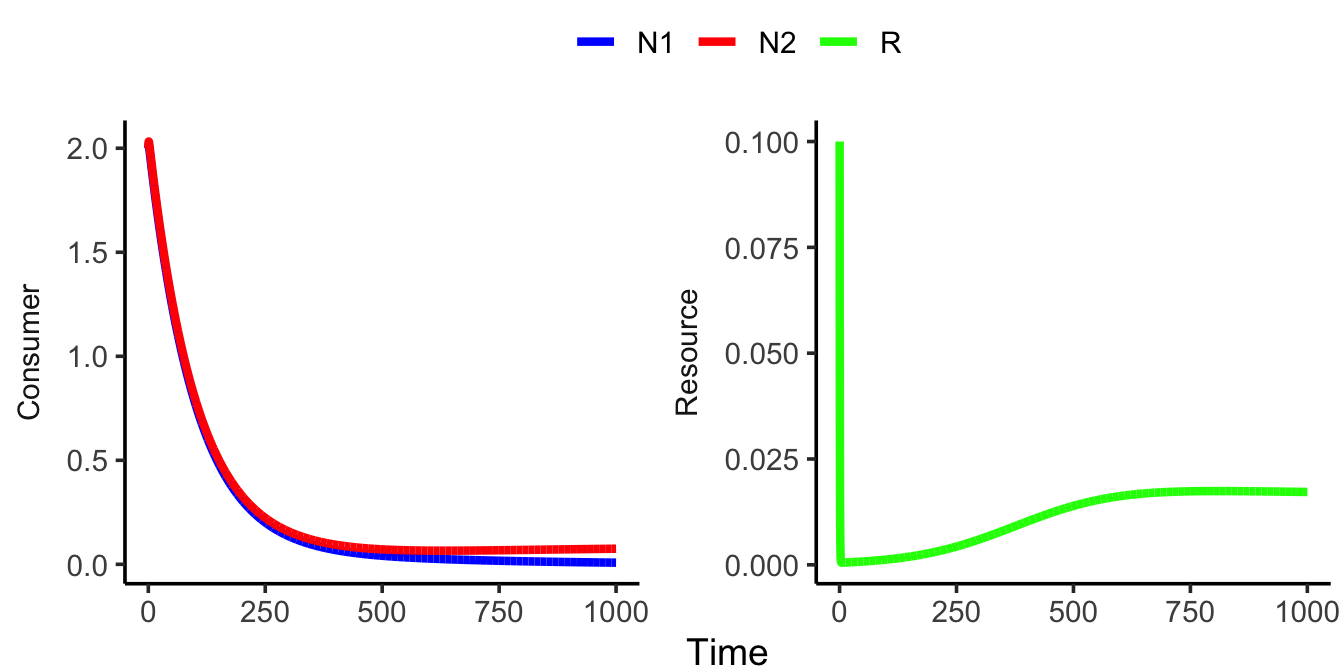
\includegraphics[width=0.9\linewidth]{bookdown-demo_files/figure-latex/unnamed-chunk-42-1} \end{center}

We can see that \(N_1\) goes extinct, as predicted by the R* rule; the remaining consumer \(N_2\) and the resource \(R\) exhibit stable coexistence.

\textbf{Part 2 - Tilman's resource ratio hypothesis}

Now we will extend the model in Part 1. into two consumers and two resources:
\begin{align*}
\frac {dN_{1}}{dt} &= e_{1}a_{1a}R_{a}N_{1}+e_{1}a_{1b}R_{b}N_{1}-dN_{1}\\
\frac {dN_{2}}{dt} &= e_{2}a_{2a}R_{a}N_{2}+e_{2}a_{2b}R_{b}N_{2}-dN_{2}\\
\frac {dR_{a}}{dt} &= d(S_{a}-R_{a})-a_{1a}R_{a}N_{1}-a_{2a}R_{a}N_{2}\\
\frac {dR_{b}}{dt} &= d(S_{b}-R_{b})-a_{1b}R_{b}N_{1}-a_{2b}R_{b}N_{2}\\
\end{align*}

Here, the two consumers \(N_1\) and \(N_2\) compete for two substitutable resources \(R_1\) and \(R_2\). Under certain conditions, the two consumers are able to coexist:

\begin{Shaded}
\begin{Highlighting}[]
\CommentTok{### Model specification}
\NormalTok{CR_model_2C_2R <-}\StringTok{ }\ControlFlowTok{function}\NormalTok{(time, state, parms)\{}
  \KeywordTok{with}\NormalTok{(}\KeywordTok{as.list}\NormalTok{(}\KeywordTok{c}\NormalTok{(state, parms)), \{}
\NormalTok{    dN1_dt =}\StringTok{ }\NormalTok{e1}\OperatorTok{*}\NormalTok{a1a}\OperatorTok{*}\NormalTok{Ra}\OperatorTok{*}\NormalTok{N1 }\OperatorTok{+}\StringTok{ }\NormalTok{e1}\OperatorTok{*}\NormalTok{a1b}\OperatorTok{*}\NormalTok{Rb}\OperatorTok{*}\NormalTok{N1 }\OperatorTok{-}\StringTok{ }\NormalTok{d}\OperatorTok{*}\NormalTok{N1}
\NormalTok{    dN2_dt =}\StringTok{ }\NormalTok{e2}\OperatorTok{*}\NormalTok{a2a}\OperatorTok{*}\NormalTok{Ra}\OperatorTok{*}\NormalTok{N2 }\OperatorTok{+}\StringTok{ }\NormalTok{e2}\OperatorTok{*}\NormalTok{a2b}\OperatorTok{*}\NormalTok{Rb}\OperatorTok{*}\NormalTok{N2 }\OperatorTok{-}\StringTok{ }\NormalTok{d}\OperatorTok{*}\NormalTok{N2}
\NormalTok{    dRa_dt =}\StringTok{ }\NormalTok{d}\OperatorTok{*}\NormalTok{(Sa}\OperatorTok{-}\NormalTok{Ra) }\OperatorTok{-}\StringTok{ }\NormalTok{(a1a}\OperatorTok{*}\NormalTok{N1}\OperatorTok{*}\NormalTok{Ra) }\OperatorTok{-}\StringTok{ }\NormalTok{(a2a}\OperatorTok{*}\NormalTok{N2}\OperatorTok{*}\NormalTok{Ra) }
\NormalTok{    dRb_dt =}\StringTok{ }\NormalTok{d}\OperatorTok{*}\NormalTok{(Sb}\OperatorTok{-}\NormalTok{Rb) }\OperatorTok{-}\StringTok{ }\NormalTok{(a1b}\OperatorTok{*}\NormalTok{N1}\OperatorTok{*}\NormalTok{Rb) }\OperatorTok{-}\StringTok{ }\NormalTok{(a2b}\OperatorTok{*}\NormalTok{N2}\OperatorTok{*}\NormalTok{Rb)}
    \KeywordTok{return}\NormalTok{(}\KeywordTok{list}\NormalTok{(}\KeywordTok{c}\NormalTok{(dN1_dt, dN2_dt, dRa_dt, dRb_dt)))}
\NormalTok{  \})}
\NormalTok{\}}

\CommentTok{### Model parameters}
\NormalTok{times <-}\StringTok{ }\KeywordTok{seq}\NormalTok{(}\FloatTok{0.1}\NormalTok{, }\DecValTok{2000}\NormalTok{, }\DataTypeTok{by =} \FloatTok{0.01}\NormalTok{)}
\NormalTok{state <-}\StringTok{ }\KeywordTok{c}\NormalTok{(}\DataTypeTok{N1 =} \FloatTok{0.05}\NormalTok{, }\DataTypeTok{N2 =} \FloatTok{0.05}\NormalTok{, }\DataTypeTok{Ra =} \FloatTok{0.3}\NormalTok{, }\DataTypeTok{Rb =} \FloatTok{0.3}\NormalTok{)}
\NormalTok{parms <-}\StringTok{ }\KeywordTok{c}\NormalTok{(}\DataTypeTok{a1a =} \FloatTok{0.4}\NormalTok{, }\DataTypeTok{a1b =} \FloatTok{0.8}\NormalTok{, }\DataTypeTok{a2a =} \FloatTok{0.6}\NormalTok{, }\DataTypeTok{a2b =} \FloatTok{0.5}\NormalTok{, }\DataTypeTok{e1 =} \DecValTok{1}\NormalTok{, }\DataTypeTok{e2 =} \DecValTok{1}\NormalTok{, }\DataTypeTok{d =} \FloatTok{0.1}\NormalTok{, }\DataTypeTok{Sa =} \FloatTok{0.3}\NormalTok{, }\DataTypeTok{Sb =} \FloatTok{0.3}\NormalTok{)  }

\CommentTok{### Model application}
\NormalTok{pop_size <-}\StringTok{ }\KeywordTok{ode}\NormalTok{(}\DataTypeTok{func =}\NormalTok{ CR_model_2C_2R, }\DataTypeTok{times =}\NormalTok{ times, }\DataTypeTok{y =}\NormalTok{ state, }\DataTypeTok{parms =}\NormalTok{ parms)}


\CommentTok{### Visualize the population dynamics}
\NormalTok{pop_size }\OperatorTok
\StringTok{  }\KeywordTok{as.data.frame}\NormalTok{() }\OperatorTok
\StringTok{  }\KeywordTok{gather}\NormalTok{(}\DataTypeTok{key =} \StringTok{"Species"}\NormalTok{, }\DataTypeTok{value =} \StringTok{"N"}\NormalTok{, N1}\OperatorTok{:}\NormalTok{Rb) }\OperatorTok
\StringTok{  }\KeywordTok{mutate}\NormalTok{(}\DataTypeTok{trophic =} \KeywordTok{case_when}\NormalTok{(Species }\OperatorTok\StringTok{ }\KeywordTok{c}\NormalTok{(}\StringTok{"N1"}\NormalTok{, }\StringTok{"N2"}\NormalTok{) }\OperatorTok{~}\StringTok{ "Consumer"}\NormalTok{,}
                             \OtherTok{TRUE} \OperatorTok{~}\StringTok{ "Resource"}\NormalTok{)) }\OperatorTok
\StringTok{  }\KeywordTok{ggplot}\NormalTok{(}\KeywordTok{aes}\NormalTok{(}\DataTypeTok{x =}\NormalTok{ time, }\DataTypeTok{y =}\NormalTok{ N, }\DataTypeTok{color =}\NormalTok{ Species)) }\OperatorTok{+}\StringTok{ }
\StringTok{  }\KeywordTok{geom_line}\NormalTok{(}\DataTypeTok{size =} \FloatTok{1.5}\NormalTok{) }\OperatorTok{+}
\StringTok{  }\KeywordTok{facet_wrap}\NormalTok{(}\OperatorTok{~}\StringTok{ }\NormalTok{trophic, }
             \DataTypeTok{ncol =} \DecValTok{2}\NormalTok{, }
             \DataTypeTok{scales =} \StringTok{"free_y"}\NormalTok{,}
             \DataTypeTok{strip.position =} \StringTok{"left"}\NormalTok{) }\OperatorTok{+}
\StringTok{  }\KeywordTok{theme_classic}\NormalTok{(}\DataTypeTok{base_size =} \DecValTok{14}\NormalTok{) }\OperatorTok{+}
\StringTok{  }\KeywordTok{theme}\NormalTok{(}\DataTypeTok{strip.background =} \KeywordTok{element_blank}\NormalTok{(),}
        \DataTypeTok{strip.placement =} \StringTok{"outside"}\NormalTok{,}
        \DataTypeTok{legend.position =} \StringTok{"top"}\NormalTok{,}
        \DataTypeTok{legend.title =} \KeywordTok{element_blank}\NormalTok{(),}
        \DataTypeTok{plot.margin =} \KeywordTok{margin}\NormalTok{(}\DataTypeTok{r =} \DecValTok{8}\NormalTok{)) }\OperatorTok{+}\StringTok{ }
\StringTok{  }\KeywordTok{labs}\NormalTok{(}\DataTypeTok{x =} \StringTok{"Time"}\NormalTok{, }\DataTypeTok{y =} \OtherTok{NULL}\NormalTok{) }\OperatorTok{+}
\StringTok{  }\KeywordTok{scale_x_continuous}\NormalTok{(}\DataTypeTok{limits =} \KeywordTok{c}\NormalTok{(}\DecValTok{0}\NormalTok{, }\DecValTok{2050}\NormalTok{), }\DataTypeTok{expand =} \KeywordTok{c}\NormalTok{(}\DecValTok{0}\NormalTok{, }\DecValTok{0}\NormalTok{)) }\OperatorTok{+}
\StringTok{  }\KeywordTok{scale_y_continuous}\NormalTok{(}\DataTypeTok{limits =} \KeywordTok{c}\NormalTok{(}\DecValTok{0}\NormalTok{, }\OtherTok{NA}\NormalTok{), }\DataTypeTok{expand =} \KeywordTok{c}\NormalTok{(}\DecValTok{0}\NormalTok{, }\DecValTok{0}\NormalTok{)) }\OperatorTok{+}
\StringTok{  }\KeywordTok{scale_color_manual}\NormalTok{(}\DataTypeTok{name =} \OtherTok{NULL}\NormalTok{, }\DataTypeTok{values =} \KeywordTok{c}\NormalTok{(}\StringTok{"blue"}\NormalTok{, }\StringTok{"red"}\NormalTok{, }\StringTok{"green"}\NormalTok{, }\StringTok{"purple"}\NormalTok{))}
\end{Highlighting}
\end{Shaded}

\begin{center}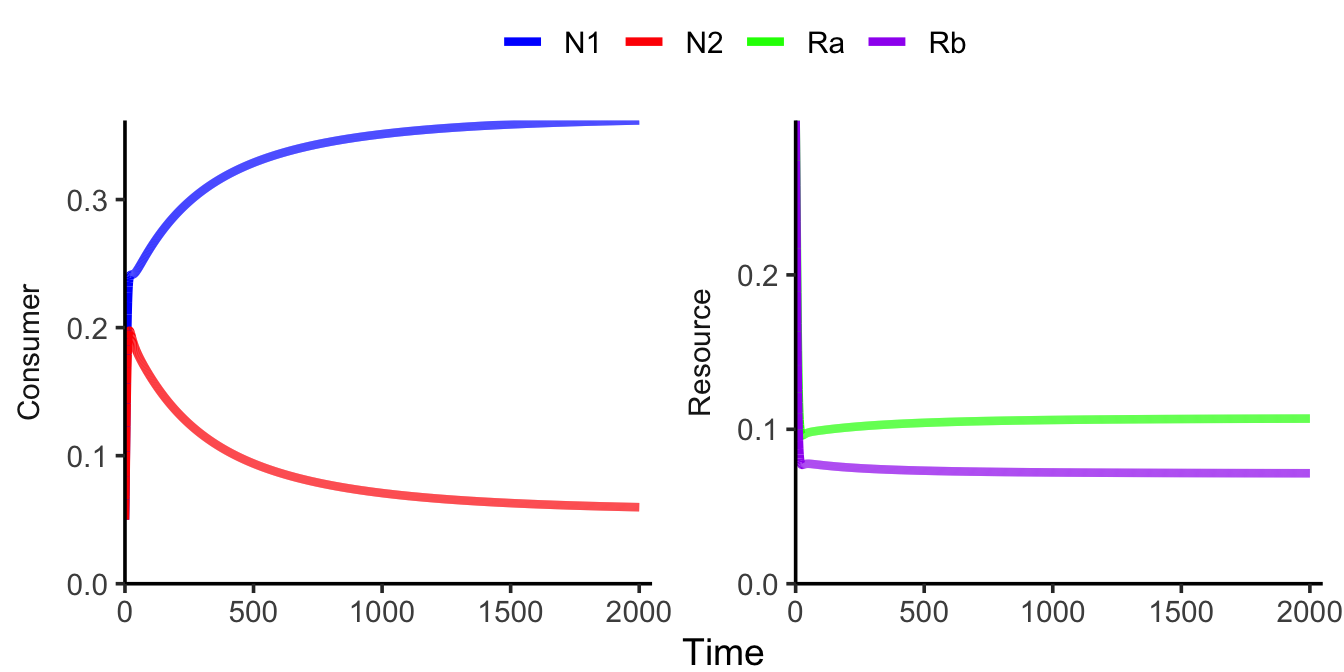
\includegraphics[width=0.9\linewidth]{bookdown-demo_files/figure-latex/unnamed-chunk-43-1} \end{center}

The phase diagram also illustrates stable coexistence of the two consumers:

\begin{Shaded}
\begin{Highlighting}[]
\CommentTok{### Parameters}
\NormalTok{a1a <-}\StringTok{ }\FloatTok{0.4}
\NormalTok{a1b <-}\StringTok{ }\FloatTok{0.8}
\NormalTok{a2a <-}\StringTok{ }\FloatTok{0.6}
\NormalTok{a2b <-}\StringTok{ }\FloatTok{0.5}
\NormalTok{e1 <-}\StringTok{ }\DecValTok{1}
\NormalTok{e2 <-}\StringTok{ }\DecValTok{1}
\NormalTok{d <-}\StringTok{ }\FloatTok{0.1}

\CommentTok{### Slopes and intercepts of the ZNGI's}
\NormalTok{ZNGI_slope_N1 <-}\StringTok{ }\OperatorTok{-}\NormalTok{a1a}\OperatorTok{/}\NormalTok{a1b}
\NormalTok{ZNGI_intercept_N1 <-}\StringTok{ }\NormalTok{d}\OperatorTok{/}\NormalTok{(e1}\OperatorTok{*}\NormalTok{a1b)  }
\NormalTok{ZNGI_slope_N2 <-}\StringTok{ }\OperatorTok{-}\NormalTok{a2a}\OperatorTok{/}\NormalTok{a2b}
\NormalTok{ZNGI_intercept_N2 <-}\StringTok{ }\NormalTok{d}\OperatorTok{/}\NormalTok{(e2}\OperatorTok{*}\NormalTok{a2b)}

\CommentTok{### Consumption vectors}
\NormalTok{eqilibrium_Ra <-}\StringTok{ }\NormalTok{(d}\OperatorTok{/}\NormalTok{e1)}\OperatorTok{*}\NormalTok{((a1b}\OperatorTok{-}\NormalTok{a2b)}\OperatorTok{/}\NormalTok{(a2a}\OperatorTok{*}\NormalTok{a1b}\OperatorTok{-}\NormalTok{a2b}\OperatorTok{*}\NormalTok{a1a))}
\NormalTok{eqilibrium_Rb <-}\StringTok{ }\NormalTok{(d}\OperatorTok{/}\NormalTok{e2)}\OperatorTok{*}\NormalTok{((a1a}\OperatorTok{-}\NormalTok{a2a)}\OperatorTok{/}\NormalTok{(a2b}\OperatorTok{*}\NormalTok{a1a}\OperatorTok{-}\NormalTok{a2a}\OperatorTok{*}\NormalTok{a1b))}

\NormalTok{convec_df <-}\StringTok{ }\KeywordTok{data.frame}\NormalTok{(}\DataTypeTok{x =} \KeywordTok{c}\NormalTok{(eqilibrium_Ra }\OperatorTok{+}\StringTok{ }\DecValTok{6}\OperatorTok{*}\NormalTok{a1a}\OperatorTok{*}\NormalTok{eqilibrium_Ra, }
\NormalTok{                              eqilibrium_Ra }\OperatorTok{+}\StringTok{ }\DecValTok{6}\OperatorTok{*}\NormalTok{a2a}\OperatorTok{*}\NormalTok{eqilibrium_Ra),}
                        \DataTypeTok{y =} \KeywordTok{c}\NormalTok{(eqilibrium_Rb }\OperatorTok{+}\StringTok{ }\DecValTok{6}\OperatorTok{*}\NormalTok{a1b}\OperatorTok{*}\NormalTok{eqilibrium_Rb, }
\NormalTok{                              eqilibrium_Rb }\OperatorTok{+}\StringTok{ }\DecValTok{6}\OperatorTok{*}\NormalTok{a2b}\OperatorTok{*}\NormalTok{eqilibrium_Rb),}
                        \DataTypeTok{xend =} \KeywordTok{c}\NormalTok{(eqilibrium_Ra }\OperatorTok{-}\StringTok{ }\NormalTok{a1a}\OperatorTok{*}\NormalTok{eqilibrium_Ra, }
\NormalTok{                              eqilibrium_Ra }\OperatorTok{-}\StringTok{ }\NormalTok{a2a}\OperatorTok{*}\NormalTok{eqilibrium_Ra),}
                        \DataTypeTok{yend =} \KeywordTok{c}\NormalTok{(eqilibrium_Rb }\OperatorTok{-}\StringTok{ }\NormalTok{a1b}\OperatorTok{*}\NormalTok{eqilibrium_Rb, }
\NormalTok{                              eqilibrium_Rb }\OperatorTok{-}\StringTok{ }\NormalTok{a2b}\OperatorTok{*}\NormalTok{eqilibrium_Rb),}
                        \DataTypeTok{species =} \KeywordTok{c}\NormalTok{(}\StringTok{"N1"}\NormalTok{, }\StringTok{"N2"}\NormalTok{))}

\CommentTok{### Phase diagram}
\KeywordTok{ggplot}\NormalTok{() }\OperatorTok{+}\StringTok{ }
\StringTok{  }\KeywordTok{geom_abline}\NormalTok{(}\DataTypeTok{slope =}\NormalTok{ ZNGI_slope_N1, }\DataTypeTok{intercept =}\NormalTok{ ZNGI_intercept_N1, }\DataTypeTok{color =} \StringTok{"#377EB8"}\NormalTok{, }\DataTypeTok{size =} \FloatTok{1.2}\NormalTok{) }\OperatorTok{+}\StringTok{ }
\StringTok{  }\KeywordTok{geom_abline}\NormalTok{(}\DataTypeTok{slope =}\NormalTok{ ZNGI_slope_N2, }\DataTypeTok{intercept =}\NormalTok{ ZNGI_intercept_N2, }\DataTypeTok{color =} \StringTok{"#E41A1C"}\NormalTok{, }\DataTypeTok{size =} \FloatTok{1.2}\NormalTok{) }\OperatorTok{+}\StringTok{ }
\StringTok{  }\KeywordTok{geom_segment}\NormalTok{(}\DataTypeTok{data =}\NormalTok{ convec_df, }\KeywordTok{aes}\NormalTok{(}\DataTypeTok{x =}\NormalTok{ x, }\DataTypeTok{y =}\NormalTok{ y, }\DataTypeTok{xend =}\NormalTok{ xend, }\DataTypeTok{yend =}\NormalTok{ yend, }\DataTypeTok{color =}\NormalTok{ species), }\DataTypeTok{linetype =} \StringTok{"blank"}\NormalTok{) }\OperatorTok{+}\StringTok{ }
\StringTok{  }\KeywordTok{geom_segment}\NormalTok{(}\DataTypeTok{data =}\NormalTok{ convec_df, }\KeywordTok{aes}\NormalTok{(}\DataTypeTok{x =}\NormalTok{ x, }\DataTypeTok{y =}\NormalTok{ y, }\DataTypeTok{xend =}\NormalTok{ xend, }\DataTypeTok{yend =}\NormalTok{ yend, }\DataTypeTok{color =}\NormalTok{ species), }\DataTypeTok{size =} \FloatTok{0.5}\NormalTok{, }\DataTypeTok{linetype =} \StringTok{"dashed"}\NormalTok{, }\DataTypeTok{arrow =} \KeywordTok{arrow}\NormalTok{(}\DataTypeTok{type =} \StringTok{"closed"}\NormalTok{, }\DataTypeTok{length =} \KeywordTok{unit}\NormalTok{(}\FloatTok{0.1}\NormalTok{, }\StringTok{"inches"}\NormalTok{)), }\DataTypeTok{show.legend =}\NormalTok{ F) }\OperatorTok{+}
\StringTok{  }\KeywordTok{geom_path}\NormalTok{(}\DataTypeTok{data =} \KeywordTok{as.data.frame}\NormalTok{(pop_size), }\KeywordTok{aes}\NormalTok{(}\DataTypeTok{x =}\NormalTok{ Ra, }\DataTypeTok{y =}\NormalTok{ Rb), }\DataTypeTok{size =} \FloatTok{1.2}\NormalTok{) }\OperatorTok{+}
\StringTok{  }\KeywordTok{geom_point}\NormalTok{(}\DataTypeTok{data =} \KeywordTok{as.data.frame}\NormalTok{(pop_size), }\KeywordTok{aes}\NormalTok{(}\DataTypeTok{x =} \KeywordTok{last}\NormalTok{(Ra), }\DataTypeTok{y =} \KeywordTok{last}\NormalTok{(Rb)), }\DataTypeTok{size =} \FloatTok{2.5}\NormalTok{) }\OperatorTok{+}
\StringTok{  }\KeywordTok{theme_classic}\NormalTok{(}\DataTypeTok{base_size =} \DecValTok{14}\NormalTok{) }\OperatorTok{+}
\StringTok{  }\KeywordTok{labs}\NormalTok{(}\DataTypeTok{x =} \KeywordTok{expression}\NormalTok{(}\KeywordTok{italic}\NormalTok{(R[a])), }\DataTypeTok{y =} \KeywordTok{expression}\NormalTok{(}\KeywordTok{italic}\NormalTok{(R[b]))) }\OperatorTok{+}
\StringTok{  }\KeywordTok{scale_x_continuous}\NormalTok{(}\DataTypeTok{limits =} \KeywordTok{c}\NormalTok{(}\DecValTok{0}\NormalTok{, }\FloatTok{0.5}\NormalTok{), }\DataTypeTok{expand =} \KeywordTok{c}\NormalTok{(}\DecValTok{0}\NormalTok{, }\DecValTok{0}\NormalTok{)) }\OperatorTok{+}
\StringTok{  }\KeywordTok{scale_y_continuous}\NormalTok{(}\DataTypeTok{limits =} \KeywordTok{c}\NormalTok{(}\DecValTok{0}\NormalTok{, }\FloatTok{0.5}\NormalTok{), }\DataTypeTok{expand =} \KeywordTok{c}\NormalTok{(}\DecValTok{0}\NormalTok{, }\DecValTok{0}\NormalTok{)) }\OperatorTok{+}
\StringTok{  }\KeywordTok{scale_color_brewer}\NormalTok{(}\DataTypeTok{name =} \OtherTok{NULL}\NormalTok{, }\DataTypeTok{palette =} \StringTok{"Set1"}\NormalTok{, }\DataTypeTok{direction =} \DecValTok{-1}\NormalTok{,}
                     \DataTypeTok{guide =} \KeywordTok{guide_legend}\NormalTok{(}\DataTypeTok{override.aes =} \KeywordTok{list}\NormalTok{(}
                       \DataTypeTok{linetype =} \StringTok{"solid"}\NormalTok{, }\DataTypeTok{size =} \FloatTok{1.2}\NormalTok{))) }\OperatorTok{+}
\StringTok{  }\KeywordTok{coord_fixed}\NormalTok{(}\DataTypeTok{ratio =} \DecValTok{1}\NormalTok{)}
\end{Highlighting}
\end{Shaded}

\begin{center}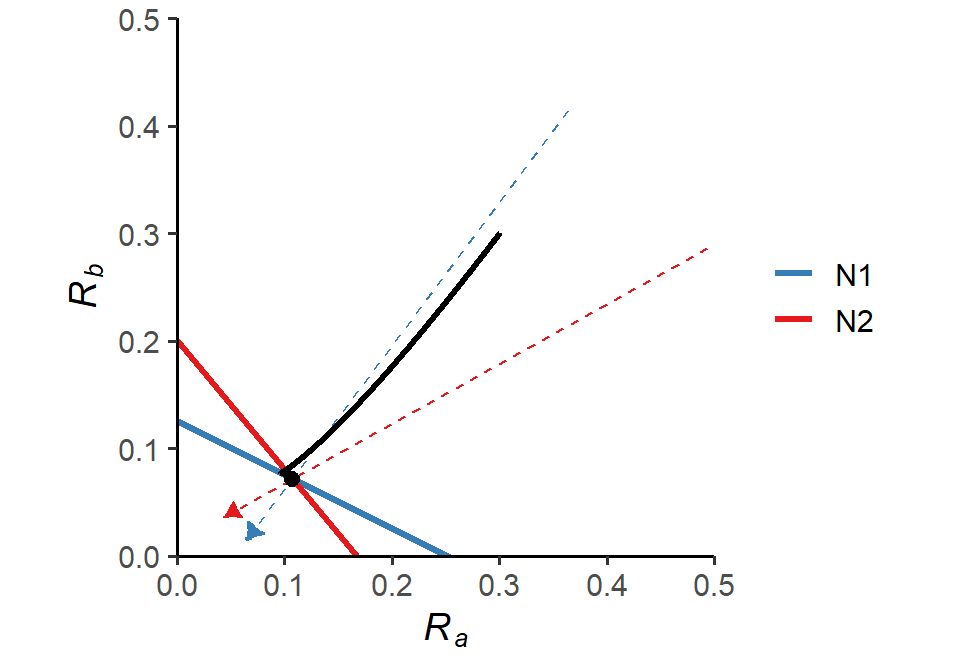
\includegraphics[width=0.7\linewidth]{bookdown-demo_files/figure-latex/unnamed-chunk-44-1} \end{center}

In this particular case, if the initial resource levels \(R_{a(0)}\) and \(R_{b(0)}\) fall within the upper area bounded by the two consumption vectors, then the two species will coexist.

\textbf{Part 3 - Relative nonlinearity}

We have seen in Part 1. that two species cannot coexist on one resource if the consumers consume it in a linear fashion. What if the consumers consume the resource in a non-linear fashion? Could that generate stable coexistence?

In this part of the lab section, we will introduce non-linear (type II) functional response into the consumer-resource model in Part 1. for one of the consumers. We also change the resource equation to logistic growth and allow the two consumers to have different conversion efficiencies and mortality rates:
\begin{align*}
\frac {dN_{1}}{dt} &= e_{1}a_{1}RN_{1}-d_{1}N_{1}\\
\frac {dN_{2}}{dt} &= e_{2}\frac{a_{2}R}{k_{2}+R}N_{2}-d_{2}N_{2}\\
\frac {dR}{dt} &= rR(1-\frac{R}{K})-a_{1}RN_{1}-\frac{a_{2}R}{k_{2}+R}N_{2}\\
\end{align*}

\begin{Shaded}
\begin{Highlighting}[]
\CommentTok{### Model specification}
\NormalTok{CR_model_nonlinear <-}\StringTok{ }\ControlFlowTok{function}\NormalTok{(times, state, parms)\{}
  \KeywordTok{with}\NormalTok{(}\KeywordTok{as.list}\NormalTok{(}\KeywordTok{c}\NormalTok{(state, parms)), \{}
\NormalTok{         dN1_dt =}\StringTok{ }\NormalTok{e1}\OperatorTok{*}\NormalTok{a1}\OperatorTok{*}\NormalTok{R}\OperatorTok{*}\NormalTok{N1 }\OperatorTok{-}\StringTok{ }\NormalTok{d1}\OperatorTok{*}\NormalTok{N1}
\NormalTok{         dN2_dt =}\StringTok{ }\NormalTok{e2}\OperatorTok{*}\NormalTok{(a2}\OperatorTok{*}\NormalTok{R}\OperatorTok{/}\NormalTok{(k2}\OperatorTok{+}\NormalTok{R))}\OperatorTok{*}\NormalTok{N2 }\OperatorTok{-}\StringTok{ }\NormalTok{d2}\OperatorTok{*}\NormalTok{N2}
\NormalTok{         dR_dt =}\StringTok{  }\NormalTok{r}\OperatorTok{*}\NormalTok{R}\OperatorTok{*}\NormalTok{(}\DecValTok{1}\OperatorTok{-}\NormalTok{(R}\OperatorTok{/}\NormalTok{K)) }\OperatorTok{-}\StringTok{ }\NormalTok{a1}\OperatorTok{*}\NormalTok{R}\OperatorTok{*}\NormalTok{N1 }\OperatorTok{-}\StringTok{ }\NormalTok{((a2}\OperatorTok{*}\NormalTok{R)}\OperatorTok{/}\NormalTok{(k2}\OperatorTok{+}\NormalTok{R))}\OperatorTok{*}\NormalTok{N2}
         \KeywordTok{return}\NormalTok{(}\KeywordTok{list}\NormalTok{(}\KeywordTok{c}\NormalTok{(dN1_dt, dN2_dt, dR_dt)))}
\NormalTok{       \})}
\NormalTok{\}}

\CommentTok{### Model parameters}
\NormalTok{times <-}\StringTok{ }\KeywordTok{seq}\NormalTok{(}\DecValTok{0}\NormalTok{, }\DecValTok{5000}\NormalTok{, }\DataTypeTok{by =} \FloatTok{0.1}\NormalTok{)  }
\NormalTok{state <-}\StringTok{ }\KeywordTok{c}\NormalTok{(}\DataTypeTok{N1 =} \FloatTok{0.3}\NormalTok{, }\DataTypeTok{N2 =} \DecValTok{19}\NormalTok{, }\DataTypeTok{R =} \DecValTok{106}\NormalTok{) }
\NormalTok{parms <-}\StringTok{ }\KeywordTok{c}\NormalTok{(}\DataTypeTok{a1 =} \FloatTok{0.003}\NormalTok{, }\DataTypeTok{a2 =} \FloatTok{0.5}\NormalTok{, }\DataTypeTok{k2 =} \DecValTok{50}\NormalTok{, }\DataTypeTok{e1 =} \FloatTok{0.33}\NormalTok{, }\DataTypeTok{e2 =} \FloatTok{0.3}\NormalTok{, }\DataTypeTok{d1 =} \FloatTok{0.11}\NormalTok{, }\DataTypeTok{d2 =} \FloatTok{0.1}\NormalTok{, }\DataTypeTok{r =} \FloatTok{0.1}\NormalTok{, }\DataTypeTok{K =} \DecValTok{300}\NormalTok{)}

\CommentTok{### Model application}
\NormalTok{pop_size <-}\StringTok{ }\KeywordTok{ode}\NormalTok{(}\DataTypeTok{func =}\NormalTok{ CR_model_nonlinear, }\DataTypeTok{times =}\NormalTok{ times, }\DataTypeTok{y =}\NormalTok{ state, }\DataTypeTok{parms =}\NormalTok{ parms)}

\CommentTok{### Visualize the population dynamics}
\NormalTok{pop_size }\OperatorTok
\StringTok{  }\KeywordTok{as.data.frame}\NormalTok{() }\OperatorTok
\StringTok{  }\KeywordTok{gather}\NormalTok{(}\DataTypeTok{key =} \StringTok{"Species"}\NormalTok{, }\DataTypeTok{value =} \StringTok{"N"}\NormalTok{, N1}\OperatorTok{:}\NormalTok{R) }\OperatorTok
\StringTok{  }\KeywordTok{mutate}\NormalTok{(}\DataTypeTok{trophic =} \KeywordTok{case_when}\NormalTok{(Species }\OperatorTok\StringTok{ }\KeywordTok{c}\NormalTok{(}\StringTok{"N1"}\NormalTok{, }\StringTok{"N2"}\NormalTok{) }\OperatorTok{~}\StringTok{ "Consumer"}\NormalTok{,}
                             \OtherTok{TRUE} \OperatorTok{~}\StringTok{ "Resource"}\NormalTok{)) }\OperatorTok
\StringTok{  }\KeywordTok{ggplot}\NormalTok{(}\KeywordTok{aes}\NormalTok{(}\DataTypeTok{x =}\NormalTok{ time, }\DataTypeTok{y =}\NormalTok{ N, }\DataTypeTok{color =}\NormalTok{ Species)) }\OperatorTok{+}\StringTok{ }
\StringTok{  }\KeywordTok{geom_line}\NormalTok{() }\OperatorTok{+}
\StringTok{  }\KeywordTok{facet_wrap}\NormalTok{(}\OperatorTok{~}\StringTok{ }\NormalTok{trophic, }
             \DataTypeTok{ncol =} \DecValTok{2}\NormalTok{, }
             \DataTypeTok{scales =} \StringTok{"free_y"}\NormalTok{,}
             \DataTypeTok{strip.position =} \StringTok{"left"}\NormalTok{) }\OperatorTok{+}
\StringTok{  }\KeywordTok{theme_classic}\NormalTok{(}\DataTypeTok{base_size =} \DecValTok{14}\NormalTok{) }\OperatorTok{+}
\StringTok{  }\KeywordTok{theme}\NormalTok{(}\DataTypeTok{strip.background =} \KeywordTok{element_blank}\NormalTok{(),}
        \DataTypeTok{strip.placement =} \StringTok{"outside"}\NormalTok{,}
        \DataTypeTok{legend.position =} \StringTok{"top"}\NormalTok{,}
        \DataTypeTok{legend.title =} \KeywordTok{element_blank}\NormalTok{(),}
        \DataTypeTok{plot.margin =} \KeywordTok{margin}\NormalTok{(}\DataTypeTok{r =} \DecValTok{5}\NormalTok{)) }\OperatorTok{+}\StringTok{ }
\StringTok{  }\KeywordTok{labs}\NormalTok{(}\DataTypeTok{x =} \StringTok{"Time"}\NormalTok{, }\DataTypeTok{y =} \OtherTok{NULL}\NormalTok{) }\OperatorTok{+}
\StringTok{  }\KeywordTok{scale_color_manual}\NormalTok{(}\DataTypeTok{name =} \OtherTok{NULL}\NormalTok{, }\DataTypeTok{values =} \KeywordTok{c}\NormalTok{(}\StringTok{"blue"}\NormalTok{, }\StringTok{"red"}\NormalTok{, }\StringTok{"green"}\NormalTok{))}
\end{Highlighting}
\end{Shaded}

\begin{center}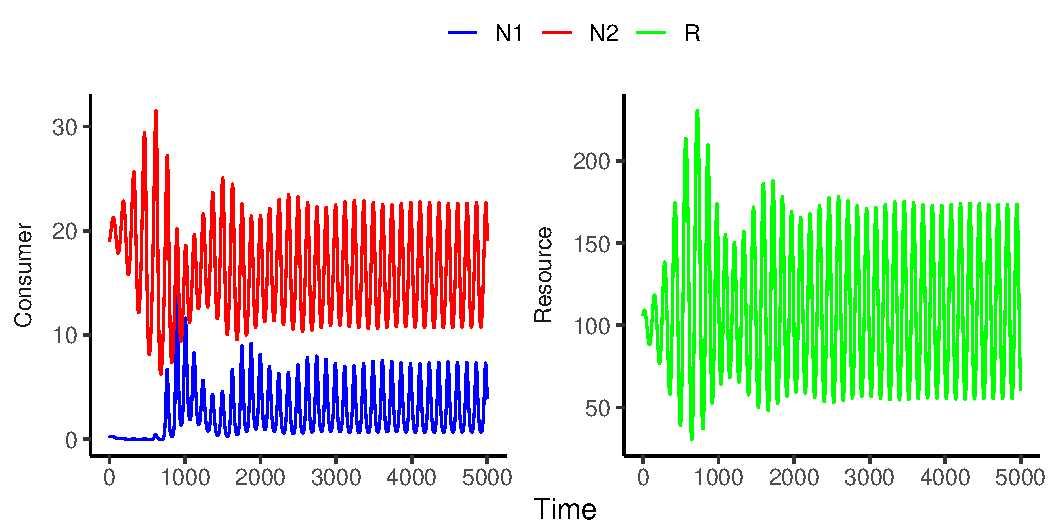
\includegraphics[width=0.9\linewidth]{bookdown-demo_files/figure-latex/unnamed-chunk-45-1} \end{center}

As shown in the figure, the two consumers coexist in a fluctuating manner. In fact, the fluctuating properties generated by the combination of logistically growing resources and different nonlinear functions are critical for the coexistence of \(n\) species on \(k<n\) resources in certain parameter spaces.

\hypertarget{week-15---research-applications-modern-coexistence-theory-and-plant-soil-feedback}{%
\chapter*{Week 15 - Research applications: modern coexistence theory and plant-soil feedback}\label{week-15---research-applications-modern-coexistence-theory-and-plant-soil-feedback}}
\addcontentsline{toc}{chapter}{Week 15 - Research applications: modern coexistence theory and plant-soil feedback}

\hypertarget{week-16---final-exam}{%
\chapter*{Week 16 - Final exam}\label{week-16---final-exam}}
\addcontentsline{toc}{chapter}{Week 16 - Final exam}

  \bibliography{book.bib,packages.bib}

\end{document}
